% !TEX TS-program = LuaLaTeX
\documentclass[11pt]{ltjsarticle}


%フォント(和文) japreset を使うことによって、一括に管理するようにしている。
\usepackage[hiragino-pron,jis2004,
deluxe%明朝体・ゴシック体各3ウェイトと,丸ゴシック体(mg)を利用可能にする
,bold%明朝体太字をゴシック体太字によって代替する.
]{luatexja-preset}
%\renewcommand{\kanjifamilydefault}{\gtdefault}% 既定をゴシック体に

\usepackage[height=8.8in,width=6.45in]{geometry}



%数式フォント
\usepackage{mathptmx}
\usepackage[scaled]{helvet}
\renewcommand{\ttdefault}{pcr}

\usepackage{mathtools} %extended amsmath
\usepackage{amssymb}
%\mathtoolsset{showonlyrefs=true,showmanualtags}%represent the number of equation when quote eqref
%\mathtoolsset{showonlyrefs,showmanualtags}
%\usepackage[warnings-off={mathtools-colon}]{unicode-math}


% not understanded
\countdef\cpart=1
\def\part#1{%
\newpage
\advance\cpart by 1
\section*{Part \the\cpart: #1}
\addcontentsline{toc}{section}{Part \the\cpart: #1}
%
}
\usepackage[nottoc]{tocbibind}

\usepackage{bm} %boldmath
\usepackage{mathdots}
\usepackage{ulem}


%????? これが効かないので一時的に外す。

\usepackage{graphicx} % include graphic
\usepackage{float}
\usepackage[svgnames]{xcolor}%(xcolor.pdf p38~39)

\usepackage{tensor}%for part 1 relativity

\usepackage{enumerate}
\usepackage{adjustbox}
\usepackage[
 unicode=true,
 colorlinks=true,
 bookmarks=true,
 bookmarksnumbered=true,
 pdftitle={notes},% タイトル
 pdfsubject={relativity},% サブタイトル
 pdfauthor={Shun Taniwaki},% 著者
 pdfkeywords={Weinberg-Cosmology}% キーワード
 citecolor=DarkGreen,
 linkcolor=FireBrick,
 %urlcolor=FireBrick,
 linktocpage=true,
]{hyperref}

%\usepackage{pxjahyper} ドライバ依存パッケージ
\usepackage[thref,amsmath,thmmarks]{ntheorem}

\theoremstyle{plain}
\theorembodyfont{\normalfont}
%\theoremsymbol{\text{\normalfont (Q.E.D.)}}
\theoremseparator{.}
\theoremstyle{break}

\usepackage{mdframed}
\newmdtheoremenv[ntheorem,backgroundcolor=black!10,linecolor=black!0]{principle}{原理}[section]
\newmdtheoremenv[ntheorem,backgroundcolor=black!10,linecolor=black!0]{assumption}{仮定}[section]
\newmdtheoremenv[ntheorem,backgroundcolor=black!10,linecolor=black!0]{definition}{定義}[section]
\newmdtheoremenv[ntheorem,backgroundcolor=black!10,linecolor=black!0]{formula}{公式}[section]
%\newmdtheoremenv[ntheorem,backgraoudcolor=black!0]{theorem}{定理}[subsection]
\newmdtheoremenv[ntheorem,backgroundcolor=black!10]{theorem}[definition]{事実}
\newmdtheoremenv[ntheorem,backgroundcolor=black!3,linecolor=black!0]{example}{(計算)例}[definition]
\newmdtheoremenv[ntheorem,backgroundcolor=black!0]{unclear}{Unclear points}[section]
%\newmdtheoremenv[mdframedoption]{envname}[numberedlike]{caption} [within]


\usepackage{tikz}
\usepackage[compat=1.1.0]{tikz-feynman} %前に配置すると、xcolorと喧嘩する。

\mathtoolsset{showonlyrefs,showmanualtags}

% def bold faces
\bmdefine{\bfa}{a}
\bmdefine{\bfb}{b}
\bmdefine{\bfc}{c}
\bmdefine{\bfd}{d}
\bmdefine{\bfe}{e}
\bmdefine{\bff}{f}
\bmdefine{\bfg}{g}
\bmdefine{\bfh}{h}
\bmdefine{\bfi}{i}
\bmdefine{\bfj}{j}
\bmdefine{\bfk}{k}
\bmdefine{\bfl}{l}
\bmdefine{\bfm}{m}
\bmdefine{\bfn}{n}
\bmdefine{\bfo}{o}
\bmdefine{\bfp}{p}
\bmdefine{\bfq}{q}
\bmdefine{\bfr}{r}
\bmdefine{\bfs}{s}
\bmdefine{\bft}{t}
\bmdefine{\bfu}{u}
\bmdefine{\bfv}{v}
\bmdefine{\bfw}{w}
\bmdefine{\bfx}{x}
\bmdefine{\bfy}{y}
\bmdefine{\bfz}{z}
\bmdefine{\bfA}{A}
\bmdefine{\bfB}{B}
\bmdefine{\bfC}{C}
\bmdefine{\bfD}{D}
\bmdefine{\bfE}{E}
\bmdefine{\bfF}{F}
\bmdefine{\bfG}{G}
\bmdefine{\bfH}{H}
\bmdefine{\bfI}{I}
\bmdefine{\bfJ}{J}
\bmdefine{\bfK}{K}
\bmdefine{\bfL}{L}
\bmdefine{\bfM}{M}
\bmdefine{\bfN}{N}
\bmdefine{\bfO}{O}
\bmdefine{\bfP}{P}
\bmdefine{\bfQ}{Q}
\bmdefine{\bfR}{R}
\bmdefine{\bfS}{S}
\bmdefine{\bfT}{T}
\bmdefine{\bfU}{U}
\bmdefine{\bfV}{V}
\bmdefine{\bfW}{W}
\bmdefine{\bfX}{X}
\bmdefine{\bfY}{Y}
\bmdefine{\bfZ}{Z}
\bmdefine{\bftheta}{\theta}
\bmdefine{\bfphi}{\varphi}
\bmdefine{\bfomega}{\omega}




%mathbf
\newcommand{\mbfa}{\mathbf{a}}
\newcommand{\mbfb}{\mathbf{b}}
\newcommand{\mbfc}{\mathbf{c}}
\newcommand{\mbfd}{\mathbf{d}}
\newcommand{\mbfe}{\mathbf{e}}
\newcommand{\mbff}{\mathbf{f}}
\newcommand{\mbfg}{\mathbf{g}}
\newcommand{\mbfh}{\mathbf{h}}
\newcommand{\mbfi}{\mathbf{i}}
\newcommand{\mbfj}{\mathbf{j}}
\newcommand{\mbfk}{\mathbf{k}}
\newcommand{\mbfl}{\mathbf{l}}
\newcommand{\mbfm}{\mathbf{m}}
\newcommand{\mbfn}{\mathbf{n}}
\newcommand{\mbfo}{\mathbf{o}}
\newcommand{\mbfp}{\mathbf{p}}
\newcommand{\mbfq}{\mathbf{q}}
\newcommand{\mbfr}{\mathbf{r}}
\newcommand{\mbfs}{\mathbf{s}}
\newcommand{\mbft}{\mathbf{t}}
\newcommand{\mbfu}{\mathbf{u}}
\newcommand{\mbfv}{\mathbf{v}}
\newcommand{\mbfw}{\mathbf{w}}
\newcommand{\mbfx}{\mathbf{x}}
\newcommand{\mbfy}{\mathbf{y}}
\newcommand{\mbfz}{\mathbf{z}}
\newcommand{\mbfA}{\mathbf{A}}
\newcommand{\mbfB}{\mathbf{B}}
\newcommand{\mbfC}{\mathbf{C}}
\newcommand{\mbfD}{\mathbf{D}}
\newcommand{\mbfE}{\mathbf{E}}
\newcommand{\mbfF}{\mathbf{F}}
\newcommand{\mbfG}{\mathbf{G}}
\newcommand{\mbfH}{\mathbf{H}}
\newcommand{\mbfI}{\mathbf{I}}
\newcommand{\mbfJ}{\mathbf{J}}
\newcommand{\mbfK}{\mathbf{K}}
\newcommand{\mbfL}{\mathbf{L}}
\newcommand{\mbfM}{\mathbf{M}}
\newcommand{\mbfN}{\mathbf{N}}
\newcommand{\mbfO}{\mathbf{O}}
\newcommand{\mbfP}{\mathbf{P}}
\newcommand{\mbfQ}{\mathbf{Q}}
\newcommand{\mbfR}{\mathbf{R}}
\newcommand{\mbfS}{\mathbf{S}}
\newcommand{\mbfT}{\mathbf{T}}
\newcommand{\mbfU}{\mathbf{U}}
\newcommand{\mbfV}{\mathbf{V}}
\newcommand{\mbfW}{\mathbf{W}}
\newcommand{\mbfX}{\mathbf{X}}
\newcommand{\mbfY}{\mathbf{Y}}
\newcommand{\mbfZ}{\mathbf{Z}}
%tilde
\newcommand{\tilg}{\tilde{g}}
\newcommand{\tilGamma}{\tilde{\Gamma}}
%****
\def\TODO#1{{\color{FireBrick} #1}}
%***
\newcommand{\Slash}[1]{{\ooalign{\hfil/\hfil\crcr$#1$}}}%スラッシュ引くよう

\def\ii{\mathrm{i}}
\def\Nequals#1{$\mathcal{N}{=}\,#1$}

%def tensors
\newcommand{\tensorR}[1]{\tensor{R}{ #1}}
\newcommand{\tensorGamma}[1]{\tensor{\Gamma}{ #1}}
\newcommand{\tensorG}[1]{\tensor{G}{ #1}}
\newcommand{\tensorg}[1]{\tensor{g}{ #1}}

%def math operators
\DeclareMathOperator{\arcsinh}{arcsinh}
\def\odi#1#2{\frac{d #1}{d #2}} %ordinary differential
\def\todi#1#2{\frac{d^{2} #1}{d #2^{2}}} %two ordinary differential
\newcommand{\pdi}[2]{\frac{\partial #1}{\partial #2}}%partial differential
\newcommand{\tpdi}[2]{\frac{\partial #1^{2}}{\partial #2^{2}}}%two partial differential
\def\vev#1{\Bigl(#1\Bigr)}% Vacume Expectation Value ?
\DeclareMathOperator{\sign}{sign}% sign
\def\diag{\mathop{\mathrm{diag}}\nolimits}% diagonalize
\def\tr{\mathop{\mathrm{tr}}\nolimits}% trace
\def\adj{\mathop{\mathrm{adj}}}% adjoint

%*********************************************************************

%def alert
\def\alert#1{\textbf{\textcolor{red}{\uwave{#1}}}}
%*********************************************************************

%\pagestyle{empty}
\begin{document}

\begin{flushright}
ゼミノート
\end{flushright}

\vskip 4cm

\begin{center}

{\Large \adjustbox{bgcolor=green}{Notes}}


\vskip 1cm
 Shunsuke Taniwaki
\vskip 1cm

\begin{tabular}{ll}
  & 基幹教育院粒子系理論物理学研究室\\
  & 九州大学 819-0395 福岡県福岡市西区元岡744 (センター3号館)
\end{tabular}

\vskip 1cm

\end{center}

\noindent
このノートは、私がWeinberg の Cosmology のレビューノート\footnote{\href{https://en.wikipedia.org/wiki/Donald_Knuth}{クヌース先生}に感謝申し上げる。
}である。
パート(章)で内容が独立に区切られるように設定してある。
なお、現時点(\today)において、このノートは\Nequals{1}部で構成されている:

\smallskip

\noindent\textbf{Part 1:}
本章は、宇宙の膨張についてである。
まずはじめに、宇宙は一様(homogeneous)かつ等方(isotorpic)であるという仮定のもとで、Robertson-Walker 計量を導出し、調べる(\ref{sec:Space-geometry}節)。歴史的には、Fredmann がアインシュタイン方程式の解として、最初に調べ、RobertsonとWalker が等方性および一様性の仮定のみから導いた。
次に、これらの仮定の観測的意義をを議論する(\ref{sec:The-cosmological-redshift}-\ref{sec:Luminosity-distances-and-angular-diameter-distances}節)。
そして、Robertson-Walker 計量をアインシュタイン方程式に適用する(\ref{sec:Dynamics-of-expansion}節)。
最後に、それらの結果、帰結について調べる(\ref{sec:Distances-at-large-redshift}-\ref{sec:Horizons}節)。
まああといろいろあるが、まだわからん。


%\end{titlepage}



\setcounter{tocdepth}{3}
\tableofcontents

\newpage
%
%************************************************************************************************************
%Part 1
%***********************************************************************************************************

\setcounter{section}{-1}
\section{Premalies}
Weinberg 特有のノーテーションや記号の定義について述べる。

\setcounter{section}{0}
\part{THE EXPANSINON OF THE UNIVERSE}\label{part:THE EXPANSINON-OF-THE-UNIVERSE}

\section{Space geometry}\label{sec:Space-geometry}
There are only three spaces that is  homogeneous and isotropic:\\
Spherical space :
\begin{align}
ds^2 = d\mbfx^2.
\end{align}
Hypersherical space :
\begin{align}
ds^2 = d\mbfx^2 -dz^2,\quad z^2 +\mbfx^2 = a^2
\end{align}
Euclidean space :
\begin{align}
ds^2 = d\mbfx^2 -dz^2,\quad z^2 - \mbff^2 =a^2\\
\end{align}%

From the asuumption that the universe is isotorpic and homogeneous,
we can define the spacetime line element
(with the Robertson – Walker scale factor):
\begin{align}
  d\tau^2
  :=& - \tensorg{_{\mu\nu}}dx^\mu dx^\nu \\
  =& dt^2 - ds^2 \\
  =& dt^2 - a^2(t) [d\mbfx^2 + K\frac{(\mbfx\cdot d\mbfx)^2}{1-K\mbfx^2}]
\end{align}
Then, we can calculate the Robertson–Walker metric:
\begin{align}
  g_{ij} = a^2(t)(\delta_{ij} + K\frac{x_i x_j}{1-K\mbfx^2}),\quad g_{i0}=0,\quad g_{00} = -1
\end{align}
Instead of the quasi-Cartesian coordinates $x_i$,we can use spherical polar coordinates, for which:
\begin{align}
  d\mbfx^2
  &= dr^2 + r^2 d\Omega\\
  &:= dr^2 + r^2(d\theta^2 + \sin^2\theta d\phi^2)
\end{align}
so,
\begin{align}
  d\tau^2 = dt^2 - a^2(t)[\frac{dr^2}{1-Kr^2} + r^2 d\Omega]
\end{align}
In which case the metric becomes diagonal:
\begin{align}
  g_{rr} = \frac{a^2(t)}{1-Kr^2},\quad g_{\theta\theta}= a^2(t)r^2,\quad g_{\phi\phi}= a^2(t)r^2 \sin^2\theta, \quad g_{00} = -1
\end{align}
The equation of motion of freely falling particles is given as:
\begin{align}
  \frac{d^2 x^\mu}{du^2} + \tensorGamma{^\mu_{\nu\kappa}} \frac{dx^\mu}{du}\frac{dx^\kappa}{du} = 0
  \label{eq:geodesic-equation}
\end{align}
where, $u$ is  a suitable variable parameterizing positions along the spacetime curve, proportional to $\tau$ for massive particles. \\%some scalar quantity that parameterizes position along the particle's trajectory
Remark that the first derivative of the coordinate $x^\mu :\frac{dx^\mu}{du}$ is a vector:
\begin{align}
  \frac{dx^{\prime \rho}}{du} = \frac{\partial x^{\prime \rho}}{\partial x^\mu}\frac{dx^\mu}{du}
\end{align}
but the second derivative $\todi{x^\mu}{u}$  is not a vector, because:
\begin{align}
  \todi{x^{\prime \rho}}{u}
  &= \frac{d}{du}(\pdi{x^{\prime \rho}}{x^\mu} \odi{x^\mu}{u})\\
  &= \pdi{x^{\prime \rho}}{x^\mu} \todi{x^\mu}{u} + \frac{\partial^2 x^{\prime \rho}}{\partial x^\mu \partial x^\mu} \frac{d x^\mu}{du}\frac{dx^\nu}{du}
\end{align}
We have defined the affine connection:$\tensorGamma{^{^nu}_{\mu \kappa}}$ as:
\begin{align}
  \tensorGamma{^{^nu}_{\mu \kappa}} = \frac{1}{2}g^{\mu \lambda}[ \frac{\partial g_{\lambda \mu}}{\partial x^{\kappa}} + \frac{\partial g_{\lambda \kappa}}{\partial x^\mu} - \frac{\partial g_{\mu \kappa}}{\partial x^\lambda}] \label{eq:christoffel-symbols}
\end{align}
A spacetime path $x^\mu = x^\mu(u)$ satisfying geodesic-equation(Eq.\eqref{eq:geodesic-equation}) is said to be a \textit{geodesic}, meaning that integral $\int d\tau$ is stationary under any infinitesimal variation of the path that leaves the endpoints fixed.

Note in particular that the derivatives $\partial_\mu g_{00},\,\, \partial_0 g_{0\mu}$ vanish.\footnote{%
Textbook says that $\partial_i g_{00}= \partial_0 g_{0i}$ vanish. }%
, because $g_{00}=-1, \text{and} \,\, g_{0i}=-1$ , so
\begin{align}
  \tensorGamma{^i_{00}}
  &= \frac{1}{2}g^{i\lambda}(\frac{g_{\lambda 0}}{\partial x^0}+\frac{g_{\lambda 0}}{\partial x^0} - \underbrace{\frac{g_{00}}{\partial x^\lambda}}_{0}) \\
  &=\tensorg{^{i \lambda}}\frac{g_{\lambda 0}}{\partial x^0} \\
  &= 0
\end{align}
A particle at rest in these coordinates will therefore stay at rest, so these are co-moving coordinates, which follow the motion of typical observers.
\begin{align}
  \frac{d^2 x^{i}}{du^{2}} + \tensorGamma{^i_{00}}\frac{dx^0}{du}\frac{dx^0}{du}
  + 2 \tensorGamma{^i_{0j}}\frac{dx^j}{du}\frac{dx^0}{du}
  + \tensorGamma{^i_{jk}}\frac{dx^j}{du}\frac{dx^\kappa}{du} &= 0\\
  \rightarrow \quad \frac{d^2 x^{i}}{du^{2}} +( \text{terms of } \frac{dx^i}{du}) &=0
\end{align}
 The proper time interval: $d\tau = \sqrt{-g_{\mu\nu}dx^\mu dx^\nu}$ for a co-moving clock ($d\mbfx=0$) is just dt, so $t$ is the time measured in ther est frame of co-moving clock.

The proper distance at time $t$ from the origin to a co-moving object at radial coordinate $r$:
\footnote{$r$ is radial coordinate.}
\begin{align}
  d(r,t)
  &= a(t) \int_0^r \frac{dr}{1-Kr^2}
    =a(t)\times
  		\begin{cases}
                  \arcsin r  & K=+1\\
                  \arcsinh r & K=-1\\
                  r              & K=0
               \end{cases}
\end{align}
In this coordinate system a co-moving object has $r$ time-independent, so the proper distance from us to a co-moving object increases (or decreases) with $a(t)$.
Since there is nothing special about our own position,\footnote{宇宙原理?一様であるということ。} the proper distance between any two co-moving observers anywhere in the universe must also be proportional to $a(t)$.
The rate of change of any such proper distance $d(t)$ is just:
\begin{align}
  \dot{d} = d\frac{\dot{a}}{a}
\end{align}

%We also need
The non-zero components of the affine connection are given by Eq.(\ref{eq:christoffel-symbols}) as:
\begin{align}
  \tensorGamma{^{0}_{ij}}
  &=\frac{1}{2}g^{0\lambda}[\frac{\partial g_{\lambda i}}{\partial x^j} + \frac{\partial g_{\lambda j}}{\partial x^i} -\frac{\partial g_{ij}}{\partial x^\lambda}] \\
  &=\frac{1}{2} g^{00}[\frac{\partial g_{0i}}{\partial x^j} + \frac{\partial g_{0i}}{\partial x^i} -\frac{\partial g_{ij}}{\partial x^0}]\quad(\because\,\,g^{0i}=0)\\
  &=\frac{1}{2} \frac{\partial g_{ij}}{\partial x^0}\\
  &=a \dot{a} \tilde{g}_{ij}
\end{align}
\begin{align}
  \tensorGamma{^{i}_{0j}}
  &=\frac{1}{2}g^{i \lambda}[\frac{\partial g_{\lambda 0}}{\partial x^j}+\frac{\partial g_{\lambda j}}{\partial x^0} -\frac{g_{0j}}{\partial x^\lambda}] \\
  &=\frac{1}{2}g^{i l}[\frac{\partial g_{l 0}}{\partial x^j}+\frac{\partial g_{l j}}{\partial x^0} -\frac{g_{0j}}{\partial x^l}]\quad(\lambda \to l)\\
  &=\frac{1}{2}g^{i l}\frac{\partial g_{lj}}{\partial x^0} \quad(\because\,\,g_{00}=-1,g_{i0}=0)\\
  &=\frac{1}{2} 2 a \dot{a}\frac{1}{a^2}g^{il}g_{lj}\\
  &=\frac{\dot{a}}{a} \tensor{\delta}{^i_j}
\end{align}%
Here $\tilde{g}_{ij}$ and $\tensor{\tilde{\Gamma}}{^{i}_{jl}}$ are the purely spatial metric and affine connection, and  $\tilde{g}^{ij}$ is the reciprocal of the $3\times3$ matrix $\tilde{g}_{ij}$
In quasi-Cartesian coordinates, $\tilde{g}_{ij}$ and $\tensor{\tilde{\Gamma}}{^{i}_{jl}}$:
\begin{align}
\tilde{g}_{ij} = \delta_{ij} + K \frac{x_i x_j}{1-K\mbfx^2}
\end{align}
\begin{align}
\tensor{\tilde{\Gamma}}{^{i}_{jl}} = K \tilde{g}_{ij} x^i \label{eq:1-1-20}
\end{align}%
To derive this relation \eqref{eq:1-1-20}, we need $\tilde{g}^{ik}$.\\
Definiton of $\tilde{g}^{ik}$:
\begin{align}
\tilde{g}^{ik}\tilde{g}_{kj} = \tensor{\delta}{^i_j}
\end{align}%
We assume that the form of $\tilde{g}^{ik}$ as follows: \footnote{Thanks to 原田恒司先生}
$\tilde{g}^{ik}= (A \tensor{\delta}{^{ik}} + Bx^i x^k)$
, then, using definition of reciprocal :
\begin{align}
\tilde{g}^{ik}\tilde{g}_{kj} &= \tensor{\delta}{^i_j} \\
(A \tensor{\delta}{^{ik}} + Bx_i x_k) (\delta_{kj} + K \frac{x_k x_j}{1- K \mbfx^2} ) & =  \tensor{\delta}{^i_j} \\
A \tensor{\delta}{^{ik}} \delta_{kj} + Bx_i x_k \delta_{kj} +A \tensor{\delta}{^{ik}}K \frac{x_k x_j}{1- K \mbfx^2} +Bx_i x_k K \frac{x_k x_j}{1- K \mbfx^2} & =  \tensor{\delta}{^i_j} \\
A \tensor{\delta}{^{i}_j} + Bx_i x_j  +A K \frac{x_i x_j}{1- K \mbfx^2} +BK \frac{\mbfx^2 x_i x_j}{1- K \mbfx^2} & =  \tensor{\delta}{^i_j}
\end{align}
We decide $A=1$, then, $B$ can be decided:
\begin{align}
Bx_i x_j  + K \frac{x_i x_j}{1- K \mbfx^2} +B \frac{ K \mbfx^2 x_i x_j}{1- K \mbfx^2} & =0\\
\frac{x_i x_j}{1- K\mbfx^2}(B(1-K\mbfx^2) + K +B K\mbfx^2)&=0\\
\frac{x_i x_j}{1- K\mbfx^2}(B+K)&=0 \\
\rightarrow \quad B &= -K
\end{align}%
so, $\tilde{g}^{ij}$:
\begin{align}
\tilde{g}^{ij}
&=\delta^{ik} - K x^i x^k
\end{align}

Then, $\tensor{\tilde{\Gamma}}{^{i}_{jl}}$ is :
\begin{align}
\tensor{\tilde{\Gamma}}{^{i}_{jl}}
&=\frac{1}{2} g^{i \lambda}[\partial_l g_{\lambda j}  + \partial_j g_{\lambda l} - \partial_\lambda g_{jl}]\\
&=\frac{1}{2} \underbrace{g^{i 0}}_{=0}[\partial_l g_{0 j}  + \partial_j g_{0 l} - \partial_0 g_{jl}]\\
&\quad +\frac{1}{2} g^{i m }[\partial_l g_{m  j}  + \partial_j g_{m  l} - \partial_m  g_{jl}] \\
&=\frac{1}{2} \tilde{g}^{im}[\partial_l \tilde{g}^{jm} + \partial_j \tilde{g}^{lm} - \partial_l \tilde{g}^{jl}] \\
\intertext{ここで}\\
\partial_l \tilde{g}_{mj}
&= \partial_l (\delta_{mj} + K \frac{x_m x_j}{1- K \mbfx^2})\\
&= -\frac{K}{(1-K\mbfx^2)^2}(-2 K x_l) x_m x_j +\frac{K}{1-K\mbfx^2} x_j \delta_{ml} +\frac{K}{1-K\mbfx^2} x_m \delta_{jl} \\
&=-\frac{K}{1-K\mbfx^2} [2K x_l x_m x_j + x_j \delta_{ml} + x_m \delta_{jl}]
\intertext{nanode}
\partial_l \tilde{g}_{mj} &=-\frac{K}{1-K\mbfx^2} [2K x_l x_m x_j + x_j \delta_{ml} + x_m \delta_{jl}] \\
\partial_j \tilde{g}_{ml} &=-\frac{K}{1-K\mbfx^2} [2K x_j x_m x_l + x_m \delta_{lj} + x_l \delta_{jm}] \\
\partial_m \tilde{g}_{jl} &=-\frac{K}{1-K\mbfx^2} [2K x_m x_j x_l + x_j \delta_{lm} + x_l \delta_{jm}] \\
\intertext{so,}\\
\tensor{\tilde{\Gamma}}{^{i}_{jl}}
&=\frac{K}{1-K\mbfx^2} \tilde{g}^{im}(\delta_{jl} + \frac{K}{1-K\mbfx^2}x_j x_l) x_m \\
&= \frac{K}{1-K\mbfx^2} \tilde{g}_{jl} \tilde{g}^{im} x_m \\
&= \frac{K}{1-K\mbfx^2} \tilde{g}_{jl} (\delta^{im} - K x^i x^m) x_m \\
&= \frac{K}{1-K\mbfx^2} \tilde{g}_{jl} (1 - K \mbfx^2) x^i \\
&= K \tilde{g}_{jl} x^i
\end{align}
Also, we can derive the non-zero components of the affine connection from the action principle, and the Lagragian is
\begin{align*}
 \mathcal{L}
 &= \frac{1}{2} g_{\mu \nu} \frac{dx^\mu}{d \tau} \frac{dx^\nu}{d \tau} \\
 &=\frac{1}{2}\dot{\tau}^2 - \frac{1}{2}a^2(t) \tilde{g}_{ij} +\dot{x}^i \dot{x}^j)
\end{align*}%
then, we can calculate non-zero components from Euler-Lagrange Eq:
\begin{align*}
\frac{d^2 x^\mu}{d \tau^2} + \tensorGamma{^{\mu}_{\nu \kappa}} \frac{dx^\mu}{d\tau} \frac{dx^\kappa}{d\tau} =0
\end{align*}%

We can use these components of the affine connection
to find the motion of a particle that is not at rest in the co-moving coordinate system.
First, let’s calculate the rate of change of the momentum of a particle of non-zero mass m0.
Consider the quantity:
\begin{align}
  P : = \sqrt{g_{ij} \frac{dx^i}{d\tau} \frac{dx^j}{d\tau}} \label{eq:1-1-21}
\end{align}
where $d\tau^2 = dt^2 -g_{ij}dx^i dx^j$.
%Remark:$P$ is not four dimensional momentum.????
In a locally inertial Cartesian coordinate system, for which $g_{ij} = \delta_{ij}$, we have $d\tau = \sqrt{1-\mbfv^2}\,\,(|\mbfv|=\beta)$ wherr $v^i = dx^i/dt$,
so \eqref{eq:1-1-21}:$P$ is the formula given by special relativity for magnitude of the momentum.(Remark:$P$ is not magnitude of four dimensional momentum.)
\begin{align}
  E^2 - P^2 = m^2
\end{align}
The quantity :$P$ (\eqref{eq:1-1-21}) is invariant under arbitary changes in the spatial coordinates, so we can evaluate it just as well in co-moving Robertson-Waler coordinates.
This can be done directory, using geodesic equation (\eqref{eq:geodesic-equation}), but to save work, suppose we adopt a spatial coordinate system in which the particle position is near the origin $x^i=0$, where $\tilde{g}_{ij} = \delta_{ij} + O(\mbfx^2)$, and we can therefore ignore the purely spatial components $\tensorGamma{^i_{jk}}$ of the affine conneciton.
General relativity gives the equation of motion:
\begin{align}
  \frac{d^2 x_i}{d \tau^2}
  &= - \tensorGamma{^i_{\mu\nu}} \frac{dx^\mu}{d\tau} \frac{dx^\nu}{d\tau}\\
  &= - \tensorGamma{^i_{00}} \frac{dx^0}{d\tau} \frac{dx^0}{d\tau}
     - 2\tensorGamma{^i_{0j}} \frac{dx^j}{d\tau} \frac{dx^0}{d\tau}
     - \tensorGamma{^i_{lm}} \frac{dx^l}{d\tau} \frac{dx^m}{d\tau} \\
  &= - 2\tensorGamma{^i_{0j}} \frac{dx^j}{d\tau} \frac{dx^0}{d\tau}
       \quad(\because \,\,\text{adoptpting a spatial coordinate system is near the origin $x^i=0$} )\\
  &=-2 \frac{\dot{a}}{a} \tensor{\delta}{^i_j} \frac{dx^j}{d\tau} \frac{dx^0}{d\tau} \\
  &=-2 \frac{da}{dt} \frac{dx^j}{d\tau} \frac{dt}{d\tau}
\end{align}
Multiplying with $d\tau/dt$ gives:
\begin{align}
  \frac{d}{dt}(\frac{dx^i}{d\tau}) = -\frac{2}{a} \frac{da}{dt}\frac{dx^i}{d\tau}
\end{align}
whose solution is
\begin{align}
  \frac{dx^i}{d\tau} \propto a^{-2}
\end{align}
The quantity $P(t)$:
\begin{align}
P(t) \propto \frac{1}{a(t)} \label{eq:1.1.23}
\end{align}%
This holds for non-zero math, however small it may be compared to the momentum. \footnote{この結果は勝手な値の質量をもつ粒子に適用でき、その質量の値は、その運動量に比べていくら小さくても良い。}
Hence, although for photons both $m_0$ and $d\tau$ vanish, Eq. \ref{eq:1.1.23} is still valid.

It is important to characterize the paths of photons and material particles in interpreting astronomical observations. \footnote{charecterize:明らかにする。}
Photons and particles passing through the origin of our spatial coordinate system \textgt{obviously} travel on straight lines in this coordinate system, which are spatial geodesics, curves that satisfy the condition: \footnote{geodesics と curves は同格。}
\begin{align}
\frac{d^2x^{i}}{ds^2} + \tensor{\tilde{\Gamma}}{^i_{jl}} \frac{dx^j}{d\tau} \frac{dx^l}{d\tau}
\end{align}%
where $ds$ is the three-dimensional proper length:
\begin{align}
 ds^2 := \tilde{g}_{ij} dx^i dx^j
\end{align}%
But the property of being a geodesic\footnote{why "being" is} is invariant under the coordinate transformations  (since it states the vanishing of a vector (from considering isotropy)),
so the path of the  photon of particle will also be a spatial geodesic in any spatial coordinate system,
including those in which the photon or particle's path does \textit{not pass} throug the origin.
\footnote{”測地線である”という性質が座標変換に対して不変であるから、光子や物質粒子の軌跡は任意の空間座標系でも空間的な測地線であり、それは軌跡が原点を通らない場合でも成り立つ。}
This can be seen\footnote{示すことができる。} :
\eqref{eq:geodesic-equation} of photon or material particle are
\begin{align}
  \frac{d^2 x^{i}}{du^{2}}+\tensorGamma{^i_{\mu\nu}}\frac{dx^\mu}{du}\frac{dx^\nu}{du} &=0  \\
\rightarrow\quad
  \frac{d^2 x^{i}}{du^{2}}
  + \underbrace{\tensorGamma{^i_{00}}}_{=0}\frac{dx^0}{du}\frac{dx^0}{du}
  + 2 \underbrace{\tensorGamma{^i_{0j}}}_{\frac{\dot{a}}{a} \delta_{ij}}
  \frac{dx^j}{du}\frac{dx^0}{du}
  + \tensorGamma{^i_{jl}}\frac{dx^j}{du}\frac{dx^l}{du} &= 0\\
  \rightarrow
  \frac{d^2 x^{i}}{du^{2}}
  + \tensorGamma{^i_{jl}}\frac{dx^j}{du}\frac{dx^l}{du}
  + 2 \frac{\dot{a}}{a} \frac{dx^i}{du}\frac{dx^0}{du}
  &= 0 \label{eq:1.1.26}
\end{align}
\begin{align}
  0=\frac{d^2 x^{0}}{du^{2}}+
  \underbrace{\tensorGamma{^0_{ij}}}_{a \dot{a}\tilde{g}_{ij}}\frac{dx^i}{du}\frac{dx^j}{du}   \\
  \rightarrow \quad 0 =  \frac{d^2t}{du^2} + a \dot{a} \tilg_{ij} \frac{dx^i}{du}\frac{dx^j}{du} \label{eq:1.1.26}
\end{align}
,using relation:
\begin{align}
\frac{d^2 x^i}{du^2}
&= \frac{d}{du} \frac{dx^i}{du} \\
&=\frac{ds}{du} \frac{d}{ds} (\frac{ds}{du} \frac{dx^i}{ds} )\\
&=\frac{ds}{du}\frac{ds}{du}\frac{d^2 x^i}{ds^2} +\frac{ds}{du} \frac{dx^i}{ds}\frac{d}{du} (\frac{ds}{du}) \\
&=(\frac{ds}{du})^2 \frac{d^2x^i}{ds^2} + \frac{ds}{du}\frac{dx^i}{ds}\frac{du}{ds} \frac{d^2s}{du^2} \\
&=(\frac{ds}{du})^2 \frac{d^2x^i}{ds^2} + \frac{dx^i}{ds} \frac{d^2s}{du^2}
\end{align}%
\eqref{eq:1.1.26} can be written,
\begin{align}
0 = (\frac{ds}{du})^2 \left[ \frac{d^2 x^i}{ds^2} + \tensorGamma{^i_{jl}} \frac{dx^j}{ds}\frac{dx^l}{ds} \right] + \frac{dx^i}{ds} \left[ \frac{d^2 s}{du^2} + \frac{2 \dot{a}}{a} \frac{dt}{du}\frac{ds}{du} \right]
\end{align}%
\begin{align}
du^2 \propto d\tau^2 \propto dt^2 - a^2 ds^2
\end{align}%
Dividing by $du^2$,
\begin{align}
1
\propto (\frac{d\tau}{du})^2
\propto (\frac{dt}{du})^2 -a^2 (\frac{ds}{du})^2
\end{align}%
 differentiating with respect to u,
\begin{align}
0
&= 2\frac{dt}{du} \frac{d^2t}{du^2}
      - 2a \frac{da}{du}  (\frac{ds}{du})^2 - a^2 \cdot 2\frac{ds}{du} \frac{d^2 s}{du^2} \\
&= 2\frac{dt}{du} (- a \dot{a} \underbrace{\tilg_{ij} \frac{dx^i}{du}\frac{dx^i}{du} }_{= (ds)^2/(du)^2} )
      - 2a \frac{da}{du}  (\frac{ds}{du})^2 - a^2 \cdot 2\frac{ds}{du} \frac{d^2 s}{du^2} \\
&=-2 a \dot{a} \frac{dt}{du} (\frac{ds}{du})^2  - 2 a \frac{da}{dt} \frac{dt}{du} (\frac{ds}{du})^2 -2a^2 \frac{ds}{du} \frac{d^2 s}{du^2}\\
&=-2 a^2 \frac{ds}{du} \Bigl( \frac{d^2s}{du^2} + \frac{2\dot{a}}{a} \frac{dt}{du} \frac{ds}{du}\Bigr)
\end{align}
shows that
\begin{align}
\quad \frac{d^2s}{du^2} + &\frac{2 \dot{a}}{a} \frac{dt}{du} \frac{ds}{du} = 0.
\end{align}%

There are various smoothed-out vector and tensor fields whose mean values satisfy requirements of isotropy and homogeneity.\footnote{(In this context, "mean" means like Thermodynamic average or Hydrodynamic mean.)}
Isotropy requires that the mean value of any three-vector $v^i$ must vanish.
And, homogeneity requires the mean of any three-scalor (that is, a quantity invariant under purely spatial coordinate transformations) to be function only of time.
So, the current (of galaxies, baryons, ets. ) has componets
\begin{align}
J^i =0 ,\quad J^0 = n(t)
\end{align}%
with $n(t)$ number density (that is the number of galaxies, baryons, ets. per proper volume in a co-moving frame of reference.)
If $J^u$ is conserved, then
\begin{align}
0= \tensor{J}{^\mu_{;\mu}} = \partial_\mu J^\mu + \tensor{\Gamma}{^\mu_{\mu \nu}} J^\nu= \frac{dn}{dt} + 3\frac{da}{dt} \frac{n}{a}
\end{align}
so,
\begin{align}
n(t) = \frac{\mathrm{const.}}{a^3(t)}
\end{align}
This shows that  the decrease of number densities due to the expansion of the co-moving coordinate mesh for increasing $a(t)$.
\footnote{for の意味がよくわからない。}

Likewise, isotropy requires the mean value of any three-tensor $t^{ij}$ at $\mbfx=0$ to be proportional to be $\delta^{ij}$ and hence to $g^{ij}$, which equal to $a^{-2}(t) \delta^{ij}$ at $\mbfx=0$.
Homogeneity requires the proportionality coefficient to be some function only of time.
Since this is a proportionality between two three-tensors $t^{ij}$ and $g^{ij}$,
it($t^{ij}$) must remain unaffected by an arbitrary transformation of space coordinates, including those transformations that preserve the form of $g_{ij}$ while taking the origin into any other point.
Hence homogeneity and isotropy require the components of the energy-momentum tensor \textit{everywhere} to take the form:
\begin{align}
  T^{00} = \rho(t),\quad T^{0i} = 0,\quad T^{ij} = a^{-2} \tilg^{ij} p(t)
\end{align}
These are the conventional definitions of proper energy density $\rho$ and pressure $p$.

The momentum conservation law $\tensor{T}{^{\mu}_{\mu}} = 0$ is automatically satsfied for the Robertson–Walker metric. \footnote{because of homogenuity}
However, the energy conservation law gives the useful information.
\begin{align}
0 &=\tensor{T}{^{0\mu}_{;\mu}}    = \partial_\mu \tensor{T}{^{0\mu}}
 								+ \tensor{\Gamma}{^0_{\mu \nu}}  \tensor{T}{^{0\mu}}
								+\tensor{\Gamma}{^\mu_{\mu \nu}} \tensor{T}{^{0\mu}}  \\
    &= \partial_t \tensor{T}{^{00}} + \tensor{\Gamma}{^0_{ij}} \tensor{T}{^{ij}}
						         + \tensor{\Gamma}{^i_{i0}}\tensor{T}{^{00}}
						         = \dot{\rho} + \frac{3\dot{a}}{a} (p + \rho)
\end{align}%
so that
\begin{align}
	\dot{\rho} + \frac{3 \dot{a}}{a} (p + \rho) =0
\end{align}%
This can easily be solved for an equation of state of the form:
\begin{align}
p = w \rho
\end{align}%
with w time-independent.
n this case, Eq. \eqref{1.1.31} gives
\begin{align}
\rho \propto a^{-3 -3w}
\end{align}%

\begin{itemize}
\item Cold Matter(e.g.dust) ($w=0$) $\rho \propto a^{-3}$
\item Hot Matter(e.g. radiation) : ($w=1/3$)  $\rho \propto a^{-4}$
\item Vacuum energy: ($p = -\rho$) $\rho = \mathrm{const.}$ known eiither as the cosmological constant or the vacuum energy.\footnote{(up to conventional numerical factors)}
\end{itemize}
These results apply separately for coexisting cold matter, hot matter, and a cosmological constant, provided that there is no interchange of energy between the different components. They will be used together with the Einstein field equations to work out the dynamics of the cosmic expansion in Section 1.5.

\subsection{large properties of the spacetime}
So far, we have considered only local properties of the spacetime. Now let us look at it in the large.

\subsubsection{finite (compact) spaces $K=+1$}
For K = +1 space is finite, though like any spherical surface it has no boundary. The coordinate system used to derive Eq. (1.1.7) with K = +1 only covers half the space, with z > 0, in the same way that a polar projection map of the earth can show only one hemisphere. Taking account of the fact that z can have either sign, the circumference of the space is $2\pi a$, and its volume is $2\pi^2 a^3$.\footnote{4次元おける3次元球面の面積に対応。}

\subsubsection{infinite (non-compact) spaces $K=0$ or $K=-1$ }
The spaces with $K=0$ or $K=-1$ are usually taken to be infinite, but there are other possibilities.
It is also possible to have finite spaces with the same local geometry, constructed by imposing suitable conditions of periodicity.
For instance, in the case K = 0 we might identify the points $\mbfx$ and $\mbfx + n_1 \mbfL_1 + n_2 \mbfL_2 + n_3 \mbfL_3$, where $n_1$, $n_2$, $n_3$ run over all integers, and $\mbfL_1$, $\mbfL_2$, and $\mbfL_3$ are fixed non-coplanar three-vectors that characterize the space.
This space is then finite, with volume $a^3 \mbfL_1 \cdot (\mbfL_2 \times \mbfL_3)$.
 Looking out far enough, we should see the same patterns of the distribution of matter and radiation in opposite directions. There is no sign of this in the observed distribution of galaxies or cosmic microwave background fluctuations,
so any periodicity lengths such as $|\mbfL_i |$ must be larger than about $10^{10}$ light years.

\subsubsection{Periodic condition}
There are an infinite number of possible periodicity conditions for $K = -1$ as well as for $K = +1$ and $K = 0$.
We will not consider these possibilities further here, because they seem ill-motivated. In imposing conditions of periodicity we give up the rotational (though not translational) symmetry that led to the Robertson–Walker metric in the first place,
so there seems little reason to impose these periodicity conditions while limiting the local spacetime geometry to that described by the Robertson–Walker metric.

%*****************************************************************
\section{The cosmological redshift}\label{sec:1.2.The-cosmological-redshift}
The general arguments of the privious section gave no indication whether the scale factor $a(t)$ in the Robertson–Walker metric \eqref{eq:1.1.19} is increasing, decreasing, or constant.
The information comes from the observation of a shift in frequencies of spectral lines from distant galaxies as compared with their values in terrestiral\footnote{地球上の、現世の} laboratories.

To calculate these frequency shifts, let us adopt a Robertson\,-\,Walker coordinate system in which we are at the center of coordinates, and consider the light ray coming to us along the radial diretion.
A ray obeys the equation $d\tau^2 = 0$, so for such a light ray \eqref{eq:1.1.11} gives:
\begin{align}
  dt = \pm a(t) \frac{dr}{1- Kr^2} \label{eq:1.2.1}
\end{align}
For a light ray coming toward the origin from a distant source, $r$ decreases as $t$ increases, so we must choose the minus sign in \eqref{eq:1.2.1}
Hence, if light leaves a source at co-moving system coordinate $r_1$ at time $t_1$, it arrives at the origin $r=0$ at a later time $t_0$, given by
\begin{align}
  \int_{t_1}^{t_0}\frac{dt}{a(t)} = \int_{0}^{r} \frac{dr}{1-Kr^2} \label{eq:1.2.2}
\end{align}
Taking the differential of this relation, and recalling that the radial coordinate $r_1$ of co\,-\,moving sources is time\,-\,independent,
we see that the interval $\delta t_1$ between departure of subsequent light segnals is related to the interval $\delta t_0$ between arival of these light signals by
\begin{align}
  \frac{\delta{t_1}}{a(t_1)} =   \frac{\delta{t_0}}{a(t_0)}
\end{align}
If the "signals" are subsequent wave crests, the emitted frequency is $\nu_1 = 1/\delta{t_1}$, and the observed frequency is $\nu_0=1/\delta{t_0}$,so
\begin{align}
  \frac{\nu_0}{\nu_1} = \frac{a(t_1)}{a(t_0)}
\end{align}
If the $a(t)$ is increasing, then this is a redshift, a decrease in frequency by a factor $a(t_1)/a(t_0)$, equivalent to an increase in wavelength by a factor \textit{onventionally} called (1+z):
\begin{align}
  1+z = a(t_0)/a(t_1) \label{eq:1.2.5}
\end{align}
Alternatively,\footnote{(別の提案を切り出して)あるいは, または, そうではなくて, その代わりに(instead) }
if $a(t)$ is decreasing, then we have a blushift, a decrease in the wavelength given by the factor \eqref{eq:1.2.5} with z negative.
These results are frequently interpreted in terms of the familiar Doppler effect; Eq. (1.1.15) shows that for an increasing or decreasing $a(t)$,
 the proper distance to any co\,-\,moving source of light like a typical galaxy increases or decreases with time, so that such sources are receding from us or approaching us, which naturally produces a redshift or blueshift.
 For this reason, galaxies with redshift (or blueshift) z are often said to have a cosmological radial velocity cz.
 For, Doppler effect is
 \begin{align}
   \frac{\nu_1}{\nu_0}
   &= \frac{\sqrt{1-\beta^2}}{1-\beta \cos\theta}\\
   \rightarrow \quad
   \frac{\nu_1}{\nu_0}& = \sqrt{\frac{1+\beta}{1-\beta}} \quad (\theta = 0) \\
   &\simeq 1+\beta
 \end{align}
(The meaning of relative velocity is clear only for $z \ll 1$, so the existence of distant sources with $z > 1$ does not imply any violation of special relativity.)
However, the interpretation of the cosmological redshift as a Doppler shift can only take us so far.\footnote{そこまでしか。}
In particular, the increase of wavelength from emission to absorption of light does not depend on the rate of change of $a(t)$ at the times of emission or absorption, but on the increase of $a(t)$ in the whole period from emission to absorption.
\footnote{これは、redshiftが$a(t)$の時間微分:\,$\dot{a}(t)$の情報を持っておらず、emmision から absorption(observe)までの全ての時間における$a(t)$のincrease にしか依らないということ。}

We can also understand the frequency shift \eqref{eq:1.2.4} by reference to the quantum theory of light:
The momentum of a photon of frequency $\nu$ is $h\nu/c$ (where h is Planck's constant), and we saw in the previous section that this momentum varies as $1/a(t)$ (\eqref{eq:1.1.23}).

For nearby sources, we may expand $a(t)$ in a power series, so

\begin{align}
  a(t)
  &=  a(t_0)+ (t-t_0)\frac{da(t_0)}{dt} + \cdots \\
     \rightarrow \quad
  a(t)
  &\simeq   a(t_0) [1+ (t - t_0) H_0 + \cdots ] \label{eq:1.2.6}
\end{align}
where $H_0$ is a coefficient known as the Hubble constant:
\begin{align}
  H_0 = \frac{\dot{a}(t_0)}{a(t_0)}
\end{align}
Note that for close objects, $t_0 -t_1$ is the proper distance $d$ (in units with $c=1$). We therefore expect a redshift (for $H_0>0$) or blueshift (for $H_0<0$) that increases linearly with the proper distance $d$ for galaxies close enough to use the approximation \eqref{eq:1.2.6}:
\footnote{近似\eqref{eq:1.2.6}が使えるような、近い銀河に対しては、赤方偏移または青方偏移が、固有距離について線型的に増加することが期待できる。}
\begin{align}
  z = H_0 d + \cdots \label{eq:1.2.9}
\end{align}

\subsection{History of observation of redshift}
The redshift of light from other galaxies was first observed in the 1910s by Vesto Melvin Slipher at the Lowell Observatory in Flagstaff, Arizona.
\footnote{アリゾナ州フラッグスタッフのローウェル天文台}
In 1922, he listed 41 spiral nebulae, of which 36 had positive $z$ up to 0.006, and only 5 had negative $z$, the most negative being the Andromeda nebula M31, with $z = -0.001$.
From 1918 to 1925 C. Wirtz and K. Lundmark discovered a number of spiral nebulae with redshifts that seemed to increase with distance.
But until 1923 it was only possible to infer the relative distances of the spiral nebulae, using observations of their apparent luminosity or angular diameter.\footnote{ここまで、見かけの高度、視直径を用いた観測からは渦巻星雲の相対的な距離を見積もることしかできなかった。}
With the absolute luminosity and physical dimensions unknown\footnote{絶対光度、物理的な大きさ(次元)}, it was even possible that the spiral nebulae were outlying parts of our own galaxy,\footnote{渦巻星雲が、我々の宇宙にあるということさえもが可能になってしまう!、事実、多くの天文学者によって信じられていた。} as was in fact believed by many astronomers.
Edwin Hubble’s 1923 discovery of Cepheid variable stars in the Andromeda nebulae M31\footnote{アンドロメダ星雲M31のなかに見つけたセファイド変光星}
 (discussed in the next section:1.3) allowed him to estimate its distance and size, and made it clear that the spiral nebulae are galaxies like our own, rather than objects in our own galaxy.

 No clear linear relation between redshift and distance could be seen in the early data of Slipher, Wirtz, and Lundmark, because of a problem that has continued to bedevil\footnote{他動詞:
\begin{enumerate}
  \item (人)を悩ませる、(人)をイライラさせる\\
  ・The President was bedeviled by domestic problems. : 大統領は国内の諸問題に悩まされた。
 \item〔悪魔などによって〕(人)をとりつかせる、(人)を魅入らせる\\
 ・Edgar Allan Poe was bedeviled by drink from childhood to death. : エドガー・アラン・ポーは幼児期から死に至るまで酒に取りつかれていた。
\end{enumerate}
} measurements of the Hubble constant down to the present.
Real galaxies generally do not move only with the general expansion or contraction of the universe; they typically have additional “peculiar” velocities of hundreds of kilometers per second, caused by gravitational fields of neighboring galaxies and intergalactic matter.
To see a linear relation between redshift and distance, it is necessary to study galaxies with $|z| \gg 10^{-3}$, whose cosmological velocities zc are thousands of kilometers per second.

In 1929 Hubble announced that he had found a “roughly linear” relation between redshift and distance.
But at that time redshifts and distances had been measured only for galaxies out to the large cluster of galaxies in the constellation Virgo, whose redshift indicates a radial velocity of about 1,000 km/sec, not much larger than typical peculiar velocities.
His data points were therefore spread out widely in a plot of redshift versus distance, and did not really support a linear relation.
But by the early 1930s he had measured redshifts and distances out to the Coma cluster, with redshift $z \simeq 0.02$, corresponding to a recessional velocity of about 7,000 km/sec, and a linear relation between redshift and distance was evident.
The conclusion was clear (at least, to some cosmologists): the universe really is expanding.
The correctness of this interpretation of the redshift is supported by observations to be discussed in Section 1.7.

From Hubble’s time to the present galaxies have been discovered with ever larger redshifts. Galaxies were found with redshifts of order unity, for which expansions such as \ref{eq:1.2.9} are useless, and we need formulas that take relativistic effects into account, as discussed in Sections \ref{sec:1.4} and \ref{sec:1.5}. At the time of writing, the largest accurately measured redshift is for a galaxy observed with the Subaru telescope.
The Lyman alpha line from this galaxy (emitted in the transition from the $2p$ to $1s$ levels of hydrogen), which is normally at an ultraviolet wavelength of 1,215 \AA, is observed at the infrared wavelength of 9,682 \AA, indicating a redshift $1 + z = 9682/1215$, or $z = 6.96$.

\subsection{Previous Hubble constant}
It may eventually become possible to measure the expansion rate $H (t) \equiv \dot{a}(t)/a(t)$ at times $t$ earlier than the present, by observing the change in very accurately measured redshifts of individual galaxies over times as short as a decade.
By differentiating \eqref{eq:1.2.5} we see that the rate of change of redshift with the time of observation is
\begin{align}
  \frac{dz}{dt_0} = \frac{\dot{a}(t_0)}{a(t_1)} - \frac{a(t_0) \dot{a}(t_1)}{a^2(t_1)} \frac{dt_1}{dt_0} = \Big[H_0 - H(t_1) \frac{dt_1}{dt_0}\Big] (1+z)
\end{align}
From the same argument that led to Eq. \eqref{eq:1.2.3} we have $dt_1/dt_0 = 1/(1+z)$, so if we measure $dz/dt_0$ we can find the expansion rate at the time of light emission from the formula:
\begin{align}
  H(t_1) = H_0(1+z) - \frac{dz}{dt_0} \label{eq:1.2.10}
\end{align}
%*****************************************************************
\section{Distances at small redshift: The Hubble constant}
\label{sec:1.3.Distances-at-small-redshift:}

We must now think about how astronomical distances are measured.
In this section we will be considering objects that are relatively close,


\subsection{A. Primary distance indicators1}
\subsubsection{Trigonometric parallax}
\subsubsection{Proper motions}
\begin{enumerate}
  \item
  \item
  \item
  \item
  \item
\end{enumerate}
\newpage
\subsection*{B. 二次の指標距離(Secondary distance indicators)}
これまでの距離指標は、特異速度が膨張速度に比べて無視できるような大きなred shift $(z> 0.03)$の距離を測定するほど、十分に明るくない。
したがって、大きなred shift $(z> 0.03)$に対して必要である。
これは、セファイド(Cephids)変光星より明るいもの、つまり、銀河(galaxies)そのものか、もしくは超新星(supernovae)のような銀河そのものと同じくらい明るいものではなくてはならない。
%\begin{object}
  二次の距離指標は、Cephids 変光星より明るいものに対して使う。
%\end{object}

長年に渡って、セファイド変光星はたかだか200$\sim$300 万pc (2-3 Mpc)までの距離指標としてしか使えなかった、
今まで、セファイド変光星の適用範囲は、
\begin{itemize}
  \item 局所銀河群\\
        (銀河系とアンドロメダ星雲 M31,およびM33, LMC, SMCのような1ダースかそこらの小さな銀河からなる)
  \item 地球の近傍の銀河群\\
        (M81 銀河団、M101 銀河団、ちょうこくしつ座(Sculptor)銀河団)
\end{itemize}
これでは、適当な銀河や超新星の距離の”較正”に十分でない。
(球状星団、$\mathrm{H_{II}}$領域(水素の電離領域)、銀河で最も明るい星)
様々な”中間的”距離の指標が必要となった。
しかしながら、これは過去のお話。
現在では、ハッブル宇宙望遠鏡のおかげで、約$30\,\rm{Mpc}$の距離に渡って、セファイド変光星を観測できるようになった。
そのため、二次の距離指数を中間的距離指数を用いることなしで、直接検証することができるようになる。

\subsubsection{二次の指標距離(Secondary distance indicators)の例}
以下では、これまで開発されている二次の指標距離の主要な例を4つ:
\begin{enumerate}
  \item Tully \,-\, Fisher 関係
  \item Faber \,-\, Jacson 関係
  \item 基準平面(Fundamental plane)
  \item Ia 型超新星 (Type Ia supernovae)
\end{enumerate}
と、ハッブル定数を測った例:
\begin{enumerate}[4]
  \item 表面輝度の揺らぎ(Surface brightness fluctuations)
\end{enumerate}
の計5つを紹介する。

\subsubsection*{1.Tally\,-\,Fisher 関係}
銀河は非常に遠くにあっても見つけることができる。
しかしながら、同じ絶対光度を持つような銀河の種類は今の所見つかっていない。
1977年、タリーとフィッシャーは、「ある適当な種類の渦巻銀河の絶対光度を評価する手法」を編み出した。(タリーフィッシャー関係)
\footnote{なお、これは経験論的(?)}

水素原子の二つの微細構造間の遷移から生じる$(\lambda = ) 21\,\mathrm{cm}$吸収線のスペクトル幅に着目した。\footnote{1s エネルギー準位の分裂による微細構造の準位である。}
ある適当な種類の渦巻銀河における$21\,\mathrm{cm}$吸収線は、銀河開店から生じるドップラー効果によって、スペクトル幅が広がっている。
吸収線のスペクトル幅$:W$は、
\begin{itemize}
  \item 銀河の軌道速度の情報があったり、
  \item 銀河の質量と相関があったり、
  \item 銀河の絶対光度と相関があったり
\end{itemize}
する。
なお、タリーフィッシャー関係は、電波の周波数帯域に現れる一酸化炭素の分子の遷移のような他のスペクトルの線幅にも適用できるので、$\lambda = 21 \, \mathrm{cm}$に特有ではない。
\begin{flushleft}
\textgt{Tully\,-\,fisher のアプローチの応用}
\end{flushleft}
ある$21 \, \mathrm{cm}$線幅に対し、
赤外線長域の絶対光度(実際には、絶対光度$\times$ある共通の定数)を与えるような関数$L_I(W)$を定義して、較正することを考えよう。
この関数$L_I(W)$の形状が、(時は1997年、)
「21個の銀河団にある555この渦巻銀河のサンプル(なお、大部分が赤方偏移が0.01より小さいもの)」より、$L_I(W) \propto W^3$と見出された。
(なお、誤差については、銀河の持つ特異速度のために、ここの銀河のペアに関して求められた絶対光度の日は無視できない誤差を含んでいる。
しかし、555この銀河サンプルから測定された絶対光度の相対値を、最小二乗法で滑らかな曲線に近似することにより、そのような誤差は相殺される。)
規格化は、セファイド変光星を含む距離のわかっている(たかだか、25\,Mpc\,の距離にある)15個の渦巻銀河)の絶対光度を与えることで求められた。

このように較正された関数$L_I(W)$を、赤方偏移が0.013から0.03の範囲($0.013<z<0.03$)、すなわち近距離、にある14個の銀河団にある銀河の距離を求めるのに使って、ハッブル定数を求めることができた。(これらの赤方偏移は、特異測度を完全に無視できるほど十分に大きくないかもしれないけれども、非常に多くの銀河を用いることでこの問題というのは解消することができる。)このようなやり方で求められたハッブル定数は、
\begin{align}
 H_0 = 70 \pm5 \,\mathrm{km\,s^{-1}\,Mpc^{-1}}
\end{align}%
であった。

より最近の進展として(2000)、ハッブル宇宙望遠鏡の基幹プロジェクトが、セファイド変光星を用いて、タリーフィッシャー関係を再構成し(ただし、LMCの距離を50 kpcと仮定して)、タリーフィッシャー関係を再構成して、タリーフィッシャー関係から得られた距離を、赤方偏移が0.007から0.03の間にある($0.007<z<0.03$)、19個の銀河団サンプルの赤方偏移と比べて、$H_0$を求めた。
(これらの銀河団のサンプルはジョバネッリらのG97の調査から得られたものである。)
結果、
\begin{align}
 H_0 = 70 \pm3 \pm7 \,\mathrm{km\,s^{-1}\,Mpc^{-1}}
\end{align}%
と求められた。


\subsubsection*{2.Faber-Jackson 関係}
Tally\,-\,Fisher 関係は、渦巻銀河の軌道速度と絶対光度の相関を与える関係であったのに対して、
Faber \,-\, Jackson 関係は、楕円運動の乱雑速度\footnote{楕円銀河は、回転しているというより星がランダムに動き回っているので、 その星のランダム運動の速度幅が用いられる。}と絶対光度の相関を与える。
この関係は、ビリアルの定理で、直接、乱雑速度の2乗平均と銀河の質量が関係あるという点で、Tally\,-\,Fisher 関係より優れている。

\subsubsection*{3.基準平面(Fundamental plane)}
Faboer-Jackson 法の改良版。
軌道速度と絶対光度の相関が、銀河の表面輝度、すなわち、銀河の面積に依存すると認識されたことによって改良された。
\begin{align}
  H_0 = 78 \pm 5 \text{(統計誤差)} \, \pm 9 \text{(系統誤差)} \, \mathrm{km\,s^{-1}\,Mpc^{-1}}
\end{align}

\subsubsection*{4.Ia 型超新星(Type Ia supernovae)}
Ia 型超新星は、連星系にいる白色矮星がもう片方の星からの物質の降着を受け、その質量が電子の縮退圧で支え得られる最大質量ーチャンドラセカール限界ーに近い値まで増加した際に生じると考えられている。
この時、白色矮星は不安定となり、温度と密度の上昇によって炭素と酸素がニッケル56に転化され、数十億 pc($\sim  O(10^9) \, \mathrm{pc} $)の距離でも見えるような熱核爆発を起こす。
この爆発は、常にチャンドラセカール限界に近い質量でおこるのでその絶対光度にはほとんど変化がなく、ほぼ理想的な距離指標となる。
\footnote{
I型超新星は、そのスペクトルに水素の線が見られないものの呼称である。
}

この関係は、距離のわかっているいくつかの銀河中のIa 型超新星の測定によって構成されている。
1937年から1999年の間に、セファイド変光星の観測で距離が測定できた銀河中に見つかった超新星は10個であった。
これらのうち、6個のIa 型超新星は、ハッブル宇宙望遠鏡の基幹$H_0$プロジェクトチームによって絶対光度と減光時間の関係を較正するのに用いられた。
そして、この関係は、セロ・トロロ汎米天文台で観測された、赤方偏移が0.01から0.1の銀河における29個のIa型超新星への距離を計算するのに用いられた。
これらの距離を赤方偏移を横軸にした図にすると、ハッブル定数は
\begin{align}
  H_0 = 71 \pm 2 \text{(統計誤差)} \, \pm 6 \text{(系統誤差)} \, \mathrm{km\,s^{-1}\,Mpc^{-1}}
\end{align}
を得ることができる。
この値は、それ以前にハーバード大学のグループがIa 型超新星を用いて決めた値:
\begin{align}
  H_0 = 67 \pm 7 \, \mathrm{km\,s^{-1}\,Mpc^{-1}}
\end{align}
とよく一致している。2005年、このグループのメンバーは、その後新しい結果として、
\begin{align}
  H_0 = 73 \pm 4(\text{(統計誤差)}) \,\pm 5 \text{(系統誤差)} \, \mathrm{km \, s^{-1} \, Mpc^{-1}}
\end{align}


\subsubsection*{5.表面輝度の揺らぎ(fluctuations of surface brightness)}
1988年、トンリー(Tonry)とシュナイダー(Schneider)は、銀河の表面輝度の揺らぎを用いて、その銀河までの距離を測定する手法を考案した。
\footnote{和訳では1998年になっている。謎だ。論文は、\href{http://articles.adsabs.harvard.edu/cgi-bin/nph-iarticle_query?letter=.&classic=YES&bibcode=1988AJ.....96..807T&page=&type=SCREEN_VIEW&data_type=PDF_LOW&send=GET&filetype=.pdf }{J. Tonry and D. P. Schneider, Astron. J. \textbf{06}, 807 (1988).}}
この測定法のアイデアは銀河近くの光源の空間分布は"bumpy" (滑らかでない)ところから来ている。

ある銀河中の構成が光度に応じてグループ$i$で分けられていて、それに属する全ての星が絶対光度$L_i$を持つとする。
その銀河を望遠鏡を覗いてカメラで銀河の写真(単位時間で映像を撮るということ)を撮ることを考えて、その写真の”ある小さな部分”(例えば、1ピクセルを考えるということ)に着目する。
その”ある小さな部分”に写っている恒星の数を$N_i$とする(というか、しておく)。
\footnote{正確にいうと、しておく、というのが正しい。
というのは、たいていの場合、最も明るい恒星のみが分解可能で、$N_i$個の星全てを測定するというのは不可能であるから、観測量ではないのである。}
グループ$i$に属する恒星の数ではないことに注意せよ。
その”ある小さな部分”が受け取るエネルギーの量は、銀河までの距離を$d$とおけば
\begin{align}
  \ell=\sum_{i} \frac{N_{i} L_{i}}{4 \pi d^{2}}
\end{align}%
でかける。
$N_i$が有限であるから、画像の”ある小さな部分”ごとの$\ell$というのは測定できる。
では、その$N_i$が画像の場所によらずポアソン統計の法則に従うと仮定する。

ポアソン分布を(僕のために)復習しておくと、確率分布は
\begin{align}
  P(x=k) = \frac{e^{-\lambda} \lambda^k}{k!}
\end{align}%
で与えられて、この確率分布は、
ある”期間”に平均で$\lambda$回おこるような現象が、ある与えられた期間に$X$回発生する確率、に相当するんだった。
この場合だと、
平均$\lambda=\langle N_i\rangle$個の星があるような銀河の画像に、ある小さな部分に$X$個あるような確率、ということ。なので、だいたい平均から大きく外れることはない。
それで、ポアソン分布の大事な性質は分散と平均が同じということ。
%the basic idea arises from the evidence that the spatial distribution of the light of nearby galaxies is “bumpy”, while in more distant ones it appears quite smooth.

話を戻して、画像を見て、”ある小さな部分”(1ピクセル)ごとに$N_i$の分散を考えてやれば、それは、平均$\langle N_i \rangle$に一致する。(次式の山かっこ"$\langle \,\,\, \rangle$" は画像のピクセルのおける統計平均。)
\begin{align}
  \Bigl\langle\left(N_{i}-\left\langle N_{i}\right\rangle\right)\left(N_{j}-\left\langle N_{j}\right\rangle\right)\Bigr\rangle
  =\delta_{i j}\left\langle N_{i}\right\rangle
\end{align}%

ここで、$\langle \ell \rangle$の$L_i$は画像の場所によらないから、山かっこの外に出せる。
\begin{align}
  \langle \ell \rangle =\sum_{i} \frac{ \langle N_{i} \rangle L_{i}}{4 \pi d^{2}}
\end{align}%
これらより、
これで見かけの光度$\ell$の画像の”ある小さな部分”(1ピクセル)ごとの分散、すなわち、揺らぎを考えてやると、
\begin{align}
  \langle(\ell-\langle\ell\rangle)^{2}\rangle
    &=\Bigg\langle \Bigl(\sum_{i} \frac{N_{i} L_{i}}{4 \pi d^{2}}- \sum_{i} \frac{\langle N_{i} \rangle  L_{i}}{4 \pi d^{2}}\Bigr)^2\Bigg\rangle \\
    &= \sum_{i , j} \frac{L_i L_j}{(4\pi d)^2}  \underbrace{\left\langle\left(N_{i}-\left\langle N_{i}\right\rangle\right)\left(N_{j}-\left\langle N_{j}\right\rangle\right)\right\rangle}_{\delta_{i j}\left\langle N_{i}\right\rangle}\\
    &=\frac{1}{(4 \pi d )^2} \sum_{i} \langle N_i \rangle L_i ^2
    %}_{\delta_{i j}\langle N_{i} \rangle}%
 %   &=\frac{\sum_{i} L_i^2 \langle N_i \rangle }{(4\pi d)^2}\\%\quad (\text{$L_i$は画像の場所によらないので、山かっこの外に出せる。}) \\
 %   &=\frac{\overline{L}}{4 \pi d^{2}}
\intertext{よって、}
  \frac{\left\langle(\ell-\langle\ell\rangle)^{2}\right\rangle}{\langle\ell\rangle} &=\frac{\overline{L}}{4 \pi d^{2}} \qquad \Big( \overline{L} \equiv \frac{\sum_{i}\left\langle N_{i}\right\rangle L_{i}^{2}}{\sum_{i}\left\langle N_{i}\right\rangle L_{i}} \Big)
\end{align}%
%*********************
という関係式を得る。
$\overline{L}$は意味があって、光度で重みをかけて平均をとった\alert{星の}平均光度の意味を持つ。
これが測られて、この関係式が較正されれば距離を求めることができる。
が、星の平均光度というのがよくわからない。
星の平均光度は、\href{https://www.slideserve.com/aldis/12}{ここのスライド}の説明では、銀河の面輝度を単位面積当たりの星の数で割ったものである。
上で少しだけあった説明だが、最も明るい恒星のみが分解可能だった。$L_i$で重みをとって、それを平均光度で割っているということは、一番明るい星の寄与が大きいこと。なので、これを星の平均光度と考えられる、というのが今のところの僕の理解。

1997年、トンリーらは\footnote{シュナイダーはいなかった。}セファイド変光星の観測から距離のわかっている銀河の表面輝度揺らぎを研究することで、赤外波長域の絶対光度$\overline{L}$と等価な絶対等級$\overline{M}_I$として、
\begin{align}
  \overline{M}_{I}=(-1.74 \pm 0.07)+(4.5 \pm 0.25)\left[m_{V}-m_{I}-1.15\right]
\end{align}%
を得た。ここで、$m_{V}-m_{I}$は銀河の色()なるもの)を特徴づけるパラメタで、赤外線と可視光域における見かけの等級の差に等しい。($1.0 <m_V - m_I<1.5$という仮定がある。\footnote{らしい})
上の式を用いて、より大きなred shift にある銀河の距離を求め、
\begin{align}
  H_0 = 81 \pm 6 \,\mathrm{km\,s^{-1}\,Mpc^{-1}}
\end{align}
というハッブル定数を得た。

\
\subsubsection*{5.表面輝度の揺らぎ(fluctuations of surface brightness)}
1998年、Tonry とSchneider は、銀河観測で得られた画像の部分部分における表面輝度の揺らぎを用いて、その銀河までの距離を測定する方法を考案した。
この方法の気持ちは、平均の面輝度は距離によって変わらないが、遠くになるほど単位面積(立体角)中に含まれる星の数が増えるので、平均の周りの揺らぎは小さくなる。
銀河系の周りの球状星団の写真と遠方の楕円銀河の写真を見比べると、球状星団の方が星の粒々が目立って揺らぎが大きいことがわかる。このことを巧みに使うコロンブスの卵のような距離決定方法。

ある銀河中の恒星が、光度に応じたグループ$i$に分けられて、それぞれのグループ$i$に属する全ての星が同じ絶対光度$L_i$を持つとしてみる。
\begin{align}
  l_{I} = \sum_i \frac{N_i L_i}{4\pi d^2}
\end{align}

\begin{align}
  \langle (N_i - \langle N_i \rangle)(N_j - \langle N_j \rangle)\rangle = \delta_{ij} \langle N_i \rangle
\end{align}
$\langle \,\,\,\, \rangle:$銀河の画像中心の小さな部分ごとにわたる平均。

\begin{align}
  \frac{\langle (l-\langle l\rangle)^2 \rangle}{\langle l  \rangle} = \frac{\bar{L}}{4 \pi d^2} \label{eq:1.3.10}
\end{align}
$\bar{L}$は光度で重みをかけて平均をとったの星の平均光度:
\begin{align}
  \bar{L} = \frac{\sum_i \langle N_i \rangle L_i^2}{\sum_i \langle N_i \rangle L_i}
\end{align}
銀河自身の高度に比べれば、異なる銀河に対して変化が小さい。
\begin{align}
  \bar{L} \quad \longrightarrow \text{\eqref{eq:1.3.10}が較正} \longrightarrow \text{距離$d$を求めることができる。}
\end{align}
トンリーらは、セファイド変光星の観測から距離が分かっている銀河の表面輝度の揺らぎを研究することで、$\bar{L}$を等価な$\bar{M_I}$
\begin{align}
  \bar{M_I} = (-1.74 \pm 0.07) + (4.5 \pm 0.25) [m_V -m_I -1.15]
\end{align}
ただし、$m_V - m_I$は銀河の色のパラメータで、紫外線と可視光領域における見かけの等級差に等しい。($1.0 <m_V - m_I<1.5$という仮定がある。)
上の式を用いて、より大きなred shift にある銀河の距離を求め、
\begin{align}
  H_0 = 81 \pm 6 \,\mathrm{km\,s^{-1}\,Mpc^{-1}}
\end{align}
%*********************
\subsubsection{ハッブル定数を測定する様々な現象}
\begin{itemize}
  \item 他の型の超新星、新星、球状星団、および、惑星状星雲の見かけの光度と絶対光度の比較
  \item 楕円銀河の直径 ー 速度分散関係
  \item 重力レンズ (1.12)
  \item Sunyaev\,-\,Zel'dovich 効果(2.3)
  \item 他いろいろ
\end{itemize}
ハッブル宇宙望遠鏡の基幹$H_0$プロジェクトチームは、
\begin{itemize}
  \item Tally\,-\,Fisher 関係
  \item Ia\,型超新星
  \item そして、他のいくつかの二次指標距離
\end{itemize}
をまとめて
\begin{align}
  H_0 = 71 \pm 6  \,\mathrm{km\,s^{-1}\,Mpc^{-1}}
\end{align}
と結論した。

ハッブル定数を別の観点で考えてみる。7.2節でみるように、宇宙マイクロ波背景放射(CMB)の異方性の研究から、
\begin{align}
  H_0 = 73 \pm 3  \,\mathrm{km\,s^{-1}\,Mpc^{-1}}
\end{align}
が得られている。これは、ここで議論した手法にはよっていないが、いくつかの宇宙論的仮定:
\begin{itemize}
  \item 平坦な空間
  \item 時間によらない真空のエネルギー
  \item 冷たい暗黒物質
\end{itemize}
に基づいている。
この理由から、CMB の解析から得られる精度の高い$H_0$の測定は、ここで議論した昔ながらの測定に取って代われることはない。
むしろ、これらの極めて異なる手法によって得られて$H_0$の値の一致(または、将来的に見つかるかもしれない値の不一致)は、CMB 解析の宇宙論的過程を確認(または棄却)するために有用となろう!

\subsubsection{ハッブル定数の最近の表記について}
ハッブル定数の不定性を考慮するために、最近では大抵、
\begin{align}
  H_0 =  100 h  \,\mathrm{km\,s^{-1}\,Mpc^{-1}}
\end{align}
と書いている。ただし、無次元パラメータ$h \sim 0.7$のあたりとする。
これに対する、ハッブル時間は
\begin{align}
  1/H_0 = 9.778 \times 10^9 h^{-1} \quad \text{年}
\end{align}
である。

\section{Luminosity distances and angular diameter distances}
We must now consider the measurement of distances at large redshifts, say $z > 0.1$,
where the effects of cosmological expansion on the determination of distance can no longer be neglected.
It is these measurements that can tell us whether the expansion of the universe is accelerating or decelerating, and how fast.
Before we can interpret these measurements, we will need to consider in this section how to define distance at large redshifts, and we will have to apply Einstein's field equations to the Robertson-Walker metric in the following section.
After that, we will return in Section 1.6 to the measurements of distances for large redshift, and their interpretation.

In the previous section we derived the familiar relation $l = L/4\pi d^2$ for the apparent luminosity $l$ of a source of absolute luminosity $L$ at a distance $d$. At large distances this derivation needs modification for three reasons:
\begin{enumerate}
  \item
  At the time $t_0$ that the light reaches earth, the proper area of a sphere drawn around the luminous object and passing through the earth is given by the metric (1.1.10)%%eqref
  as $4\pi r_1^2 a^2(t_0)$, where r1 is the coordinate distance of the earth as seen from the luminous object, which is just the same as the coordinate distance of the luminous object as seen from the earth. The fraction of the light received in a telescope of aperture A on earth is therefore $A/4\pi r_1^2 a^2(t_0)$, and so the factor $1/d^2$ in the formula for l must be replaced with $1/r_1^2a^2(t_0)$.
  \item
  The rate of arrival of individual photons is lower than the rate at which they are emitted by the redshift factor $a(t_1)/a(t_0) = 1/(1 + z)$
  \item
  The energy $h\nu_0$ of the individual photons received on earth is less than the energy $h\nu_1$ with which they were emitted by the same redshift factor $1/(1 + z)$.
\end{enumerate}
Putting this together gives the correct formula for apparent luminosity of a source at radial coordinate $r_1$ with a redshift $z$ of any size
\begin{align}
  l=\frac{L}{4 \pi r_{1}^{2} a^{2}\left(t_{0}\right)(1+z)^{2}}
\end{align}
It is convenient to introduce a “luminosity distance” $d_L$, which is defined so that the relation between apparent and absolute luminosity and luminosity distance is the same as Eq. (1.3.3):
\begin{align}
  l=\frac{L}{4 \pi d_{L}^{2}}
\end{align}
Eq. (1.4.1) can then be expressed as:
\begin{align}
  d_{L}=a\left(t_{0}\right) r_{1}(1+z)
\end{align}
For objects with $z\ll1$,we can usefully write the relation between luminosity distance and redshift as a power series.
The redshift $1 + z \equiv a(t_0)/a(t_1)$ is related to the “look-back time” $t_0-t_1$ by:
\begin{align}
  z=H_{0}\left(t_{0}-t_{1}\right)+\frac{1}{2}\left(q_{0}+2\right) H_{0}^{2}\left(t_{0}-t_{1}\right)^{2}+\ldots
\end{align}
where $H_0$ is the Hubble constant (1.2.7) and $q_0$ is the deceleration parameter
\begin{align}
  q_{0} \equiv \frac{-1}{H_{0}^{2} a\left(t_{0}\right)}\left.\frac{d^{2} a(t)}{d t^{2}}\right|_{t=t_{0}}
\end{align}
This can be inverted, to give the look-back time as a power series in the redshift
\begin{align}
  H_{0}\left(t_{0}-t_{1}\right)=z-\frac{1}{2}\left(q_{0}+2\right) z^{2}+\ldots
\end{align}
The coordinate distance $r_1$ of the luminous object is given by Eq. (1.2.2) as:
\begin{align}
  \frac{t_{0}-t_{1}}{a\left(t_{0}\right)}+\frac{H_{0}\left(t_{0}-t_{1}\right)^{2}}{2 a\left(t_{0}\right)}+\cdots=r_{1}+\ldots
\end{align}
with the dots on the right-hand side denoting terms of third and higher order
in $r_1$. Using Eq. (1.4.6), the solution is
\begin{align}
  r_{1} a\left(t_{0}\right) H_{0}=z-\frac{1}{2}\left(1+q_{0}\right) z^{2}+\cdots
\end{align}
This gives the luminosity distance (1.4.3) as a power series
\begin{align}
  d_{L}=H_{0}^{-1}\left[z+\frac{1}{2}\left(1-q_{0}\right) z^{2}+\cdots\right]
\end{align}
We can therefore measure $q_0$ as well as $H_0$ by measuring the luminosity distance as a function of redshift to terms of order $z^2$.
The same reasoning has been used to extend the expression (1.4.9) to fourth order in $z$:
\begin{align}
  d_{L}(z)
  & =H_{0}^{-1}\left[z+\frac{1}{2}\left(1-q_{0}\right) z^{2}-\frac{1}{6}\left(1-q_{0}-3 q_{0}^{2}+j_{0}+\frac{K}{H_{0}^{2} a_{0}^{2}}\right) z^{3}\right. \\
  & +\frac{1}{24}\left(2-2 q_{0}-15 q_{0}^{2}-15 q_{0}^{3}+5 j_{0}+10 q_{0} j_{0}\right.\\
  &+s_{0}+\frac{2 K\left(1+3 q_{0}\right)}{H_{0}^{2} a_{0}^{2}} ) z^{4}+\cdots ]
\end{align}
Years ago cosmology was called “a search for two numbers,” $H_0$ and $q_0$. The determination of $H_0$ is still a major goal of astronomy, as discussed in the previous section. On the other hand, there is less interest now in $q_0$.
Instead of high-precision distance determinations at moderate redshifts, of order 0.1 to 0.2, which would give an accurate value of $q_0$, we now have distance determinations of only moderate precision at high redshifts, of order unity, which depend on the whole form of the function $a(t)$ over the past few billion years.
For redshifts of order unity, it is not very useful to expand in powers of redshift.
In order to interpret these measurements, we will need a dynamical theory of the expansion, to be developed in the next section. As we will see there, modern observations suggest strongly that there are not two but at least three parameters that need to be measured to calculate $a(t)$.

Before turning to this dynamical theory, let’s pause a moment to clarify the distinction between different measures of distance.
So far, we have encountered the proper distance (1.1.15) and the luminosity distance (1.4.3).
There is another sort of distance, which is what we measure when we compare angular sizes with physical dimensions.
Inspection of the metric (1.1.12) shows that a source at co-moving radial coordinate $r_1$ that emits light at time $t_1$ and is observed at present to subtend a small angle $\theta$ will extend over a proper distance s (normal to the line of sight) equal to $a(t_1)r_1\theta$. The angular diameter distance $d_A$ is defined so that $\theta$ is given by the usual relation of Euclidean geometry
\begin{align}
  \theta = s/d_A
\end{align}
and we see that
\begin{align}
  d_A = a(t_1) r_1
\end{align}

Comparison of this result with Eq. (1.4.3) shows that the ratio of the luminosity and angular-diameter distances is simply a function of redshift:
\begin{align}
  d_{A} / d_{L}=(1+z)^{-2}
\end{align}
Therefore if we have measured the luminosity distance at a given redshift (and if we are convinced of the correctness of the Robertson-Walker metric), then we learn nothing additional about a(t) if we also measure the angular diameter distance at that redshift.
Neither galaxies nor supernovas have well-defined edges, so angular diameter distances are much less useful in studying the cosmological expansion than are luminosity distances. However, as we shall see, they play an important role in the theoretical analysis of both gravitational lenses in Chapter 9 and of the fluctuations in the cosmic microwave radiation background in Chapters 2 and 7.
We will see in Section 8.1 that the observation of acoustic oscillations in the matter density may allow a measurement of yet another distance, a structure distance, equal to $a(t_0)r_1 = (1 + z)d_A$.


\newpage
\setcounter{section}{4}
\section{宇宙膨張の動力学(Dynamics of expansion)}\label{sec:1.5Dynamics-of-expansion}
宇宙膨張はアンシュタインの場の方程式に従い、便利な形でかける。
\begin{align}
  \tensor{R}{_{\mu \nu}} = -8\pi G S_{\mu \nu}
\end{align}
ここで、$R_{\mu\nu}$はリッチテンソル(Ricci tensor):
\begin{align}
  R_{\mu \nu}=\frac{\partial \Gamma_{\lambda \mu}^{\lambda}}{\partial x^{\nu}}-\frac{\partial \Gamma_{\mu \nu}^{\lambda}}{\partial x^{\lambda}}+\Gamma_{\mu \sigma}^{\lambda} \Gamma_{v \lambda}^{\sigma}-\Gamma_{\mu \nu}^{\lambda} \Gamma_{\lambda \sigma}^{\sigma}
\end{align}
で、慣習的に用いられるリッチテンソルと比べると符号が逆であることに注意。\footnote{電話帳の最初のページの方に、notation の表があった。}
そして、右辺の$S_{\mu\nu}$は、エネルギー・運動量テンソル$T_{\mu\nu}$で与えられる。
\begin{align}
  S_{\mu \nu} \equiv T_{\mu \nu}-\frac{1}{2} g_{\mu \nu} T_{\lambda}^{\lambda}
\end{align}

僕の備忘録のためにこの方程式の形を導いておく。
元のアインシュタインの場の方程式の形は、
\begin{align}
  &R_{\mu \nu}-\frac{1}{2} g_{\mu \nu} g^{\lambda \kappa} R_{\lambda \kappa}=-8 \pi G T_{\mu \nu} \\
  \Leftrightarrow \quad  & R_{\mu \nu}-\frac{1}{2} g_{\mu \nu} \tensor{R}{^\kappa _\kappa}=-8 \pi G T_{\mu \nu}
\end{align}
両辺に$g^{\mu \nu}$をかけて、リッチテンソルのトレースをとる操作みたいなのをしてやれば、
\begin{align}
  & g^{\mu \nu} R_{\mu \nu}-\frac{1}{2} g^{\mu \nu} g_{\mu \nu} \tensor{R}{^\kappa _\kappa}=-8 \pi G g^{\mu \nu} T_{\mu \nu} \\
  & \tensor{R}{^{\mu} _{\mu}}-\frac{1}{2}  \tensor{\delta}{^\mu _\mu} \tensor{R}{^{\kappa} _{\kappa}}=-8 \pi G T^{\mu}_{\mu}
\end{align}
ここで、四次元の時空を考えているので、$ \tensor{\delta}{^\mu _\mu} = 4$であるから、
\begin{align}
&\tensor{R}{^{\mu} _{\mu}} =  8 \pi G T^{\mu}_{\mu}
\end{align}
これを元の場の方程式に代入してやれば、
\begin{align}
  R_{\mu \nu}-\frac{1}{2} g_{\mu \nu} (8 \pi G T^{\mu}_{\mu} ) =&-8 \pi G T_{\mu \nu} \\
  \Leftrightarrow  \quad
  R_{\mu \nu}=&-8 \pi G (T_{\mu \nu} -\frac{1}{2} g_{\mu \nu}  T^{\mu}_{\mu} )\\
  \Leftrightarrow  \quad
    \tensor{R}{_{\mu \nu}} =& -8\pi G S_{\mu \nu}
\end{align}%
という形に分けることができる。ポイントは、リッチテンソルのトレースを物質の項に押し付けるということ。
話を戻す。

リッチテンソルを計算したい。
Robertson-Walker 計量に対してのアフィン接続はすでに計算していて、ノンゼロの成分は、
\begin{align}
  \Gamma^{0}_{ij} &= a \dot{a} \tilde{g}_{ij} \\
  \Gamma^{i}_{0j} &= \frac{\dot{a}}{a} \delta_{ij} \\
  \Gamma^{i}_{jl} &= K \tilg_{jl} x^i \quad (\tilg_{jl} \equiv \delta_{jl}+K \frac{x^{j} x^{l}}{1-K \mathbf{x}^{2}} ) 
\end{align}
と、時間に関する添え字が、0個もしくは1個であったことを思い出すと、少しだけ計算が簡単になる。
リッチテンソルの$i,j$成分は、
\begin{align}
  R_{i j}=& \frac{\partial \Gamma_{k i}^{k}}{\partial x^{j}}-\left[\frac{\partial \Gamma_{i j}^{k}}{\partial x^{k}}+\frac{\partial \Gamma_{i j}^{0}}{\partial t}\right] \\
  & +\left[\Gamma_{i k}^{0} \Gamma_{j 0}^{k}+\Gamma_{i 0}^{k} \Gamma_{j k}^{0}+\Gamma_{i k}^{l} \Gamma_{j l}^{k}\right] \\
  &-\left[\Gamma_{i j}^{k} \Gamma_{k l}^{l}+\Gamma_{i j}^{0} \Gamma_{0 l}^{l}\right] \\
  R_{00}=&\frac{\partial \Gamma_{i 0}^{i}}{\partial t}+\Gamma_{0 j}^{i} \Gamma_{0 i}^{j}
\end{align}
とわかる。
ここでは、時間に関する添え字と空間に関する添え字の部分を分けて書いた。
ところで、$R_{0 i} ( = R_{i 0})$の計算は不要である。
というのは、これはベクトルで、Robertson-Walker 計量の等方性の仮定から消えてしまうから。
さて、この式に、一つ一つアフィン接続を代入して、リッチテンソルを求めてやりたい。
そのために、アフィン接続のところを計算しておく。\\
$R_{ij}$に関する部分は、
\begin{align}
  \frac{\partial \Gamma_{i j}^{0}}{\partial t}
  	=&\tilde{g}_{i j} \frac{d}{d t}(a \dot{a}) \\
  	=&\tilde{g}_{i j} (a \ddot{a} + \dot{a}^2) \\
   \Gamma^{0}_{i k} \Gamma^{k}_{j0}
   	=& (a \dot{a} \tilde{g}_{ik}) (\frac{\dot{a}}{a} \delta_{kj}) \\
	=& \dot{a}^2 \tilde{g}_{ij}\\
  \Gamma_{i j}^{0} \Gamma_{0 l}^{l}
  	=& a \dot{a} \tilg_{ij} \cdot  \frac{\dot{a}}{a} \delta^{l}_{l} \\
	=&3 \dot{a}^2 \tilg_{ij}
\end{align}
$R_{00}$に関する部分は、
\begin{align}
\frac{\partial \Gamma_{i 0}^{i}}{\partial t}
	=& 3 \frac{d}{d t}\left(\frac{\dot{a}}{a}\right) \\
\Gamma_{0 j}^{i} \Gamma_{i 0}^{j}
	=&3\left(\frac{\dot{a}}{a}\right)^{2}
\end{align}
これらをリッチテンソルの各項に代入してあげると、$R_{ij}$は、
\begin{align}
  R_{ij} =&\tilde{R}_{ij}
  -\frac{\partial \Gamma_{i j}^{0}}{\partial t}\\
  &+\Gamma_{i k}^{0} \Gamma_{j 0}^{k}+\Gamma_{i 0}^{k} \Gamma_{j k}^{0} \\
  &-\Gamma_{i j}^{0} \Gamma_{0 l}^{l} \\
\rightarrow
  R_{ij} =&\tilde{R}_{ij} - 2 \dot{a}^2 \tilg_{ij} - a \ddot{a} \tilg_{ij}
\end{align}
とわかる。
ここで、$\tilde{R}_{ij}$は、純粋な空間の添え字のみを持つリッチテンソルである。
\begin{align}
\tilde{R}_{i j}=\frac{\partial \Gamma_{k i}^{k}}{\partial x^{j}}-\frac{\partial \Gamma_{i j}^{k}}{\partial x^{k}}+\Gamma_{i k}^{l} \Gamma_{j l}^{k}-\Gamma_{i j}^{l} \Gamma_{k l}^{k}
\end{align}%
これを計算したい。手っ取り早く答えを得るために、原点($x^i =0$)近傍にあるような空間座標系($\tilg_{ij} = \delta_{ij} + O(\mathbf{x}^2)$)を考えて、結果を空間座標全ての変換に対して不変な形式で表そう。さすれば、Robertson-Walker 計量の一様性によって、結果が全ての場所によって正しいことが示される。
これは、粒子の軌跡を計算した際にも用いたテクニック。
第二項と、第三項は、$x^i$の2次の項が出てくるので落とせる。
したがって、
\begin{align}
  \tilde{R}_{i j}=\frac{\partial \Gamma_{l i}^{l}}{\partial x^{j}}-\frac{\partial \Gamma_{j i}^{l}}{\partial x^{l}}=K \delta_{i j}-3 K \delta_{i j}=-2 K \delta_{i j}
 \end{align}%
とわかる。これより、
\begin{align}
 \tilde{R}_{i j}=-2 K \tilde{g}_{i j}
\end{align}%
のように書き換えられて、$g_{ij}$に比例しているので、ちゃんと一様性の仮定を満たしていることが確認できる。
この結果は、空間成分のテンソル(three-tensors)の間の等式で、$\mathbf{x} = 0$から任意の点に移動されるような変換を含む、全ての空間座標系について成り立つ。
よって、(1.5.12)は全ての場所でなり立つので、結局、$R_{ij}$は、
\begin{align}
 R_{i j}=-\left[2 K+2 \dot{a}^{2}+a \ddot{a}\right] \tilde{g}_{i j}
\end{align}%
一方、$R_{00}$も
\begin{align}
  R_{00}
  =& \frac{\partial \Gamma_{i 0}^{i}}{\partial t}+\Gamma_{0 j}^{i} \Gamma_{0 i}^{j} \\
  =&3 \frac{d}{d t}\left(\frac{\dot{a}}{a}\right)+3\left(\frac{\dot{a}}{a}\right)^{2} \\
  =& 3 \frac{\ddot{a}}{a}
\end{align}
とわかる。これで、全てのリッチテンソルが計算できた。

さて、次は、アインシュタイン方程式の右辺:$S_{ij}$と$S_{00}$を計算したい。エネルギー・運動量テンソル(式(1.1.31)):
\begin{align}
 T^{00}=\rho(t), \quad T^{0 i}=0, \quad T^{i j}=\tilde{g}^{i j}(\mathbf{x}) a^{-2}(t) p(t)
\end{align}%
を、
\begin{align}
 T_{00}=\rho, \quad T_{i 0}=0, \quad T_{i j}=a^{2} p \tilde{g}_{i j}
\end{align}%
と書いておく。添え字を下に移した分、$a^{-2} \rightarrow a^2$となっていることに注意。
\footnote{(僕の備忘録)そもそも、$T^{ij}$はどうしてこういう形だったけ、というと、一様性より、比例係数が時間の関数で、等方性より、$\mathbf{x}=0$におけるmean が$\delta_{ij}$に比例、すなわち、$g_{ij}$に比例しないといけなかったから。}
\\これを用いると、$S_{ij}$は、
\begin{align}
 S_{i j}
 	=&T_{i j}-\frac{1}{2} \tilde{g}_{i j} a^{2}(\underbrace{T_{k}^{k}}_{g^{ik} T_{ki} =g^{ik} g_{ki} p }+\underbrace{T_{0}^{0}}_{g^{0\mu}T_{\mu 0}=- \rho } )\\
 	=&a^{2} p \tilde{g}_{i j}-\frac{1}{2} a^{2} \tilde{g}_{i j}(3 p-\rho)\\
	=&\frac{1}{2}(\rho-p) a^{2} \tilde{g}_{i j}
\end{align}%
また、$S_{00}$は
\begin{align}
 S_{00}
 	=&T_{00}+\frac{1}{2}\left(T_{k}^{k}+T_{0}^{0}\right)
	=\rho+\frac{1}{2}(3 p-\rho)\\
	=&\frac{1}{2}(\rho+3 p)
\end{align}%
ここは、あらかじめに$T^\lambda_{\lambda}$を計算しておけば簡単にすむ。

いよいよ、アインシュタインの場の方程式$\tensor{R}{_{\mu \nu}} = -8\pi G S_{\mu \nu}$を計算する。
まず、$\mu = i ,\nu = j$の成分について考えると、
\begin{align}
  -\left[2 K+2 \dot{a}^{2}+a \ddot{a}\right] \tilde{g}_{i j} &=-8\pi G \frac{1}{2}(\rho-p) a^{2} \tilde{g}_{i j} \\
   \Rightarrow  \quad -\left[2 K+2 \dot{a}^{2}+a \ddot{a}\right] &=-4\pi G (\rho-p) a^{2}  \\
   \Rightarrow  \quad -\frac{2 K}{a^{2}}-\frac{2 \dot{a}^{2}}{a^{2}}-\frac{\ddot{a}}{a}&=-4 \pi G(\rho-p)
\end{align}%
と、式(1.5.17)が得られる。
次に、$\mu = \nu = 0$の成分について考えると、
\begin{align}
  R_{00} =& -8 \pi G S_{00} \\
  \Rightarrow \quad 3 \frac{\ddot{a}}{a} =& -8 \pi G \frac{1}{2} ( \rho + 3 p) \\
  \Rightarrow \quad \frac{3\ddot{a}}{a} =& -4 \pi G  ( 3 p + \rho) \\
\end{align}%
と、式(1.5.18)が得られる。 \\

この二式を変形して、フリードマン(Friedmann)方程式とエネルギー運動量保存則を導く。
まず、フリードマン方程式。フリードマン方程式を導くには、$\ddot{a}$を消去すればよい。式(1.5.17)の三倍して、両辺を足せば、
\begin{align}
  \dot{a}^{2}+K=\frac{8 \pi G \rho a^{2}}{3} \label{eq:1.5.19-friedmann}
\end{align}%
ともとまる。

さて、エネルギー・運動量保存則は、
フリードマン方程式:
\begin{align}
  \dot{a}^{2}+K=\frac{8 \pi G \rho a^{2}}{3}  \quad \Leftrightarrow \quad \left(\frac{\dot{a}}{a} \right)^2 = \frac{8\pi G}{3} \rho - \frac{K}{a^2}
\end{align}%
を時刻$t$について微分して、
\begin{align}
\frac{2 \dot{a} \ddot{a}}{a^2} - \frac{2 \dot{a}^3 }{a^3 } =&\frac{8 \pi G}{3} \dot{\rho} + \frac{2K \dot{a}}{a^3} \\
\frac{\ddot{a}}{a} - \frac{\dot{a}^2}{a^2} =& \frac{4  \pi G}{3} \dot{\rho} \frac{a}{\dot{a}} + \frac{K}{a^2}\\
\rightarrow \quad \frac{\ddot{a}}{a} =& \frac{4 \pi G}{3}(\dot{\rho} \frac{a}{\dot{a}}) + \underbrace{(\frac{\dot{a}}{a})^2}_{=
8\pi G \rho /3 - {K}/{a^2} } +{K}/{a^2}  \\
\rightarrow \quad \frac{\ddot{a}}{a} =& \frac{4 \pi G}{3} ( \dot{\rho} \frac{a}{\dot{a}} + 2 \rho)
\end{align}%
これを、アインシュタインの場の方程式の$\mu = \nu = 0$の成分から得られる式(1.5.18)と比べて、$\ddot{a}$を消去してあげれば、
\begin{align}
 - \frac{4 \pi G}{3}  ( 3 p + \rho)  = & \frac{4 \pi G}{3} ( \dot{\rho} \frac{a}{\dot{a}} + 2 \rho) \\
 -3p - \rho &= \dot{\rho} \frac{a}{\dot{a}} + 2\rho \\
 \rightarrow \quad \dot{\rho} &= \frac{\dot{a}}{a}(-3p -3\rho) \\
 \rightarrow \quad \dot{\rho} &= -\frac{3\dot{a}}{a}(p + \rho)
\end{align}%
と求められる。

この後にWeinberg は、"(This should come as no surprise. Under all circumstances, the energy- momentum conservation law may be derived as a consequence of the Ein- stein field equations.)"
これは特に驚くことではなくて、あらゆる状況下において、エネルギー運動量の保存則はアインシュタイン方程式から導くことができる。
。。。どういうことだろう。?
アインシュタイン方程式の両辺を取ってあげると、左辺は、ビアンキ(Bianchi)の恒等式より0とななって、エネルギー運動量保存則$\tensor{T}{^{\mu \nu}_{;\nu}} =0$が導けるということ、かと思う。

では、これらの式をどう活用するかというと、圧力$p(t)$を固有エネルギー密度$\rho$の関数として与えれば、エネルギー運動量保存則を解くことで、$\rho$を$a$の関数としてとき、そしてその解をフリードマン方程式に用いることで、$a$を$t$の関数として解くことができる。

さて、フリードマン方程式を導く際に、少なくとも物質が非相対論的な場合に成り立つ別の導出法があるのでそれの紹介をする。
膨張宇宙から切り離された共動的な球を考える。
その球の中心にある典型的な銀河をおいて、それ以外は無。中心以外は、何も物質がない。
ここで、バーコフ(Birkhoff)の定理「ある任意の点の周りで球対称な系では、この点を中心とする空っぽの球の計量は平坦な空間の計量と等しくなければならない。」を考える。
系が球対称であれば、球の外側がどうであろうとこの定理は成り立つ。
\footnote{
Wikipedia によると、この定理は、「一般相対性理論において、真空場の方程式の球対称解は必ず静的で漸近的平坦であるという定理。」らしい。
}%
さて、この球の中に物質を入れて、$\mathbf{X} = 0$に置かれた対象中心から距離に比例するように速度を与える。
\begin{align}
  \dot{\mathbf{X}} = H(t) \mathbf{X} \label{eq:1.5.21}
\end{align}%
ここで、$\mathbf{X}$の成分$X^i$は通常のデカルト座標で、共動座標$x^i$ではない。(大文字と小文字で区別する。)
共動座標ではないので、別にベクトルの成分がゼロでなくても良い。
ここで与えられた速度場は、一様性の原理を満たすことに注意する。
$\mathbf{X}_1$にある共動的粒子(?)(co-moving particle )と$\mathbf{X}$、$\mathbf{X}_2$にある共動的粒子の相対的な速度場は、
$\dot{\mathbf{X}}_{1}-\dot{\mathbf{X}}_{2}=H(t)\left(\mathbf{X}_{1}-\mathbf{X}_{2}\right)$となる。
この式\eqref{eq:1.5.21}の解は、
\begin{align}
  \mathbf{X}(t)
  	&= \exp(\int_{t_0}^{t} H(t) dt ) \mathbf{X}(t_0)\\
	& := \frac{a(t)}{a(t_0)}  \mathbf{X}(t_0)
\end{align}%
である。ただし、$a(t)$は、
\begin{align}
  \frac{a(t)}{a(t_0)} =& \exp(\int_{t_0}^{t} H(t) dt)  \quad \Longleftrightarrow \quad \frac{\dot{a}(t)}{a(t)} = H(t)
\end{align}%
とおいた。
今考えている共動的な球の半径を(膨張宇宙に比べて(?))あまり大きくとならないうようにとれば、$\mathbf{X}$が小さいので、球に入れた物質の膨張速度は非相対論的なので、重力場は弱く(?)できる。
結果、物質の運動をニュートン力学を用いて追うことができる。\footnote{ここの論理が少し怖い。}
位置$\mathbf{X}$にある質量$m$の粒子がもつ運動エネルギーは、
\begin{align}
\mathrm{Kinetic\,\,Energy} = \frac{1}{2} m \dot{\mathbf{X}}^{2}=\frac{m \dot{a}^{2} \mathbf{X}^{2}}{2 a^{2}}
\end{align}%
この粒子の位置より内部にある球の質量は、$M(\mathbf{X})=4 \pi \rho|\mathbf{X}|^{3} / 3$なので、
\begin{align}
  \mathrm{Potential \,\,Energy}=-\frac{G m M(\mathbf{X})}{|\mathbf{X}|}=-\frac{4 \pi G m \rho|\mathbf{X}|^{2}}{3}
\end{align}%
エネルギー保存則から、
\begin{align}
  E
  	=& \mathrm{Kinetic\,\,Energy} +\mathrm{Potential \,\,Energy} \\
	=&\frac{m\left|\mathbf{X}\left(t_{0}\right)\right|^{2}}{a^{2}\left(t_{0}\right)}\left[\frac{\dot{a}^{2}}{2}-\frac{4 \pi G \rho a^{2}}{3}\right]
	=\text {Constant. }
\end{align}%
これが、
\begin{align}
  E=-\frac{K m\left|\mathbf{X}\left(t_{0}\right)\right|^{2}}{2 a^{2}\left(t_{0}\right)}
\end{align}%
と同定すれば、フリードマン方程式(\eqref{eq:1.5.19-friedmann})と一致。
$E \geq 0$のとき、すなわち、$K = 0 , \,-1$のとき、粒子は無限遠方まで脱出できる。
$E < 0 $、すなわち、$K = +1 $のとき、脱出速度より小さいので、膨張はやがて止まり、(2粒子で考えたとき)互いの方向に向かって落下してしまう。

\subsection{宇宙膨張についてフリードマン方程式から考察}
さて、相対論的な式に話を戻そう。
非相対論の前の話を思い出すと、圧力$p$をエネルギー密度$\rho$の関数として与えて保存則を与えて解いて、$\rho$を$a$の関数として表してから、フリードマン方程式に用いて、というのが解法としてあった。
しかしながら、$\rho$が$a$にどのように依存するかがわからなくとも、フリードマン方程式から宇宙膨張の一般的性質について重要な知見が実は得られる。

まず、エネルギー密度が正($\rho > 0$)の場合、宇宙膨張が止まる可能性は$K = +1$、すなわち、空間の幾何が正の曲率(球面)の場合で、これが唯一である。唯一の証明しゃしていないが、まあそれは置いておいて、
ハッブル定数$H_{0} \equiv \dot{a}\left(t_{0}\right) / a\left(t_{0}\right)$がどのような値であっても、現在の宇宙の臨界密度$\rho_{0, \text { crit }} $を定義できる。
\begin{align}
  \rho_{0, \text { crit }} \equiv \frac{3 H_{0}^{2}}{8 \pi G}=1.878 \times 10^{-29} h^{2} \mathrm{g} / \mathrm{cm}^{3}
\end{align}%
ここで、$h$はハッブル定数を$H_{0}=h \times 100 \, \mathrm{km} \, \mathrm{s}^{-1} \,\mathrm{Mpc}^{-1}$と表したときの無次元数だった。($h \sim 0.7$)

フリードマン方程式によると、宇宙の組成に関して何を仮定しようが、曲率定数 $K$は現在の密度$\rho_0$が、それぞれ、現在の宇宙臨界密度$ \rho_{0, \text { crit }} $より大きいか、等しいか、または、小さいかによって、$+1$、$0$、または$-1$をとる。
%なぜ?

もし、$3p + \rho > 0$ならば、場の方程式$:3\ddot{a}/{a}=-4 \pi G(3 p+\rho)$ から、$\ddot{a}/{a} < 0 \Rightarrow \ddot{a}/{a} \leq 0 $である。
ここで、$3p + \rho > 0$ということは、真空のエネルギー密度がなければ物質と放射のいかなる組み合わせに対しても成り立つ。\footnote{どう証明?後にありそう}
これは、$a$が振動解を持っているみたいなものである。
したがって、宇宙膨張は過去のある時点で、$a=0$となる点から始まったことになり、また、現在の宇宙年齢$t_0$は、ハッブル時間より大きくなることはない。
\begin{align*}
  t_0 < H_0^{-1}
\end{align*}%
証明:\,  $f(t): = H_0^{-1} (t) - t > 0 \,\, (t >0)$を示せばよい。 
\begin{align}
 \frac{d f}{dt}(t)
   =& \frac{d}{dt} ( \frac{a}{\dot{a}} -t)\\
   =& \frac{\dot{a}^2 - a \ddot{a}}{\dot{a}^2} -1\\
   =& - \left(  \frac{a}{\dot{a}} \right)^2  \underbrace{\frac{\ddot{a}}{a}}_{<0} >0
   \end{align}%\dot{f}(t) = $
したがって、$f(t)$は狭義単調増加関数である。
また、
先の考察より、$a=0$となる点から始まったのだった。
そこを$t=0$としてとってやることにすると、$f(0)=0$
これらより、$t>0$において$f(t) \geq 0$。よって示せた。 \\
\noindent
もし、$K = +1$で宇宙膨張が止まると、$\ddot{a}/{a} \leq 0$である限り、宇宙は特異点$a = 0$に向かって収縮する。
振動解のような理解で良いと思う。

さて、先ほどの場の方程式$:3\ddot{a}/{a}=-4 \pi G(3 p+\rho)\,$を使えば、減速パラメーター$:q_{0} \equiv-\ddot{a}\left(t_{0}\right) a\left(t_{0}\right) / \dot{a}^{2}\left(t_{0}\right)$に関する一般公式:
\begin{align}
  q_{0}
    =&\frac{4 \pi G\left(\rho_{0}+3 p_{0}\right)}{3 H_{0}^{2}}=\frac{\rho_{0}+3 p_{0}}{2 \rho_{0, \text { crit }}}  \\
% St    =& 
\end{align}%
が得られる。
なお、添え字の$0$は現在での値を表す。
もし、
\begin{enumerate}
\item 現在の宇宙の密度(density of universe)が非相対論的物質で支配されているなら、$p_0 \gg p_0$である。 
\footnote{(Cold Matter (e.g. dust)) $p=0$なぜか?、それはおいておく。仮定みたいなものだと思う。物理的意味はなんだろう。。。?単純に遅いと、第0成分がないということでいいのか。}
$q_0 > 1/2$、$q_0 = 1/2$、もしくは$q_0 < 1/2$に応じて、曲率定数$K$は、$+1$、$0$、もしくは、$-1$の値をとる。\footnote{なぜか?それはおいておく。}
%できれば表を。

\item 一方で、宇宙の密度が相対論的物質で支配されているならば、$p_0 = \rho_0 /3$であり、$K=0$での減速パラメーターの値は$q_0 = -1$である。\footnote{$K \neq 0 $の場合は?}

\item 最後に、真空のエネルギーで支配されているならば、$p_0 = - \rho_0$であり、$K=0$での減速パラメーターの値は$q_0 =-1$
\end{enumerate}
ただし、上の計算では$\rho_0 = \rho_{0, \text{ crit }}$としている。

これらの結果には特異な側面がある。
フリードマン方程式の右辺の$:\rho a^2$への寄与は、$a \to 0$において、非相対論的な物質、相対論的な物質についてそれぞれは$a^{-1}$、$a^{-2}$と増加する。\footnote{これは、1.1 時空の幾何学で三つの例について、状態方程式$p=w \rho$を使って保存則を解いた時に出てきた結果を使っている。}
したがって、宇宙膨張の十分に早期の段階では、曲率定数$K$を無視しても大丈夫で、フリードマン方程式は、
\begin{align}
  \frac{\dot{a}^2}{a^2}  \approx \frac{8 \pi G \rho}{3} \qquad (a \to 0)
\end{align}%
となる。
すなわち、宇宙早期の密度は、基本的に臨界密度$3H^2/8\pi G$に等しい。
ここで、もちろん$H \equiv \dot{a} / a$だけど、現在のハッブル定数ではなく、”$a\to 0 $の時期におけるハッブル定数”である。
一方、のちに見るように、現在の宇宙全エネルギー水どは未だ臨界密度に近い。\footnote{これは、三つの場合分けした時の計算にも使った。}
何十億年($10^9$ 年)経っているのにも関わらず、$\rho$がいまだに$\rho_{\text{crit}}$に等しいのはどういうことだろう?と疑問に持つ人はいるわけで、これはしばしば平坦性問題(flatness problem.)と呼ぶ。

平坦性問題について考えてみる。
この問題の最も単純な解は、単に我々が空間的に平坦な宇宙(Euclidean)に住んでいるというものである。%\footnote{どういうこと?}
そこでは、$K=0$であり、$\rho$は常に$\rho_{\text{crit}}$と等しい。%\footnote{なんで?}
この解に比べてより支持される解はインフレーション理論によって与えられる。これは4章までのお楽しみ。
少しだけお話しすると、$K = 0$である必要はなく、$\rho \approx \rho_{\text{crit}}$で始まる必要もないが、宇宙は早期において、$\rho/\rho_{\text{crit}}$が急速に1に近づくような急激な進化をし、現在の$\rho( =\rho_{0} )$が、$\rho_{\text{crit}}$に非常に近いと期待される。%$\rho_{\text[crit}}$ 
そのため、$K=0$をとる必要はないと言ったけれども、$K=0$ととるのはよい近似。

$K=0$の場合、1.1節で述べた、3つの特別な場合(冷たい物質、暑い物質、真空エネルギー)において、フリードマン方程式の解は常に単純になる。

\noindent
\textgt{非相対論的な物質}:$p = 0$、保存則から、$\rho=\rho_{0}\left(a / a_{0}\right)^{-4}$で、$K=0$でのフリードマン方程式の解は、
\begin{align*}
  a(t) \propto t^{2 / 3}
\end{align*}%
これより、$ q_{0} \equiv-a \ddot{a} / \dot{a}^{2}=1 / 2 $、および、次の宇宙年齢と、ハッブル定数$H_0 = \dot{a}(t_0)/a(t_0)$との間の単純な関係式:
\begin{align}
  t_{0}=\frac{2}{3 H_{0}}=6.52 \times 10^{9} h^{-1} \mathrm{yr}
\end{align}%
を得る。
これらの式から、エネルギー密度は、$\rho = 1/6\pi G t^2$で与えられる。\footnote{フリードマン方程式を解いて、}
これは、\textgt{アインシュタイン-ド・ジッターモデル}(Einstein–de Sitter model)として知られている。
このモデルは、昔、何年にもわたって最も支持されていたけれども、宇宙年齢はある種の構成の年齢に比べて小さすぎる。
このことは後で見る。
\vspace{0.8pt}

\noindent
\textgt{相対論的物質}:$p = \rho/3$、保存則から、$\rho=\rho_{0}\left(a / a_{0}\right)^{-4} $で、$K=0$の時の解は、
\begin{align}
  a(t) \propto \sqrt{t}
\end{align}%
これより、$ q_{0} \equiv  +1 $である。宇宙年齢とハッブル定数の間の関係式は、
\begin{align}
  t_0 = \frac{1}{2 H_0}
\end{align}%
となって、ある時刻$t$におけるエネルギー密度は、$\rho = 3/32\pi G t^2 $となる。
\vspace{0.8pt}

\noindent
\textgt{真空のエネルギー}:
まず、$p = - \rho$の説明をしていなかったのでする。
ローレンツ変換に対する不変性の考察より、局所慣性系では真空のエネルギー$\cdot$運動量テンソル$T_{V}^{\mu \nu}$ ($V$はVacuumの意味)は、ミンコフスキー時空の計量$\eta^{\mu \nu}$に比例しなければならなかった。
(ここで、$n^{\mu \nu} = \diag (-1,+1,+1,+1)$をとる。)
したがって、一般の座標系では、$T_{V}^{\mu \nu} \propto g^{\mu \nu}$とならなければならない。
この結果を、重力場がある場合の完全流体のエネルギー運動量テンソル(B.43):
\begin{align}
  T^{\mu \nu}=p g^{\mu \nu}+(p+\rho) u^{\mu} u^{\nu}, \quad g_{\mu \nu} u^{\mu} u^{\nu}=-1
\end{align}%
と見比べれば、真空の圧力は$p_{V} = - \rho_{V}$で与えられることがわかり、そのときのエネルギー運動量テンソルは、$T_{V}^{\mu v}=-\rho_{V} g^{\mu \nu}$である。
他の勝手な形式のエネルギーがないもとで、これは保存則(conservation law)$:0=T_{V}^{\mu v} ; \mu=g^{\mu v} \partial \rho_{V} / \partial x^{\mu}$ を満たす。
よって、$\rho_{V}$というのは、時空の場所によらない定数であることが導かれる。
$K=0$のフリードマン方程式$: \dot{a}^2 = 8\pi G \rho a^2 > 0$から、$\rho_V > 0$が要請されて、$\dot{a} = H a$で、
\begin{align}
  a(t) 
    =&  \exp( \int H dt) \\
    \propto & \exp( H t) \quad (\text{for $H=\mathrm{const}$})
\end{align}%
である。ここでハッブル定数は本当に定数で、
\begin{align}
  H=\sqrt{\frac{8 \pi G \rho_{V}}{3}}
\end{align}%
となる。$q_0 = -1$で、宇宙年齢は無限大である。
このモデルは、\textgt{ド・ジッターモデル}(de Sitter model)として知られている。
たとえ、現在における宇宙の密度が定数である真空エネルギーに支配されていたとしても、過去では物質あるいは放射(非相対論的な物質、相対論的な物質)が重要であり、宇宙年齢は有限である。
真空のエネルギーがない場合と比べて、このモデルの宇宙年齢は大きい。

次に、より一般に$K$についての制約を外してみる。
$K$が勝手な値を持ち、真空エネルギー、非相対論的な物質、相対論的な物質がそれぞれ臨界密度の比として$\Omega_{\Lambda}, \, \Omega_{M} \, \Omega_{R}、$(それぞれ、アインシュタイン方程式の$\Lambda$, Matter, Relative から来ている。)を持つような場合、
\begin{align}
  \rho=\frac{3 H_{0}^{2}}{8 \pi G}\left[\Omega_{\Lambda}+\Omega_{M}\left(\frac{a_{0}}{a}\right)^{3}+\Omega_{R}\left(\frac{a_{0}}{a}\right)^{4}\right]
\end{align}%
つまり、現在時刻における真空エネルギー密度、非相対論的な物質のエネルギー密度、および相対論的な物質\footnote{つまり、放射}のエネルギー密度は、それぞれ、
\begin{align}
  \rho_{V 0} \equiv \frac{3 H_{0}^{2} \Omega_{\Lambda}}{8 \pi G}, \quad \rho_{M 0} \equiv \frac{3 H_{0}^{2} \Omega_{M}}{8 \pi G}, \quad \rho_{R 0} \equiv \frac{3 H_{0}^{2} \Omega_{R}}{8 \pi G}
\end{align}%
で与えられて、これを使えば、フリードマン方程式は、
\begin{align}
  \Omega_{\Lambda}+\Omega_{M}+\Omega_{R}+\Omega_{K}=1, \quad \Omega_{K} \equiv-\frac{K}{a_{0}^{2} H_{0}^{2}}
\end{align}%
とかける。今は、フリードマン方程式を書き換えただけ。それで、この形式で、フリードマン方程式を考えてやる。
\begin{align}
  \dot{a}^2 + K =& \frac{8\pi G \rho a^2}{3}\\
  \rightarrow \frac{\dot{a}^2}{a^2} =& H_0^2  \left[ \Omega_{\Lambda} + \Omega_{K}\left(\frac{a_0}{a}\right)^2 + \Omega_{M} \left(\frac{a_0}{a}\right)^3 +\Omega_{R} \left(\frac{a_0}{a}\right)^4 \right]
\end{align}
なので、$x \equiv a/a_0 = 1/(1+z)$で書き換えると、
\begin{align}
    \frac{\dot{x}^2}{x^2} 
      =&H_0^2  \left[ \Omega_{\Lambda} + \Omega_{K}x^{-2} + \Omega_{M} x^{-3} + \Omega_{R} x^{-4} \right]\\
    \rightarrow
    dt
      =& \frac{dx}{H_0 x \sqrt{ \Omega_{\Lambda} + \Omega_{K}x^{-2} + \Omega_{M} x^{-3} + \Omega_{R} x^{-4}  }}\\
      =&\frac{-d z}{H_{0}(1+z) \sqrt{\Omega_{\Lambda}+\Omega_{K}(1+z)^{2}+\Omega_{M}(1+z)^{3}+\Omega_{R}(1+z)^{4}}}
\end{align}%
を得る。したがって、もし時刻$t=0$を赤方偏移無限大とするならば、赤方偏移$z$を持つ光が放たれた時刻は次の式で与えられる。
\begin{align}
  t(z)=\frac{1}{H_{0}} \int_{0}^{1 /(1+z)} \frac{d x}{x \sqrt{\Omega_{\Lambda}+\Omega_{K} x^{-2}+\Omega_{M} x^{-3}+\Omega_{R} x^{-4}}}
\end{align}%
特に、この式で$z=0$としてみれば、すなわち、$x = 1$まで積分すれば、現在の宇宙年齢を計算できる。
\begin{align}
  t_{0}=\frac{1}{H_{0}} \int_{0}^{1} \frac{d x}{x \sqrt{\Omega_{\Lambda}+\Omega_{K} x^{-2}+\Omega_{M} x^{-3}+\Omega_{R} x^{-4}}}
\end{align}%

光度距離:$d_L = a(t_0) r_1 (1+z)$と角径距離:$d_A =a(t_1) r_1$を計算したい。
そのためには、赤方偏移$z$で観測される光源の動径座標$r(z)$を知らねばならない。
これは、式(1.2.2):
\begin{align}
  \int_{t_{1}}^{t_{0}} \frac{d t}{a(t)}=\int_{0}^{r_{1}} \frac{d r}{\sqrt{1-K r^{2}}}
\end{align}%
と、
\begin{align}
   d(r, t)=a(t) \int_{0}^{r} \frac{d r}{\sqrt{1-K r^{2}}}=a(t) \times \left\{\begin{array}{ll}{\sin ^{-1} r} & {K=+1} \\ {\sinh ^{-1} r} & {K=-1} \\ {r} & {K=0}\end{array}\right.
\end{align}%
を思い出せば、
\begin{align}
  r(z) 
    =& S\left[\int_{t(z)}^{t_{0}} \frac{d t}{a(t)}\right] \\
    =& S\left[\frac{1}{a_{0} H_{0}} \int_{1 /(1+z)}^{1} \frac{d x}{x^{2} \sqrt{\Omega_{\Lambda}+\Omega_{K} x^{-2}+\Omega_{M} x^{-3}+\Omega_{R} x^{-4}}}\right]
\end{align}%
で与えられ、$S$は、
\begin{align}
  S[y] \equiv \left\{\begin{array}{ll}{\sin y} & {K=+1} \\ {y} & {K=0} \\ {\sinh y} & {K=-1}\end{array}\right.
\end{align}%
のいづれかである。
この表式は、フリードマン方程式を密度のパラメーターで書き換えた表式(式(1.5.40))を用いて、$a_0 H_0$を$\Omega_{K}$に関して書き換えることで、より便利な表式:
\begin{align}
  a_{0} r(z)=\frac{1}{H_{0} \Omega_{K}^{1 / 2}} \sinh \left[\Omega_{K}^{1 / 2} \int_{1 /(1+z)}^{1} \frac{d x}{x^{2} \sqrt{\Omega_{\Lambda}+\Omega_{K} x^{-2}+\Omega_{M} x^{-3}+\Omega_{R} x^{-4}}}\right]
\end{align}%
となって、これは全ての曲率で使える。
(この式は$\Omega_{K} \to 0$において、滑らかな極限をもち\footnote{明らか。}、それは、曲率ゼロでの結果を与える、$\sinh ix = ix $など、云々。)

これより、光度距離$:d_L = a(t_0) r_1 (1+z)$は、
\begin{align}
  d_{L}(z)=a_{0} r(z)(1+z)=\frac{1+z}{H_{0} \Omega_{K}^{1 / 2}} \sinh \left[\Omega_{K}^{1 / 2} \int_{1 /(1+z)}^{1} \frac{d x}{x^{2} \sqrt{\Omega_{\Lambda}+\Omega_{K} x^{-2}+\Omega_{M} x^{-3}+\Omega_{R} x^{-4}}}\right]
\end{align}%
$K=0$では、$\Omega_{K} = 0$であるから、
\begin{align}
  d_{L}(z)=a_{0} r_{1}(1+z)=\frac{1+z}{H_{0}} \int_{1 /(1+z)}^{1} \frac{d x}{x^{2} \sqrt{\Omega_{\Lambda}+\Omega_{M} x^{-3}+\Omega_{R} x^{-4}}}
\end{align}%
となる。

$\Omega_{R}$は$\Omega_{M}$よりも非常に小さく、上の式の積分は、$\Omega_{R}$が$0$であろうとなかろうと、積分の下限りが$z \to \infty$で収束するために、ここでは良い近似で$\Omega_{R} = 0$ととれる。これは2.1節で見る。

角径距離はテキストでは省略されてる。。。ので僕も省略。

減速パラメータ$q_0$を密度のパラメータ$\Omega$で表したい。
圧力とエネルギー密度の比$w = p/\rho$を考えると、それは、真空、(非相対論的)物質、放射(相対論的物質)に対して、それぞれ、$-1,0,1/3$をとる。
したがって、現在の圧力$p_0$は、
\begin{align}
  p_{0}=\frac{3 H_{0}^{2}}{8 \pi G}\left(-\Omega_{\Lambda}+\frac{1}{3} \Omega_{R}\right)
\end{align}%
そして、$q_0$は、
\begin{align}
  q_{0}=\frac{4 \pi G\left(3 p_{0}+\rho_{0}\right)}{3 H_{0}^{2}}=\frac{1}{2}\left(\Omega_{M}-2 \Omega_{\Lambda}+2 \Omega_{R}\right)
\end{align}%
となる。

ところで、なぜ僕らは$\Omega_{K}$や$\Omega_{M}$などの値に興味を持つのだろうか?
理由の一つは、それらを知ることで、現在の宇宙膨張がいずれ止まるかどうかがわかるから、というのがある。
式(1.5.38):
\begin{align}
  \rho=\frac{3 H_{0}^{2}}{8 \pi G}\left[\Omega_{\Lambda}+\Omega_{M}\left(\frac{a_{0}}{a}\right)^{3}+\Omega_{R}\left(\frac{a_{0}}{a}\right)^{4}\right]
\end{align}%
によれば、膨張が止まるには、$u \equiv a(t) / a\left(t_{0}\right) >1 $\footnote{放射を無視しているけれども、宇宙が膨張するにつれて、それはますます重要でなくなるから問題はない。}とおいた、この三次方程式:
\begin{align}
  \Omega_{\Lambda} u^{3}+\Omega_{K} u+\Omega_{M}=0
\end{align}%
に$u>1$において、実解がなければならない。
というか、膨張が止まって、収縮する条件と考えた方がわかりやすい。
この表式の$u=1$における値は$+1$。
もし$\Omega_{\Lambda} < 0$なら、上式の左辺はどこか中間の$u$で左辺がゼロになるはずであり(中間値の定理とかいうんでしたっけ)、このとき膨張は止まる。
たとえ、$\Omega_{\Lambda} \geq 0$出会っても、$\Omega_{K}  = 1 - \Omega_{\Lambda} - \Omega_{M}$が十分に負であれば、膨張を止めることができる。
そして、それは何よりも$K=+1$を要請する。これが、膨張を止める時に$K=+1$を要請するからくりであると、相対論の場合でも今わかった。

\noindent
\textgt{歴史ノート1}:
アインシュタイン方程式は、
\begin{align}
  R_{\mu \nu}-\frac{1}{2} g_{\mu \nu} R_{\lambda}^{\lambda}=-8 \pi G T_{\mu \nu}^{M}+8 \pi G \rho_{V} g_{\mu \nu}
\end{align}%
で、次のように変形できる。
\begin{align}
  R_{\mu \nu}-\frac{1}{2} g_{\mu \nu} R-\Lambda g_{\mu \nu}=-8 \pi G T_{\mu \nu}^{M}
\end{align}%
ここで、
\begin{align}
  \Lambda=8 \pi G \rho_{V}
\end{align}%
であり、この$\Lambda$は宇宙定数(cosmological constant.)として知られている。
この項は、昔、宇宙が静的であるべきという条件が本質であると思われていたときに、そのような静的な解を満たすためにアインシュタインによって、1917年に導入された。場の方程式から分かるように、$\rho + 3p = 0 \,\,(\to \dot{\rho} =0)$かつ$K= 8\pi G \rho a^2/3 \,\,(\to \dot{a}=0)$のときのみに静的な宇宙の解は存在する。
もし、宇宙の中身が真空のエネルギーと非相対論的な物質だけに限られていれば、$\rho = \rho_M + \rho_V , \,\, p = - \rho_{V},$そして$\rho_{M} \geq 0$である。
これらの条件から$\rho_{M} = 2 \rho_{V} \geq 0$ 、ひいては$K>0$が得られる。これは、すなわち、$K=+1$を意味するので、$a$は決められた値$a_{E}=1 / \sqrt{8 \pi G \rho_{V}}=1/\sqrt{\Lambda}$をとる。
このモデルは\textgt{アインシュタインモデル}(Einstein model.)として知られている。

アインシュタイン自身は気づかなかったが、この彼の宇宙論モデルは不安定であった。
もし、$a$が$a_{E}$よりほんの小さければ、$\rho_{M}$は$2\rho_{V}$よりほんのすこし大きく、したがって、$\ddot{a}/a < 0$、すなわち、$a$は減少し始める。%どういうこと?
$a$が$a_{E}$よりほんのすこし大きいときも同様のことが言えて、$a$が増加し始める。
$K=+1$と$\Lambda > 0$を持ち、$a$がアインシュタイン半径$a = a_{\mathrm{E}}$で物質密度が$\rho_{M} = 2 \rho_{V}$の状態から始まって、無限に膨張するモデル(もしくは、$a$が$a=0$で始まって、$t \to \infty$で$a_{\mathrm{E}}$に近づき、そこで$\rho_M = 2 \rho_{V}$となるようにちょうど必要な物質量をも持つ
ようなモデル)は\textgt{エディントン・ルメートル}(Eddington–Lemaître models.)として知られている。
%There are also models with K = +1 and a little more matter, that start at a = 0, spend a long time near the Einstein radius, and then expand again to infinity, approaching a de Sitter model. These are known as Lemaître models.7
また、$K = +1$の下で、$a=0$ですこしだけ物質があって、アインシュタイン半径の近くで長い時間を使って、そしてまた半径が無限へと行く、ド・ジッターモデルに到達するようなモデルもあって、それを\textgt{ルメートルモデル}(Lemaître models.)という。

奇妙な話であるが、ド・ジッターもまた静的な宇宙を満たすために宇宙モデルを発明した。
アインシュタインだけではないのだ。
彼は、$a \propto \exp(Ht)$というモデルを作っていたのにも関わらず。
ド・ジッターが提案した時間に依存しない計量は、
\begin{align}
  d \tau^{2}=\left(1-r^{2} / R^{2}\right) d t^{2}-\frac{d r^{2}}{1-r^{2} / R^{2}}-r^{2} d \theta^{2}-r^{2} \sin ^{2} \theta d \phi^{2}
\end{align}%
あるいは、$r = R \sin \xi$を使って書き直すと、
\begin{align}
  d \tau^{2}=\cos ^{2} \chi d t^{2}-R^{2}\left(d \chi^{2}+\sin ^{2} \chi d \theta^{2}+\sin ^{2} \chi \sin ^{2} \theta d \phi^{2}\right)
\end{align}%
ここで、$R = \sqrt{3/\Lambda}$は定数である。
ド・ジッターははじめ、この計量が$\Gamma_{00}^{i} \neq 0$を与え、つまり、座標系が共動的でないことに気づいていなかったそうだ。
のちになって、ようやく、共動的な空間座標と宇宙論における標準の時間を用いることで、ド・ジッターのモデルが$K=0$と$a \propto \exp(t/R)$を持つロバートソン・ウォーカーの計量と等価であることが示された。

宇宙膨張の発見以後、宇宙論の学者らは、静的宇宙への興味を失った。
アインシュタインに関しては、宇宙定数を導入したことを後悔し、これを最大の誤りと嘆いたらしい。
しかしながら、実は、理論的には真空のエネルギーがゼロでないと考える理由があり、されにそれがゼロでないという観測的な根拠さえある。
これは次節で見る。
これをワインバーグ先生は、アインシュタインの誤りや、宇宙定数を導入したことではなく、彼が導入したことを誤りだと考えたことが誤りだったのだ、と評している。

\vspace{0.8pt}
\noindent
\textgt{歴史ノート1}:
定常宇宙論(steady state theory)として知られるボンディ(Bondi)とゴールド(Gold)、あるいは少し異なったバージョンだけどもホイル(Hoyle)による宇宙モデルがある。
%Bondi and Gold9 and in a somewhat different version to Hoyle,10
このモデルでは、物理的なものは何一つとして変化しない。ハッブル定数は本当に定数であり\footnote{変な言い方だと思う。}、ド・ジッターモデルのように$a(t) \propto \exp(Ht)$を持つ。
曲率を一定に保つには、$K=0$が必要。
また、$\rho$が宇宙膨張に対して一定であるには、新しい物質がたえず生成されねばならない。
宇宙マイクロ波背景放射の発見以後、定常宇宙論でその本来の形式のものは、ほとんどのところ完全に放棄されている。これは2章で見る。

\section{大きな赤方偏移における距離(Distances at large redshift)}\label{sec:Distances-at-large-redshift}
さて、距離と赤方偏移の関係の説明に戻る。
$z>0.1$のような、光源の特異速度が無視できるくらいの状況を考えると、これは距離の決定に宇宙膨張を考慮する必要がある。

ここからは文章が続く。要点だけ適当に列挙していく。

\subsection{標準光源の考察}
標準光源は基本的にIa 型超新星。
長年にわたって使われてきたのは、大きな銀河団の中の最も明るい星であった。\\
しかしながら、欠点が二つ。
銀河の絶対光度は宇宙論的な時間スケールで大きく変化すること。
一つ目は、大きな最大光度の銀河が存在するようなより大きな銀河団を選ぶ選択バイアスがある。
二つ目は、ほぼ同時期に二つのグループ(超新星宇宙論プロジェクト、高赤方偏移超新星探査チーム)によってIa型超新星の観測が行われた。

超新星宇宙論プロジェクトの結果が図\ref{fig:1-1}にある。
この結果より、99\%の信頼度で、$\Omega_{\Lambda} \leq 0$を棄却する。
平坦な宇宙($\Omega_{\Lambda} + \Omega_{M} = 1$)の下で、
\begin{align}
  \Omega_{M}=0.28_{-0.08}^{+0.09}(1 \sigma \text { statistical })_{-0.04}^{+0.05} \text { (identified systematics) }
\end{align}%
を与え、
これより宇宙年齢は、
\begin{align}
  t_{0}=13.4_{-1.0}^{+1.3} \times 10^{9}\left(\frac{70 \mathrm{km} \mathrm{s}^{-1} \mathrm{Mpc}^{-1}}{H_{0}}\right) \mathrm{yr}
\end{align}%
もし、$\Omega_M = 0.28$で、平坦な宇宙を仮定すれば、宇宙膨張は加速している。
\begin{figure}[h]
	\centering
	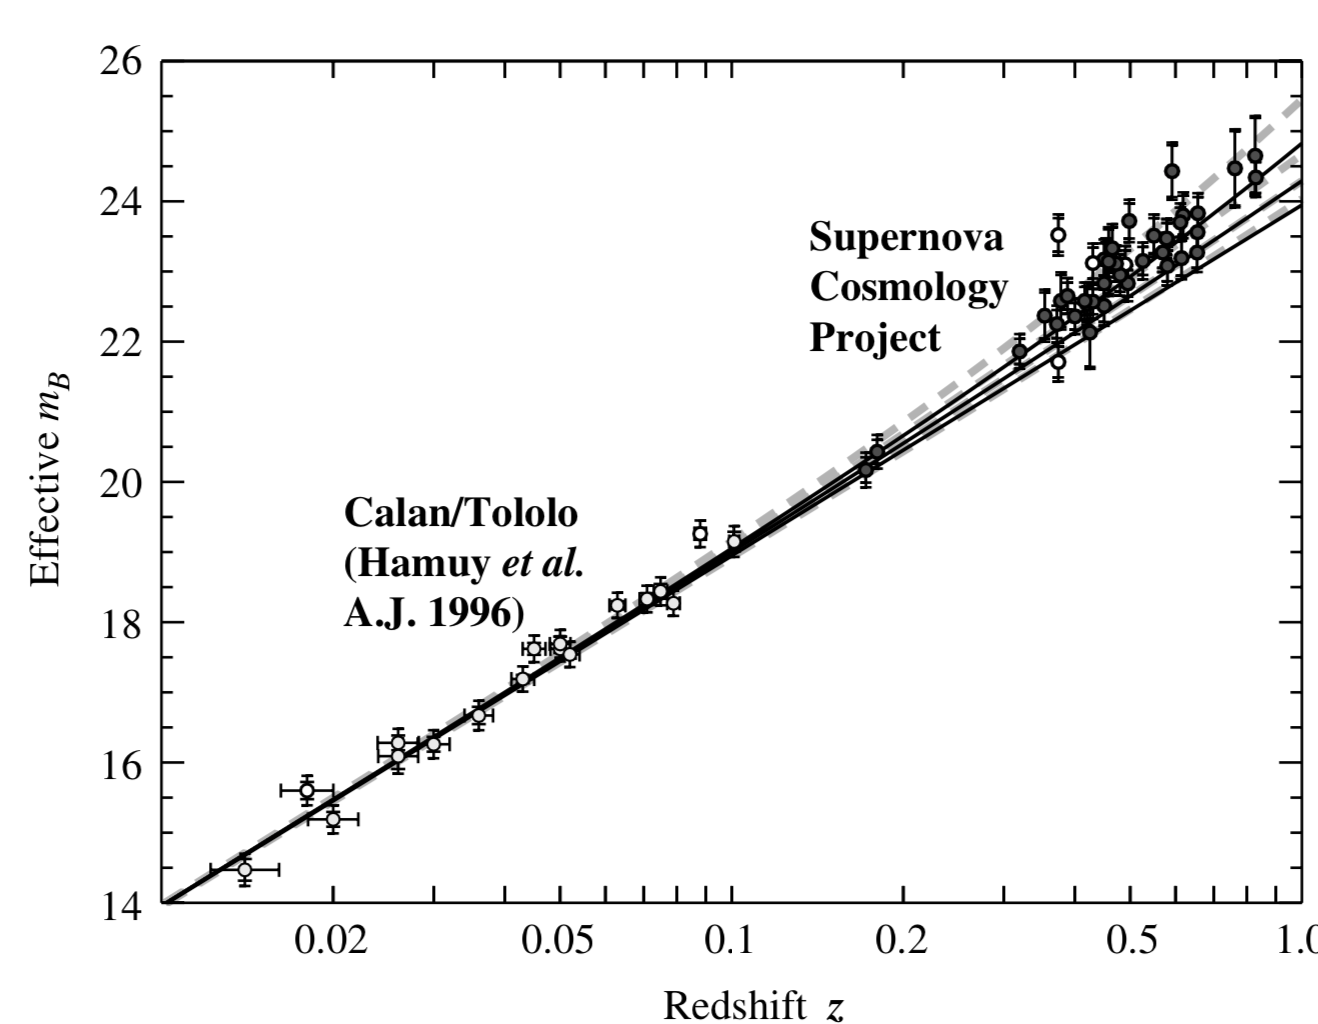
\includegraphics[width=10cm]{figure/fig1-1}
	\label{fig:1-1}
	\caption{}
\end{figure}%

高赤方偏移超新星探査チームの結果が図\ref{fig:1-2}にある。
\begin{figure}[h]
	\centering
	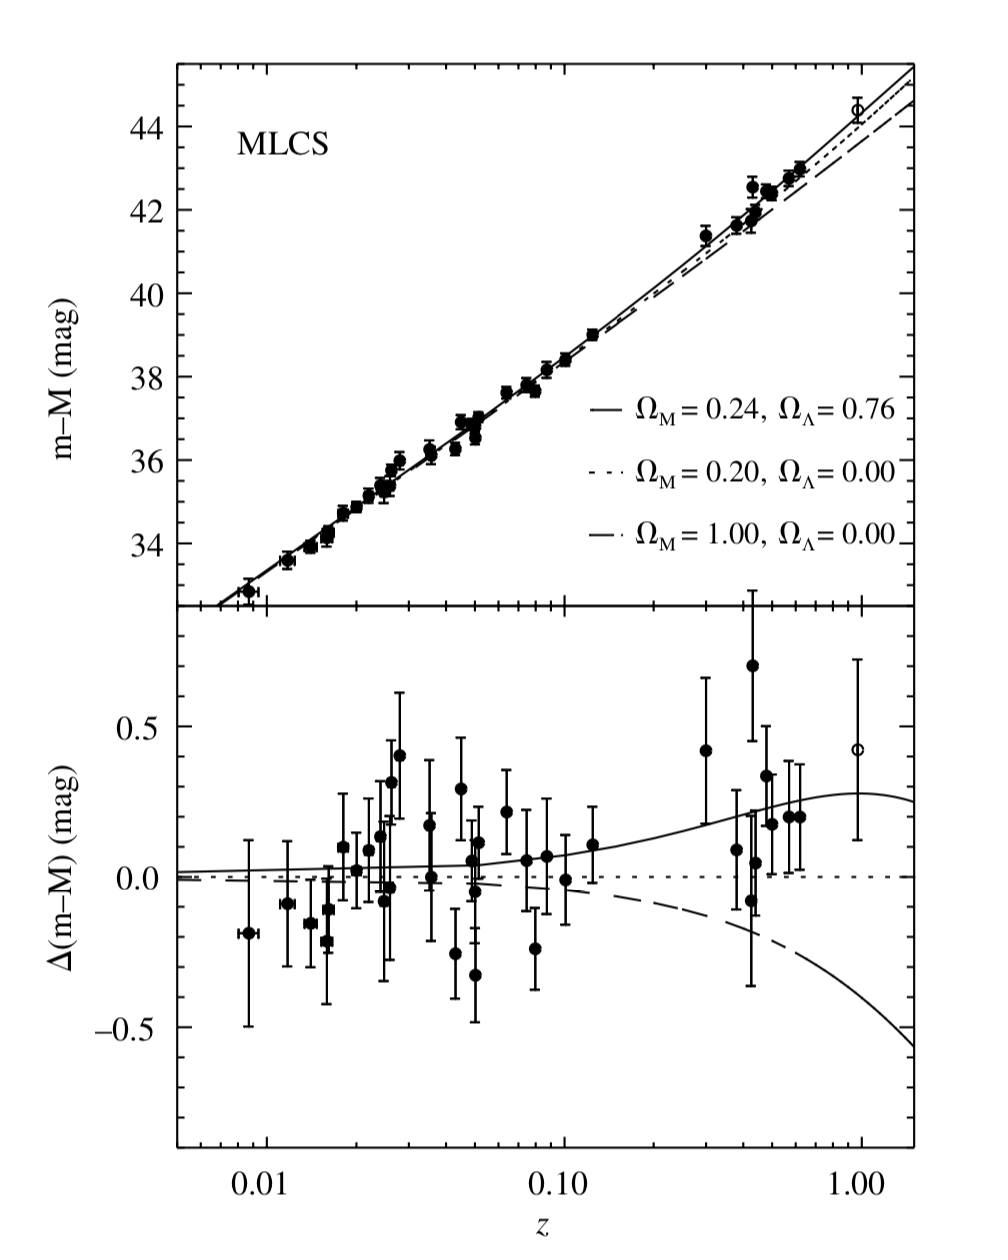
\includegraphics[width=10cm]{figure/fig1-2}
	\label{fig:1-2}
	\caption{}
\end{figure}%
空間の曲率の仮定によらず、99.7\%の信頼度で$\Omega_{\Lambda} > 0$と結論した。
平坦な宇宙モデルにおける最良適合値は$\Omega_{M}=0.28 \pm 0.10 $と$\Omega_{\Lambda}=1-\Omega_{M}$で宇宙年齢は、$(14.2\pm1.5)\times 10^ 9 \,y$である。
$\Omega_{M} \geq 0$のみを仮定し、より自由度の多い光度曲線のモデルを用いて、彼らは、99.5\%の信頼度で$q_0 < 0$と結論した。
すなわち、加速膨張を強く示唆した。

両グループとも$\Omega_{\Lambda}$と$\Omega_{M}$の線型結合を与えることを認識している、とのことだが、なんでこんなことを考えているのか。
というのは、線形結合に現れる”負号”が大事で、物質と真空のエネルギーが宇宙の加速膨張に対しての逆の効果をもたらすことに起因していることが大事。
物質は膨張を減速させて、正の真空エネルギーは膨張を加速させる。($q_0 = (\Omega_{M} - 2 \Omega_{\Lambda} + 2 \Omega_{R})/2$)
例えば、
超新星宇宙論プロジェクトでは、$0.8\Omega_{M} -  0.6  \Omega_{\Lambda}$、
高赤方偏移超新星探査チームでは、$\Omega_{M} -  \Omega_{\Lambda}$やら、$1.4 \Omega_{M} -   \Omega_{\Lambda}$である。
これらの線型結合に現れる負号は真空のエネルギーのように振る舞うエネルギー成分の存在を示していて、この成分は\textgt{ダークエネルギー}と呼ばれている。
余談だが、宇宙論的距離にあるIa 型超新星の観測を$q_0$の測定だとみなすのは正しくない。

次に、高赤方偏移超新星探査チームは、超新星を見つけてその時間発展をおったりして、最良適合値を得た。

さて、少しデータの特徴について。
$\Omega_{\Lambda} > \Omega_{M}$を示す超新星のデータの重要な特徴は、Ia 型超新星の見かけの光度が赤方偏移とともに減少するスピードがアインシュタイン-ド・ジッターモデル($\Omega_{M}=1 , \, \Omega_{\Lambda}  = 0$)で期待されるものよりも早いことである。
真空エネルギーが見かけの光度に及ぼす効果は、真空エネルギーが優勢な平坦な宇宙と、空っぽの宇宙、二つの極端な宇宙モデルで計算された光度距離を比較することによって、調べられる。
\begin{align}
  d_{L}(z)=&\frac{z+z^{2}}{H_{0}} \quad \text { (vacuum dominated) } \\
  d_{L}(z)=&\frac{z+z^{2} / 2}{H_{0}} \quad(\text {empty})
\end{align}%
まあ明らかに、真空エネルギーは全ての$z$において光度距離を増加させるように働くことがわかる。(図\ref{fig:1-3})
\begin{figure}[h]
	\centering
	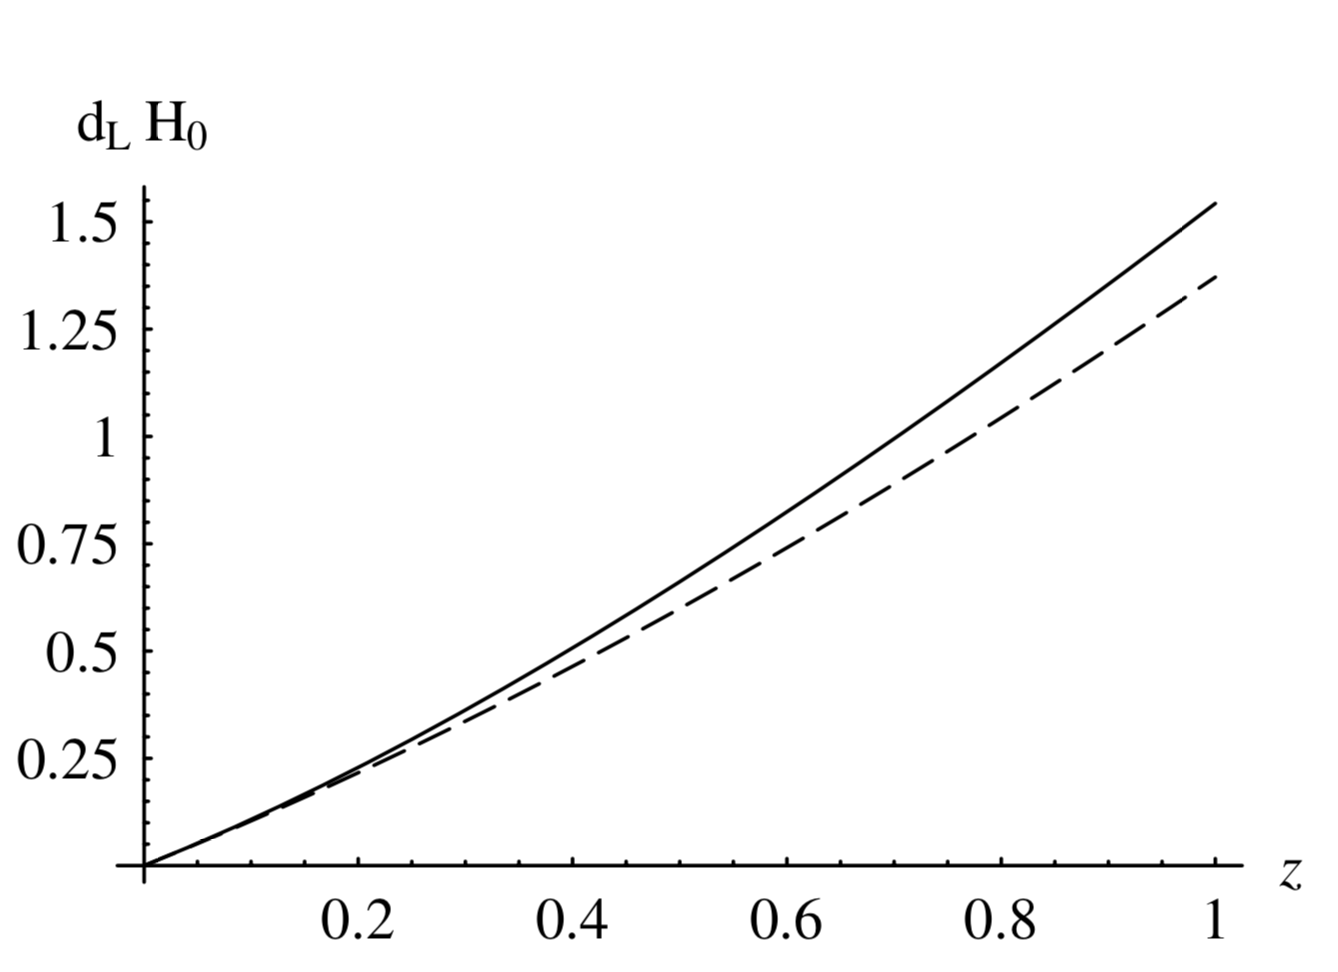
\includegraphics[width=10cm]{figure/fig1-3}
	\label{fig:1-3}
	\caption{}
\end{figure}%

両方のチームともに、彼らが測定した光度距離とIa 型超新星の赤方偏移の関係が真空エネルギー優勢の宇宙の関係に近いことを発見した。
この事実は、宇宙膨張が物質に支配されていて、そこそこ大きい赤方偏移の見かけの光度が$q_0=0$の場合に比べて大きい、という従来の期待と反するものだった。
$q_0$の定義に$-$がついている理由は、この予想のために正の値をとるようにしていたためである。

加速膨張と見かけ光度の現象の関係はどのように理解できるかというと、1.5節でやたニュートン的な宇宙モデルに基づいて議論ができる。

まあ、見かけの光度の現象が加速膨張じゃなくて、光源と僕らの間に介在する物質による光の吸収、散乱で生じている可能性はある。
そのような効果は、その結果に生じる見かけの色なるもの変化を考えればよく、色を慎重に測定することによって解決できる。
しかしながら、簡単ではない。
色を変えずに、見かけの光度を減らすなんらかの銀河間媒体(グレイダスト)を考えることは可能。

この問題は、ハッブル深宇宙探査(Hubble Deep Field)の領域中にある赤方偏移$z = 1.7 \pm 0.1$の銀河で発見された超新星SN1997ffの研究と、新しくできた「より高赤方偏移の」超新星チーム(Higher-z Supernova Team)が発見した新しいIa 型超新星の解析によって解決されている。(ので、心配ない。)
図\ref{fig:1-4}はそれを表していて、二つの宇宙モデルから計算された光度距離の差を表している。
\begin{figure}[h]
	\centering
	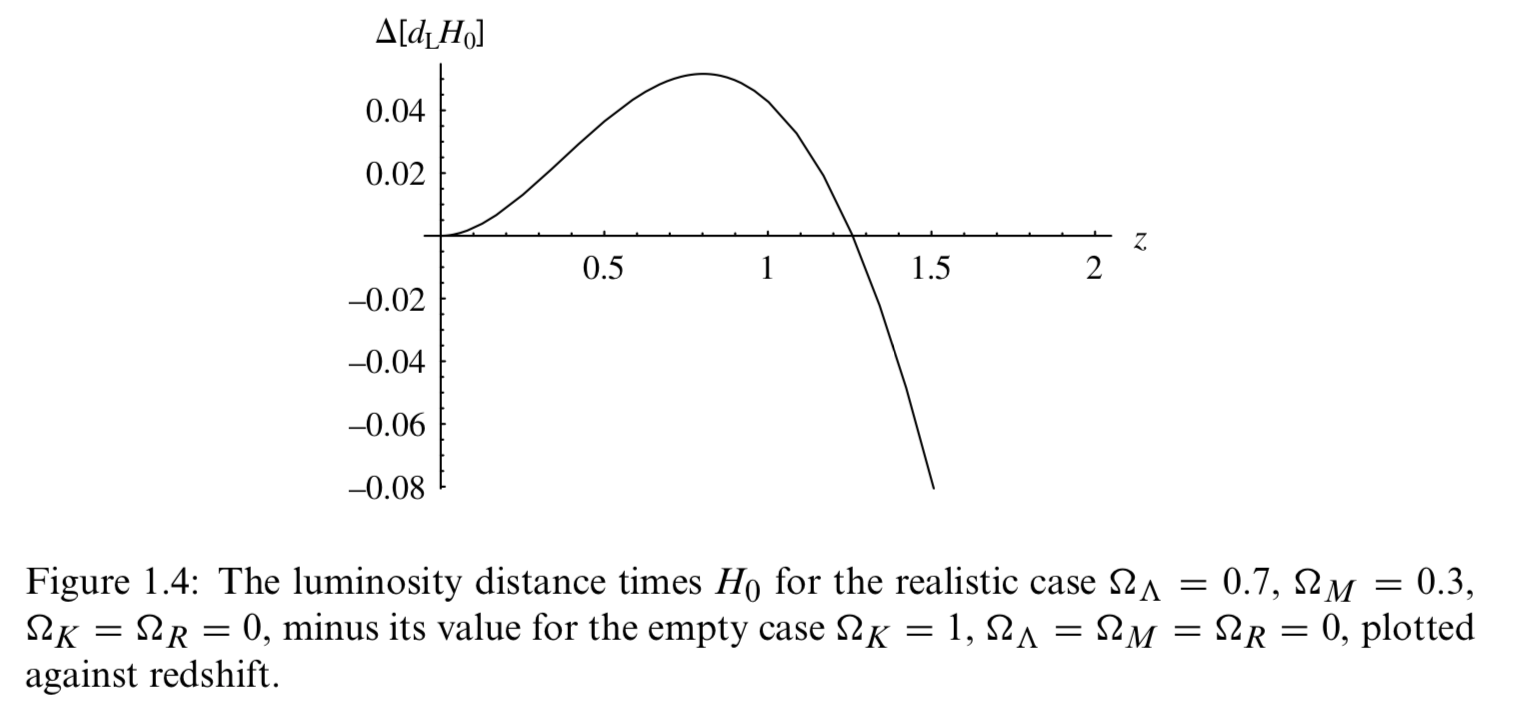
\includegraphics[width=10cm]{figure/fig1-4}
	\label{fig:1-4}
	\caption{}
\end{figure}%
あまりわからないが説明しておくと、
高赤方偏移において、
超新星から放たれた光が僕らに向かって飛んできている時間の大部分は物質が優勢である。
したがって、その頃の宇宙膨張は減速しているはず。
これらの新しい超新星の見かけの光度は、光度距離と赤方偏移の間に線形関係を仮定していたけれども、これより大きいはずであり、光の吸収や散乱では説明ができない。
図\ref{fig:1-4}をみると、$z>1.25$では観測結果を説明する。
グレイダスト、$\Omega_{\Lambda} = 0$から期待される結果とは矛盾。
これらの結論は、ハッブル望遠鏡を用いた、赤方偏移が$0.5$程度のIa 型超新星の光度距離の測定によってさらに強化されて、
物質優勢期から真空エネルギー優勢期への移行に関するさらなる証拠が与えられ、さらにこれから、$z>1$における圧力とエネルギー密度の比が$-1$と無矛盾であること、その時間変化が早くないことが示された。

さて、実はもう一つ深刻な問題があって、Ia 型超新星の絶対光度が、超新星の起こる時期に依存する可能性があるということである。
だが、銀河の場合、遠方にあるほど早期の姿を見ていることになるので、超新星の光度に対する進化の効果は、銀河全体に対するものほど重要ではないと思われる。\footnote{少し曖昧}
例えそうであっても、Ia 型超新星の絶対光度は超新星の元となる二つの星の化学組成に影響を受け、そしてそれは親銀河の進化に影響されるので、そのような効果は超新星の絶対光度と減光時間、および絶対光度と本来の色との間の相関を考慮することで減らすことができるそうだ。

他にひょっとすると、超新星の見かけの光度と赤方偏移の関係に寄与するかもしれない影響は、
\begin{enumerate}
\item 弱い重力レンズ効果。これは非常に小さい領域のみを観測しているので小さいと考えられている。SN1997fの見かけの光度は重力レンズによって増光されていて云々、というお話があったけれども、結果的には重力レンズの効果は小さいと報告された。
\item 宇宙の物質分布の非一様性によって加速膨張が生じるというお話がある。が、十分に大きな空間スケールで平均化した宇宙が高精度で一様であるから、これもありそうにないでしょ、と思われている。
\item 測定の精度を悪くする不訂正。というのは観測所はいっぱいあるから。それらの観測所間の結果を比較する際に様々な較正誤差が生じる可能性。これは実験で頑張るしかない。人の手によるもの。
\item 測定器が限られた波長領域のみに感度があるという問題。これは歴史的に、高赤方偏移における光度距離の測定を難しくしてきた。
宇宙論的赤方偏移は光源の見かけ色を変えてしまうために、見かけの光度が測定される感度を変えてしまう。
これを考慮するために、いわゆるK 補正(K-correction)を用いて、観測された見かけの等級は較正される。
これは暗黒エネルギー発見前に導かれていおり、以後、改良されている。
\end{enumerate}%

さて、これらの加速膨張の観測から得られることは、定数である真空のエネルギーの存在と無矛盾であるが、このエネルギー密度が本当に定数であるか、ということの証明にはなっていない。
加速膨張は$3\ddot{a}/a = \rho + 3 p < 0$であることを要請するが、それは通常の物質や放射ではあり得ない。この成分が暗黒エネルギー(dark energy)と呼ばれる所以である。

暗黒エネルギーが定数でないという可能性は捨てきれていないので、実験では、暗黒エネルギーの圧力とエネルギー密度の比として観測データを解析するのが慣例となっている。
この比$w$が時間変化しない理由はない。
それでも、$w$が定数であるが、必ずしも$-1$に等しくない宇宙モデルはよく調べられている。\footnote{りゆうは?}
暗黒エネルギー密度と、$\Omega_{K}$が負でなければ、宇宙は継続して膨張し続ける。
この場合の暗黒エネルギーの密度は$a^{-3 -3w}$のように変化する。

もし、$w <0$であれば、十分時間が経過すると、最終的に、放射と物質のエネルギー密度は暗黒エネルギー密度と比べて無視できうるほど小さくならなければならない。
もし、$w,<1/3$であれば、フリードマン方程式における空間曲率の効果も最終的には無視できるようになる。
$-1<w$かつ$\dot{a}>0$の場合、解は$t  \to Ca^{(3+3w)/2} + t_1$となる。
もし、$w<-1$かつ$\dot{a}>0$の場合の解は、$a$が時刻$t_1$において無限大になるという特筆すべき性質を持つ。これはしばしばファントムエネルギー(phantom energy)と呼ばれる。この場合は、$w,\geq -1$の場合と異なり、全ての構造は最終的には暗黒エネルギーに付随する赤緑によって引き裂かれてしまう。\footnote{なんかかっこいい。}

2003年、カナダ-フランス-ハワイ望遠鏡で開始された調査(Supernova Legacy Survey)があって、それと、ESSENCEで得られたデータから、$w=-1.07 \pm 0.09(\text { stat }, 1 \sigma) \pm 0.13(\text { syst }), \quad \Omega_{M}=0.267_{-0.018}^{+0.028}(\text { stat }, 1 \sigma)$という結果を得た。

実は、暗黒エネルギーが宇宙のエネルギー密度の大部分を占めているという結論は、宇宙マイクロ背景放射の観測で確認されている。これは7.2節でのお楽しみ。
また、X線の観測からも支持されている。これは銀河団の高温ガスから発せられる。

バースト時間の長い長期型のガンマ線バーストを2次の距離指標として用いることで、光度距離の測定をさらに高赤方偏移まで伸ばすことができるかもしれない。
ガンマ線バーストは、一定の絶対光度を持っていないけれども、その絶対光度が、見かけの光度が最大となるエネルギーおよび特徴的な時間スケールと相関を持つという示唆があるからだ。

暗黒エネルギーの発見は、(もちろん他の観測の解釈の上で重要だけど)基礎物理に対する挑戦という意味において非常に重要である。
暗黒エネルギーの密度がなぜこんなにも小さい値をとるのか?というのが最も大きな問題である。\footnote{これもなんかかっこいい}

\newpage
\setcounter{section}{9}
\setcounter{page}{1}
\section{銀河間のガスによる吸収(Intergalactic absorption)}\label{sec1-10:Intergalactic-absorption}

最初の銀河および銀河団の元となった原子核や電子ガスの一部は、全て銀河になったわけではなく、銀河間の空間に残っている。
%これを考えると、銀河の元になっているわけであるからその素材部分がわかれば嬉しいでしょう、ということ。
本節では、この銀河間(intergalatic)にある原子核や電子からなるガス(銀河間ガス)について考える。
\footnote{用語の説明。Wikipediaによれば、銀河間ガス、銀河団ガス、と二つあるらしい。
銀河団ガス(ぎんがだんがす、Intracluster medium;ICM)は銀河団内を満たす高温のガスのことである。
銀河間ガス(ぎんがかんがす、Intergalactic Medium;IGM)は、銀河団ガスと同様の意味で使われることもあるが、多くの場合、銀河団より外に存在するガスのことを指すとのことである。
本文では、intergalatic とあるので、銀河間ガスとこのノートで書いたけれど、Wienberg は特に区別して使っているわけではないと思う。
}
ガス中の原子や分子は観測可能で、より遠方にある銀河やクエーサー(quasar)
\footnote{これは、94ページで出てきた新しい単語で、Wikipedia によると、「クエーサー(英: Quasar)は、非常に離れた距離に存在し極めて明るく輝いているために、光学望遠鏡では内部構造が見えず、恒星のような点光源に見える天体のこと。クエーサーという語は準恒星状(quasi-stellar)の短縮形である。日本語ではかつて準星などと呼ばれていた。」とのこと。いろいろと面白い話がありそう。この節で関係ありそうなところを書いておくと、「$ 0.16 <z <7$ 付近に発見されている。観測されるクエーサーは非常に暗いが、これだけ大きな赤方偏移を生じるほど遠方にあることから、実際にはクエーサーは宇宙に存在する天体の中で最も明るいと考えられている。一般的にクエーサーの明るさは $10^{38}$ W(最も明るい電波銀河の光度)から $10^{42}$ W に達」するとある。}
からやってくる光または電波の共鳴吸収%\footnote{これは、あまりわからない。}
によって観測できるであろう。%\footnote{could}
しかし、ガスの大部分は(今はもうない)高温で質量の大きい第一世代の星(first generation of hot massive stars)の光で電離してしまったと信じられている。%\footnote{believed}
なお、その星は、とうの昔に寿命が尽きて無くなっており、時々、種族III(Population III)の星と呼ばれている。
%\footnote{関係詞。}
現在のところ、一部のクエーサーは宇宙のガスの電離が完了する前に形成されたと思われており、%\footnote{now appear}、
非常に遠方%\footnote{早期という意味。}
からの光の共鳴吸収を用いれば、銀河間ガスを測定できる可能性がある。

原子の遷移によって、遠方の光源が光線を放射して、
時刻$t_1$に周波数$\nu_1$で放射され、時刻$t_0$に周波数$\nu_0$で地球に届いたとする。
この光が到達するまでに、ある時刻$t \, (t_1 <t< t_0)$における周波数は、赤方偏移の因子ががかって、$v_{1} a\left(t_{1}\right) / a(t)$となっている。
\footnote{式(1.2.3)を思い出すと、$\delta t_1 /a(t_1) = \delta t_2 /a(t_2)$から出せるのだった。}
もし、銀河間ガスが周波数$\nu$の光を単位時間当たりに$\Lambda(\nu,t)$ので、割合で吸収し、かつ光を放出しないとすれば、この光線の光の強度は次の方程式:
\begin{align}
 \dot{I}(t)=-\Lambda\left( \nu_{1}  \frac{a \left(t_{1}\right) }{ a(t)}, t\right) I(t)
\end{align}%
に従う。
もし銀河間ガスが温度$T(t)$を持っていれば、誘導放射によってこの光線に同じ周波数で、同じ位相で、同じ偏光を持った光子が加えられる。
この光子一個当たりの誘導放射率は、アインシュタインの公式:$\exp(-h \nu/k_B T)$の因子で与えられて、この修正を方程式に施せば、
\begin{align}
  \dot{I}(t)
  =-\left[1-\exp \left(-\frac{h \nu_{1} a\left(t_{1}\right)}{k_{\mathcal{B}} T(t) a(t)}\right)\right] \Lambda\left( \nu_{1}  \frac{a \left(t_{1}\right) }{ a(t)}, t\right)  I(t)
\end{align}%
となる。これより、地球で観測される周波数は、
\begin{align}
  I\left(t_{0}\right)=\exp (-\tau) I\left(t_{1}\right)
\end{align}%
となる。ここで、$\tau$は光学的厚さ(optical depth)と呼ばれている。
\begin{align}
 \tau = \int_{t_1}^{t_0} dt  \left[1-\exp \left(-\frac{h \nu_{1} a\left(t_{1}\right)}{k_{\mathcal{B}} T(t) a(t)}\right)\right] \Lambda\left( \nu_{1}  \frac{a \left(t_{1}\right) }{ a(t)}, t\right) 
\end{align}%
吸収率は、
\begin{align}
  \Lambda(v, t)=n(t) \sigma(\nu)
\end{align}%
で与えられる。
ここで、
$\sigma(\nu)$は周波数$\nu$における吸収断面積で、
$n(t)$は単位体積あたりの吸収をになう原子の数密度である。
多くの場合、$\sigma(\nu)$はある$\nu_{R}$で鋭いピークを持つ。
したがって、吸収は、周波数$\nu_{R}$に対応する時刻$t_R$に近い時のみにおこり、その
$t_R$は、
\begin{align}
  a\left(t_{R}\right)=\nu_{1} a\left(t_{1}\right) / \nu_{R}
\end{align}%
と与えられる。
ゆえに、光学的厚さ$\tau$は、
\begin{align}
  \tau \simeq n\left(t_{R}\right)\left[1-\exp \left(-h \nu_{R} / k_{\mathcal{B}} T\left(t_{R}\right)\right)\right] \int \sigma\left(\nu_{1} a\left(t_{1}\right) / a(t)\right) d t
\end{align}%
近似できる。これを、$\nu(t) = \nu_{1} a(t_1) / a(t)$を用いて、積分変数を時間から周波数に書き換えて、主な寄与がピーク付近$\nu_{R} ( \leftrightarrow t_{R})$であることを考慮すれば、次の公式:
\begin{align}
  \tau \simeq n\left(t_{R}\right)\left[1-\exp \left(-h \nu_{R} / k_{\mathcal{B}} T\left(t_{R}\right)\right)\right]\left[a\left(t_{R}\right) / \dot{a}\left(t_{R}\right)\right] \mathcal{I}_{R}  \,,\quad  (\mathcal{I}_{R} \equiv \frac{1}{\nu_{R}} \int \sigma(\nu) d \nu) \label{eq:1.10.6}
\end{align}%
が得られる。積分範囲は、ピークを含む狭い周波数領域。
この$\tau$の式を眺めてみると、唯一、宇宙論モデルに依存するのは、吸収の時刻における宇宙膨張率(ハッブル定数)$\dot{a}(t_R) / a(t_R)$であり、それは、
\begin{align}
  \frac{\dot{a}\left(t_{R}\right)}{a\left(t_{R}\right)}=H_{0} \sqrt{\Omega_{\Lambda}+\Omega_{K}\left(1+z_{R}\right)^{2}+\Omega_{M}\left(1+z_{R}\right)^{3}+\Omega_{R}\left(1+z_{R}\right)^{4}}
\end{align}%
で与えられる。(式(1.5.41)で、時刻$t \rightarrow t_R$とすればでる。)
ここで、$z_{R} (=a\left(t_{0}\right) / a\left(t_{R}\right)-1=\nu_{R} / \nu_{0}-1)$は、共鳴吸収が起こる場所での赤方偏移である。
ある赤方偏移$z$に対して、吸収は観測される周波数$\nu_0 = \nu_1/(1+z)$のうちある決まった領域に渡って起こり、その領域は、$t_R$が$t_1$と$t_0$の間にあるという条件$:t_1<t<t_0$と$a(t)$が増加関数であることから求まる。\footnote{$t_1 \leq t_R$から$a(t_1)/a(t_R) \leq 1$で両辺に$\nu_0$をかけたら$\nu_{R} /(1+z) \leq v_{0} $が出て、もう一方は$a(t_R) \leq a(t)$を、直前と同様に逆数とればでる。}
\begin{align}
  \nu_{R} /(1+z) \leq v_{0} \leq \nu_{R} \label{eq:1.10.9}
\end{align}%

次に、歴史(例)を見てみる。
1959年、Field は、水素原子の21 cm 線の遷移による電波の吸収の効果を観測することを提案した。
このスペクトル線は、水素の1s 状態における超微細構造がスピン0からスピン1のエネルギー分裂によるものである。\footnote{21 cm 吸収線は、Secondary distance のTally-Fisher 関係でも活躍した。}
この場合、$\lambda \approx 21 \,\mathrm{cm}$であるから、$1420 \, \mathrm{MHz}$で、赤方偏移$z=0.056$にある銀河、白鳥座A の電波スペクトルは、$1420/(1+0.056) \sim 1345$なので、$1342\,\mathrm{MHz}$から$1420 \, \mathrm{MHz}$の間に式\eqref{eq:1.10.9}から与えられる吸収線の谷を示すはずである。
残念ながら、銀河間の空間の中性水素\footnote{21 cm 吸収線を見ている時点で、中性水素を見ていると仮定している。}の温度は、$h \nu_{R} / k_{\mathcal{B}}=0.068\, \mathrm{K}$よりもはるかに大きいために、式\eqref{eq:1.10.6}で与えられる光学的厚さは$0.068 \, \mathrm{K} / \mathrm{T}\left(t_{R}\right)$の因子だけ小さくなってしまう。(残念ながら)この吸収線の谷の兆候は未だに発見されていない。
将来、高角度分解能を持つ新世代の低周波電波望遠鏡を用いることで、高赤方偏移における21 cm 放射の輝線と吸収線を観測して、構造の進化、および構造の種となった原始密度揺らぎを研究できると期待されている。\footnote{大事な動機。}
例えば、2010年までには低周波干渉計
(LOw Frequency ARray (LOFAR)) によって、赤方偏移5から15の間にある光源からの21 cm 照射を高感度、高角度分解能で研究できるはずである、とのこと。
調べてみると、例えば、\href{https://arxiv.org/pdf/1809.06661.pdf}{arXiv:1809.06661}によると、$z = 20-25$の領域で、14 時間ほど測定すれば、21 cm のtemperature fluctuations のpower spectrum の上限が得られるとのこと。\\
%{\mgfamily ここまで。ライマン・アルファ遷移は次にする。}

現在のところ、銀河間の水素原子の性質は、1s の基底状態から2p の励起状態への遷移であるライマン・アルファ遷移の光子の吸収によって詳しく調べられており、ガーン-ピーターソン効果(Gunn–Peterson effect)として知られている。この効果は、1965年の論文で出た。
吸収の観測は、昔から調べられているようだ。
この遷移は、紫外線領域に共鳴周波数$\nu_{R} = 2.47 \times 10^{15} \, \mathrm{Hz}$を持ち、それは波長1,215 {\AA}に対応する。
しかし、赤方偏移が$z>1.5$にある光源に対しては、式\eqref{eq:1.10.9}から、吸収線の谷の低周波数の極限が波長3,000{\AA}よりも長くなる($吸収線の谷の低周波数の極限\,c/(\nu_{R}/(1+z)) > 3,036 \,\text{{\AA}}$)。
これより、可視光や赤外線部分のスペクトルを用いて地上から観測することができる。
ライマン・アルファ線は$h \nu_{R} / k_{\mathcal{B}}=118,000\, \mathrm{K}$であり、これは大抵の場合、銀河間ガスの温度よりも高い。
したがって、式\eqref{eq:1.10.6}の因子を$\exp \left(-h \nu_{R} / k_{\mathcal{B}} T\left(t_{R}\right)\right) \sim 0$とすることができて、
また、積分$\mathcal{I}_{R}$は、$1/(4.5 \times 10^{-18} \, \mathrm{cm^2})$の値を持つから\footnote{これはどこかの実験値で決めてきたんだと思う。}、式\eqref{eq:1.10.9}で与えられる吸収線の谷の低周波数極限のすぐ上の周波数における光学的厚さは、
\begin{align}
  \tau_{\nu_{0}=\nu_{R} /(1+z)+}=\left(\frac{n\left(t_{R}\right)}{2.4 h \times 10^{-11} \mathrm{cm}^{-3}}\right)\left(\Omega_{\Lambda}+\Omega_{K}(1+z_R)^{2}\right.+\Omega_{M}(1+z_R)^{3}+\Omega_{R}(1+z_R)^{4} )^{-1 / 2}  \label{eq:1.10.10}
\end{align}%
で与えられる。

宇宙のバリオンの中に銀河間中性水素原子が少しだけ存在するような状況を考えてみる。
例えば、もし、宇宙のバリオンの中の一部$f$が、$z=5$に対応する時刻において、銀河間の中性水素原子にあったとすれば、$\Omega_{B} h^{2}=0.02$のとき、$z = 5$における水素原子の数密度は$4.8 f \times 10^{-5}$である。
これは、赤方偏移$z$を考慮してバリオンの質量密度を出して、バリオンを代表して陽子の質量で割ったもの、すなわちバリオンの数密度に、$f$をかけたもの:
\begin{align}
(1+z_R)^3  \frac{\Omega_{B} \rho_{\text{crit}}}{m_p} f 
   = \frac{0.02/h^2 \times 1.878h^2 \times 10^{-29} \, \mathrm{g/cm^3} \times (1+5)^3 f}{1.67262171(29) \times 10^{-24} \,\mathrm{g}} \approx 4.850 f  \times 10^{-5} \, \mathrm{/cm^3}
\end{align}%
から計算した。
宇宙論パラメータとして$h=0.65, \Omega_{\Lambda}=0.7, \Omega_{M}=0.3, \, \Omega_{K}=\Omega_{R}=0$を選べば、光学的厚さは、式\eqref{eq:1.10.10}から$3.8 f \times 10^{5} $とわかる(代入したら出る)。
したがって、これらのパラメータに対しては、宇宙のバリオン物質の量に対する比$f \gg 2.6 \times 10^{-6}$である場合、吸収線の谷の低周波数極限のすぐ上の周波数における光学的厚さは、$3.8 f\times 10^5 \gg 0.988 \sim 1$となるので、強度は$1/e$以下。
したがって、銀河間の中性水素は$z=5$を超える光源からの赤方偏移を受けたライマン・アルファ線より高い周波数を持ついかなる光も完全に吸収してしまうことがわかる。

少し観測の歴史の昔話。ハッピーエンドで終わるので気楽に読むのが大事。
長年にわたって、ライマン・アルファ吸収線の谷の探索は失敗に終わっていた。
クエーサーのスペクトルは膨大なライマン・アルファ吸収線を示していたけれども、それらは、通常「ライマン・アルファの森(Lyman α forests)」と呼ばれていて、視線方向に存在する中性水素の雲から生じると考えられている。
しかし、$z \approx 5$までにあるクエーサーのスペクトルには、上述のような状況、すなわち、たとえ宇宙のバリオンのごくわずかな割合$f$だけでも中性水素原子であったとすれば、赤方偏移を受けたライマン・アルファ線より高周波側に見られるだろう一様な光の減衰は発見されなかった。
これが1999年。
時は2001年、ついに完全な光の減衰の兆候が見つかった。
スローン・デジタル・スカイサーベイによって発見された赤方偏移$z =6.28$のクエーサー SDSSp J103027.10+052455.0のスペクトル中に赤方偏移を受けたライマン・アルファ線の波長8845\,{\AA}よりすぐ短波長側から8450\,{\AA}にかけて、一様な光の減衰が観測された(図\ref{fig:1-8})。
\begin{figure}[H]
\centering
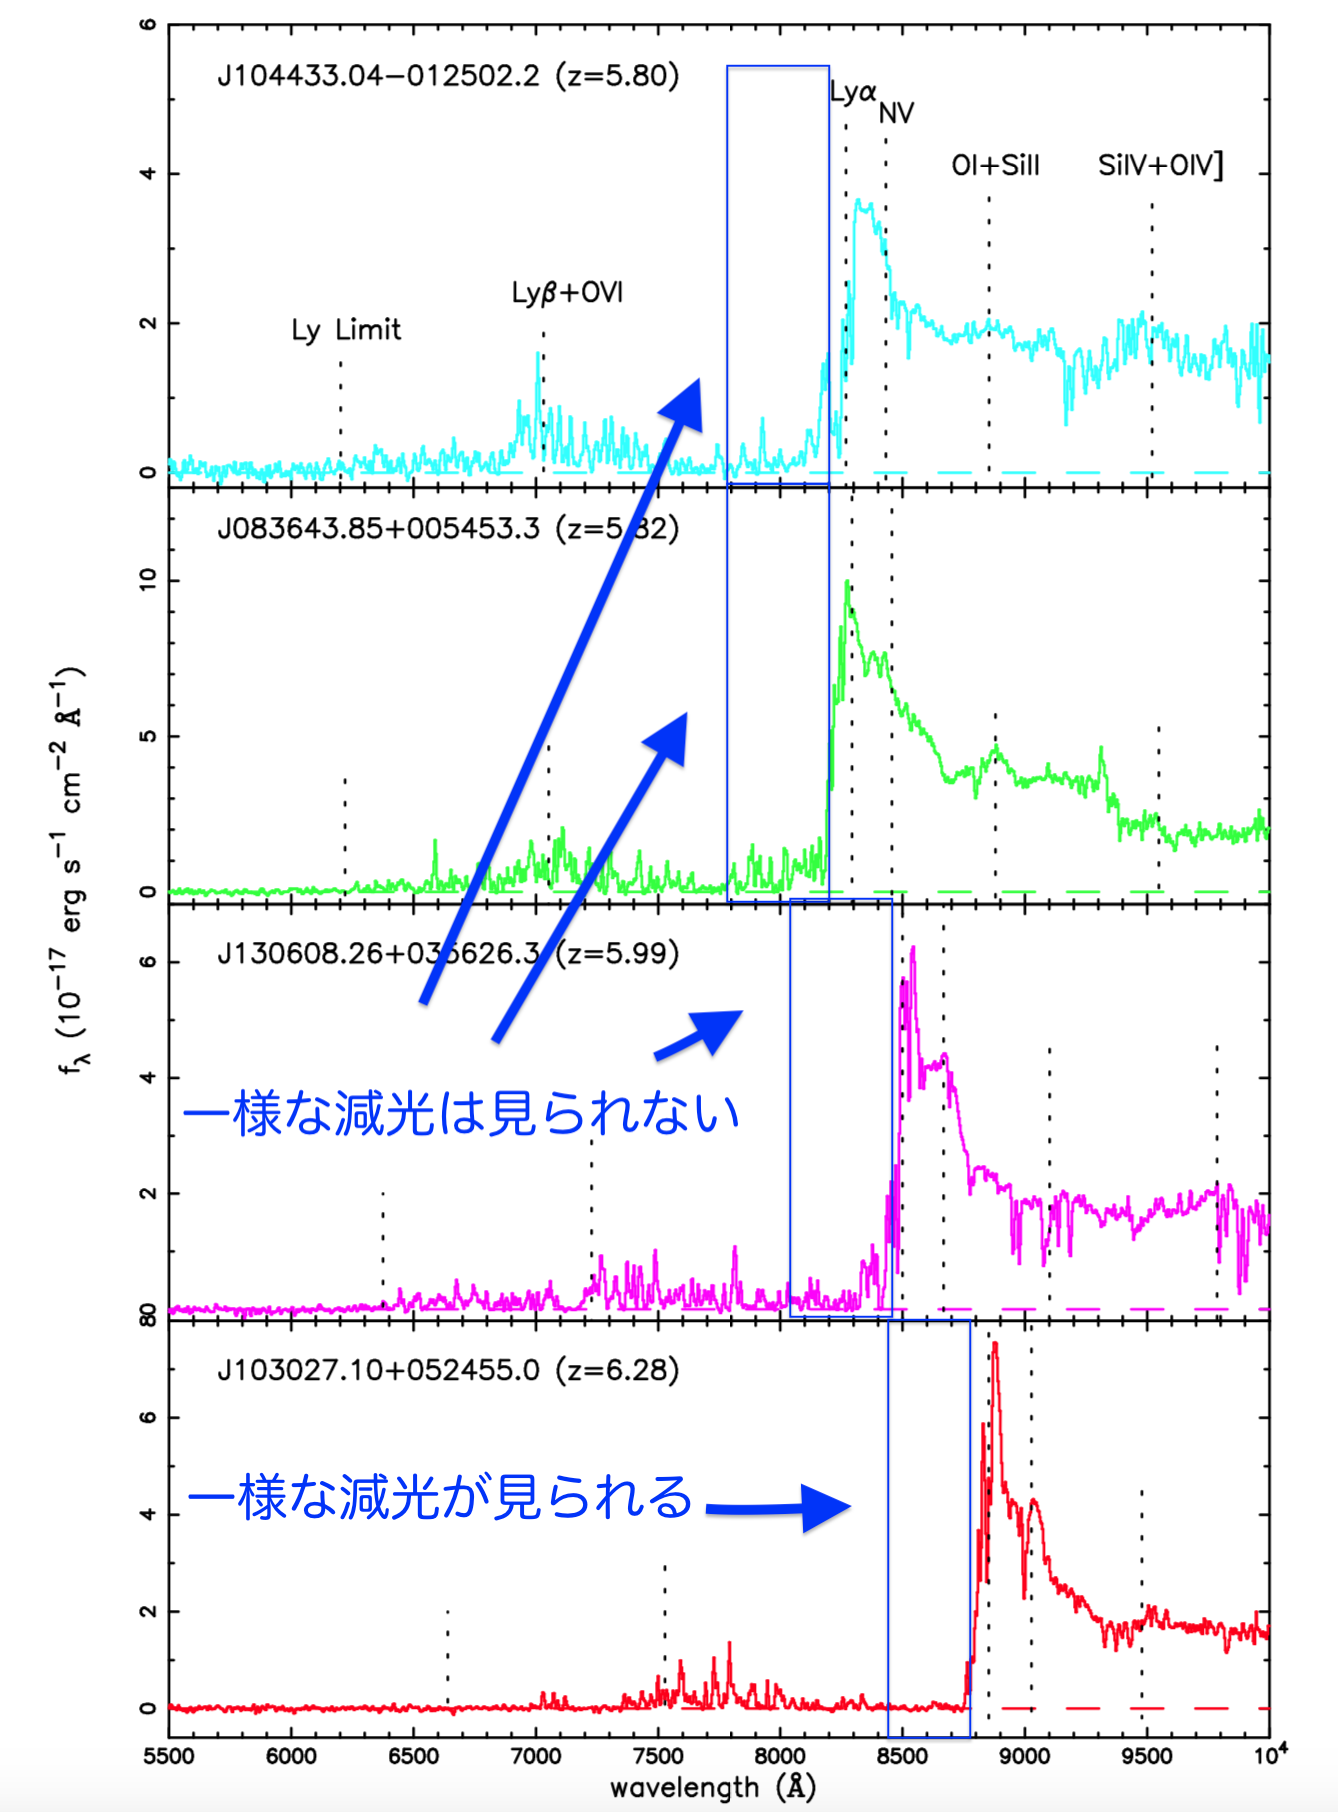
\includegraphics[width=13cm]{figure/fig1-8}
\label{fig:1-8}
\centering
\caption{高赤方偏移にある4つのクエーサーから観測された光の強度を波長に対してプロットしたグラフである。\footnote{なお、S/N比をよくするために、図の1ピクセルが4{\AA}とされているらしい。}
([\href{https://arxiv.org/abs/astro-ph/0108097}{arXiv:astro-ph/0108097}のFigure 1])
破線は、赤方偏移を受けて予想される様々なスペクトル線の波長を示している。
$z=6.28$のクエーサーの方向では、8845\,{\AA}にあるライマン・アルファ線のすぐ左で光の強度が実験の制度の範囲内で0まで落ちている。
これは、他の$z = 5.80,5.82,5.99$のクエーサーには見られない現象である。
これは、ほぼ完全に電離している領域が赤方偏移$z = 5.99 から 6.28$の間で現れたことを示している。
}%
\end{figure}%}
\newpage
したがって、$z=6$のあたりで「暗黒時代」が終わったのかもしれない。
というのは、暗黒時代の宇宙空間は中性水素原子による光の吸収のため、赤方偏移を受けたライマンアルファ線の周波数より高い周波数の光に対して不透明なのである。
この結論に対するさらなる証拠もあって、高赤方偏移で生じたガンマ線バーストとして知られる強烈なガンマ線光源のスペクトルから得られている。

余談だが、近年、重力波の観測成功により、マルチメッセンジャー天文学が本格的に幕開けしたという話がある。
マルチメッセンジャー天文学というのは、従来の光(X線やガンマ線、赤外線も含む)だけでなく複数の手段によって天体の観測をするということ。
PRLの\href{https://twitter.com/PhysRevLett/status/919925957573582848}{このツイート}の\href{https://journals.aps.org/prl/abstract/10.1103/PhysRevLett.119.161101}{この論文}(\href{https://arxiv.org/abs/1710.05832}{arXiv:1710.05832})によると、LIGO-Virgoが連星中性子星の合体イベントからの重力波を捕えて、ガンマ線観測用の天文衛星フェルミもガンマ線バーストを同時観測し、またその報告を受けた多くの光学望遠鏡による追観測も行われたそうだ。
今回の観測によって、(ショート)ガンマ線バーストと連星中性子星の合体が初めて直接関連付けられ、また、連星中性子星の合体で生じると予想されていた巨新星(キロノヴァ)も光学望遠鏡の追観測によって初めて観測されたとのこと。
なんかすごい時代に突入しているということは僕みたいな素人でも伝わってくる。

話を戻して、上の(さらに上の)観測結果だけでは、$z>6$の宇宙における全ての水素はおろか、そのほとんどが水素原子だとことを意味しない。
というのは、ほんのわずかな水素の割合($f \gg 2.6 \times 10^{-6}$)があっただけでも、遠方クエーサーのスペクトルに吸収線の谷ができるのであった。
実際、現在では、7章で見るように宇宙マイクロ波背景放射の研究から、水素は$z\approx 6$よりもっと大きな赤方偏移では、(おそらく$z \approx 10$において)すでにほとんど電離しているという証拠が上がっている。

ライマン・アルファの森を形成している、$z<6$にある中性水素の雲を使えば、他の手法とは独立に$\Omega_{m}$と$\Omega_{\Lambda}$を決めることができる。
このアイデアは、1979年のアルコック-バチンスキー(Alcock–Paczyn ́ski)の論文にまで遡る。
ある赤方偏移$z$にある、広がった光源(object)を観測するとする。
その広がりは、視線方向と垂直な方向と平行な方向で固有距離でそれぞれ$D_{\perp}、D_{\parallel}$としよう。
角径距離(angular diameter distance)の定義によると、この天体(object)は以下の角度をsubtend する。
\begin{align}
  \Delta \theta=D_{\perp} / d_{A}(z)
\end{align}%
また、この天体全体からの光を同時刻$t_0$で観測する際、この天体の視線の奥側と手前側から光が放射された時刻$t_1$の差は$\Delta t_{1} = D_{\parallel}$となる。
赤方偏移は、$a(t_0) / a(t_1) -1 $であるから、この天体の奥側と手前側の赤方偏移の差の絶対値は、
\begin{align}
  \frac{\Delta z}{\Delta \theta} 
    =& \left| - \frac{a(t_0)}{a^2(t_1)} \dot{a}(t_1) \Delta t_1 \right| \\
    =& \underbrace{\frac{a(t_0)}{a(t_1)}}_{=1+z}  \underbrace{\frac{\dot{a}(t_1)}{a(t_1)} }_{=H(z)} \underbrace{\Delta t_1}_{=D_{\parallel}}\\
    =& (1+z)H(z) D_{\parallel}
\end{align}%
で与えられる。$H(z) \equiv \dot{a}\left(t_{1}\right) / a\left(t_{1}\right)$と書いたのは、光が放射された時刻$t_1$でのハッブル定数である。
角径距離$\Delta \theta$と$\Delta z$の比をとる。
\begin{align}
  \frac{\Delta z}{\Delta \theta}=(1+z) H(z) d_{A}(z)\left(D_{ \parallel} / D_{\perp}\right)
\end{align}%
ここで、フリードマン方程式から、
\begin{align}
  \dot{a}^2 + K =& \frac{8\pi G \rho a^2}{3}\\
  \rightarrow 
  \frac{\dot{a}^2}{a^2} =& H_0^2  \left[ \Omega_{\Lambda} + \Omega_{K}\left(\frac{a_0}{a}\right)^2 + \Omega_{M} \left(\frac{a_0}{a}\right)^3 +\Omega_{R} \left(\frac{a_0}{a}\right)^4 \right] 
\end{align}
だった。
また、$d_A(z) = (1+z)^{-2} d_{L} = (1+z)^{-2} a_0 (1+z)r(z)$だったので、
\begin{align}
  d_{A}(z)
    =&\frac{1}{(1+z) H_{0} \Omega_{K}^{1 / 2}} \sinh \left[\Omega_{K}^{1 / 2} \int_{1 /(1+z)}^{1} \frac{d x}{x^{2} \sqrt{\Omega_{\Lambda}+\Omega_{K} x^{-2}+\Omega_{M} x^{-3}+\Omega_{R} x^{-4}}}\right]
\end{align}%
とかけた。これを使えば、現在の時刻のハッブル定数$:H_0$は、$d_A$と$H(z)$のファクタとで打ち消しあうから、
\begin{align}
  \frac{\Delta z}{\Delta \theta}
    =&\left(D_{ \|} / D_{\perp}\right) \Omega_{K}^{-1 / 2} \sqrt{\Omega_{M}(1+z)^{3}+\Omega_{\Lambda}+\Omega_{R}(1+z)^{4}+\Omega_{K}(1+z)^{2}} \\
     &\times \sinh \left[\Omega_{K}^{1 / 2} \int_{1 /(1+z)}^{1} \frac{d x}{x^{2} \sqrt{\Omega_{\Lambda}+\Omega_{K} x^{-2}+\Omega_{M} x^{-3}+\Omega_{R} x^{-4}}}\right]
\end{align}%
と、結局のところ、$H_0$に依存せずに、$z$、$D_{\parallel}/D_{\perp}$、そして、密度パラメータ$\Omega$のみに依存する量になる。
例えば、もし、その観測する天体が球対称の銀河のように、球であるとわかっていたなら、直ちに$D_{ \parallel} / D_{1}=1$である。
そして、$\Delta z$と$\Delta \theta$の測定によって、進化や銀河間の吸収の心配せず、モデルによらずに、$\Omega_{S}$ \footnote{Sは、some という意味だと思う。}への拘束をかけることができる。


だが、不幸にも、高赤方偏移で球対称な天体を見つけることは容易ではない。
しかし、天体の分布が球対称である天体は様々なものがある。
例えば、散在銀河(field galaxies)の分布は、おそらく空間のあらゆる点に関して球対称であろうから、アルコック-バチンスキーの手法を銀河に対して応用することで、宇宙定数の決めることができるかもしれない、ということが提唱されている。
実際、この手法は2度視野クエーサー赤方偏移サーベイ(2dF QSO Redshift Survey)で測定されたクエーサーの分布に応用された。
銀河の代わりにこの方法を用いたわけだが、この観測結果を、$K=0$を仮定して解析すると、$\Omega_{\Lambda}  = 0.71^{+0.09}_{-0.17}$が得られる。


最近、アルコック-バチンスキーのアイデアはライマンアルファ雲の分布関数に適用されている。
すでに議論したように、これらは銀河間に存在する中性水素原子を含む雲であり、視線方向にある遠方のクエーサーからの光を$1\mathrm{s} \to 2\mathrm{p}$の遷移によって吸収する。
雲が赤方偏移$z$にある場合、この吸収線は、クエーサーのスペクトルに波長$1215(1+z)\,\text{\AA}$の暗線として現れる。
さて、様々な方向$\hat{n}$の様々な赤方偏移$z$にあるライマン・アルファ雲の数密度$N(z,\hat{n})$を測定するとしよう。
ライマン・アルファ雲が球対称に分布していると仮定する。
これらの雲の分布関数の$(z,\hat{n})$と$(z+\Delta z, \hat{n} + \Delta \hat{n})$の互いに近い二点における密度関数の積の平均\footnote{二点相関関数みたいなもの}は、$z$と二点間の固有距離のみの関数であり、そして、これら二点間を結ぶベクトルの成分に関して解析的になる。
したがって、
\footnote{
Assuming a spherically symmetric distribution of Lyman α clouds, the mean value of the product of the number densities of these clouds at two nearby points with redshifts z and z + 􏰃z (with 􏰃z ≪ 1) and directions nˆ and nˆ + 􏰃nˆ separated by a small angle 􏰃θ will be a function only of z and the proper distance between the points, and will be analytic in the components of the vector separating these components, so for small separations it can be written
}
\begin{align}
  \langle N(z, \hat{n}) N(z+\Delta z, \hat{n}+\Delta \hat{n})\rangle \simeq\left\langle N^{2}(z, \hat{n})\right\rangle\left[1-\frac{D_{\perp}^{2}+D_{ \|}^{2}}{L^{2}(z)}\right]
\end{align}%]
となる。
ただし、$L$は相関長である。
これを、観測された$\Delta z$と$\Delta \theta$の観点から書き換えると、
\begin{align}
  \langle N(z, \hat{n}) N(z+\Delta z, \hat{n}+\Delta \hat{n})\rangle \simeq\left\langle N^{2}(z, \hat{n})\right\rangle\left[1-\frac{\Delta z^{2}}{L_{z}^{2}(z)}-\frac{\Delta \theta^{2}}{L_{\theta}^{2}(z)}\right]
\end{align}%
とかける。
ただし、$L_{z}$と$L_{\theta}$は、赤方偏移$z$と角度$\theta$の相関長で、
\begin{align}
  L_{\theta}(z)=\frac{L(z)}{d_{A}(z)}, \quad L_{z}(z)=L(z)(1+z) H(z)
\end{align}%
様々な赤方偏移と方向に対して測定することによって、$L$とは独立に相関長の比の値を測定できる。
\begin{align} 
  \frac{L_{z}(z)}{L_{\theta}(z)}
    =& \Omega_{K}^{-1 / 2} \sqrt{\Omega_{M}(1+z)^{3}+\Omega_{\Lambda}+\Omega_{R}(1+z)^{4}+\Omega_{K}(1+z)^{2}} \\ 
      & \times \sinh \left[\Omega_{K}^{1 / 2} \int_{1 /(1+z)}^{1} \frac{d x}{x^{2} \sqrt{\Omega_{\Lambda}+\Omega_{K} x^{-2}+\Omega_{M} x^{-3}+\Omega_{R} x^{-4}}}\right] 
\end{align}
この方法は、赤方偏移が$2.5<z<3.5$で、33から180秒角\footnote{1秒は1度の1/3600である}の間にある、クエーサーの5つの違いに近いペアに応用された。
この制限されたサンプルでは様々な$\Omega$の弱い拘束しか得られていないが、$\Omega_{A}=0$は標準偏差が2つ分$:2\sigma$の確度合で棄却している。


\newpage
%%*****************************************************************************************************************************************************
\section{計数(Number counts)}\label{sec1-11:Number-counts}
%%*****************************************************************************************************************************************************
\newpage
\section{クインテッセンス(Quintessence) (途中まで)}\label{sec1-12:Quintessence}

今まで、宇宙の膨張率を計算する際、非相対論的エネルギー、放射、そして、定数の真空エネルギーのみを考慮してきた。
真空エネルギーの密度は、場の量子論の理論に基づいて見積もった値に比べて、桁違いに小さい。
\footnote{これは、どういうことでしょうか。
自由なスカラー場の時の、$H= \int {(a^{\dagger}a +1/2)}$ で、$a^{\dagger}a = 0,1,2 \dots $で、この比に比べると大きいよね?、ということでしょうか。}
そして、現在の物質密度に比べて、2、3倍程度大きいくらいである。
この事実は、真空のエネルギーが実は定数ではないのではないか、という推測(憶測)を呼ぶこととなった。
そして、現時点の真空エネルギーが小さいのは宇宙が”古い”からだ、というのである。
このような、時間変動する真空エネルギーはしばしば、クインテッセンス(Quintessence)と呼ばれている。
\begin{definition}
クインテッセンス(Quintessence)とは、時間変動する真空エネルギーのことを言う。
\end{definition}

では、変動する真空エネルギーを導入しよう。
自然な方法は、スカラー場の存在を仮定することである。
真空のエネルギーはそれらのスカラー場の値に依存し、
スカラー場自身の期待値も時間とともに変化する。\footnote{説明しろ、と言われると詰まるので、説明できるようにしておく。}
この種のスカラー場は、現代の弱い相互作用(SU(2)ゲージ理論)と電磁相互作用(U(1)ゲージ理論)の理論で重要な役割を果たし、4章や、10章で議論するインフレーションにも導入されている。

簡単のため、一変数の実スカラー場$\varphi(\mbfx,t)$を考える。
$\varphi$をクインテッセンスの場だと思うということ。
この場は、素粒子のスケールでは変化が小さい。
その結果、これらの場の作用が、時空に関する微分(derivative)で最小となる。
ラグランジアン(Lagrangian)を
\begin{align}
  L = - \frac{1}{2} g^{\lambda \kappa} \frac{\partial \varphi}{\partial x^{\lambda}} \frac{\partial \varphi}{\partial x^{\kappa}}-V(\varphi)
\end{align}%
とすれば、作用(action)は、
\begin{align}
  I_{\varphi}=-\int d^{4} x \sqrt{-\operatorname{Detg}}\left[\frac{1}{2} g^{\lambda \kappa} \frac{\partial \varphi}{\partial x^{\lambda}} \frac{\partial \varphi}{\partial x^{\kappa}}+V(\varphi)\right]
\end{align}%
となる。
ポテンシャル$V(\phi)$の関数形は決めないでおく。
さて、僕らはRobertson–Walker 計量の場合に興味があるわけで、スカラー場は座標(position)によらずに、時間(time)のみに依るものとする。
さすれば、公式 (B.66、B.67) から、スカラー場のエネルギー密度および圧力は以下のようになる。
\begin{align}
  \rho_{\varphi}=&\frac{1}{2} \dot{\varphi}^{2}+V(\varphi) \label{eq:1.12.2}\\
   p_{\varphi}=&\frac{1}{2} \dot{\varphi}^{2}-V(\varphi) \label{eq:1.12.3}
\end{align}%
これより直ちに、$\rho_{\varphi}+p_{\varphi} = (1+w)\rho_{\varphi}  = \dot{\varphi}^2 \geq 0$が導かれる。
$\rho_{\varphi}\geq 0 $である限り、$1+w\geq0  \Leftrightarrow w \geq -1$となるので、1.6節で議論したファントムエネルギーの心配は、このモデルでは不要である。

エネルギー運動量保存則$T^{\mu\nu}{;\nu}$を考える。今はロバートソン・ウォーカーの場合を考えているから、$\dot{\rho} = -3H (p+\rho)$の式に上のスカラー場のエネルギー密度および圧力を代入すれば、
\begin{align}
  \ddot{\varphi}+3 H \dot{\varphi}+V^{\prime}(\varphi)=0 \label{eq:1.12.4}
\end{align}%
とかける。($H=H(t)=\dot{a}(t)/a(t)$)
この式は、上の作用の場の方程式も同じ結果を与える。\footnote{検算が必要。}
式変形して、
\begin{align}
  \ddot{\varphi}=-3 H \dot{\varphi}-  V^{\prime}(\varphi)
\end{align}%
とかけば、一次元座標$\varphi$をポテンシャル$V(\varphi)$と、速度$\dot{\varphi}$に比例する摩擦力$-3H\dot{\varphi}$のもとで運動する(単位質量粒子の)運動方程式と等価である。
これは、今、$\varphi$が時間にのみ依存するから、このような見方ができる。
場はポテンシャルが小さくなる方向に変化し、その変化は$V(\varphi)$が最小値、あるいは、最低でも局所最小値を持つ値に到達した時にとまる。グローバルミニマムか、ローカルミニマムで止まるということ。
残念ながら(?)、我々は、どうして$V(\varphi)$の値が停留するところで小さくなくてはならない理由をしらない。(どうゆうこと???)
(Unfortunately, we do not know any reason why the value of $V(\varphi)$ where it is stationary should be small.)
どう言うことでしょう、Wienberg 節だと思うことにして、次にすすむ。

Nevertheless, there are potentials that have some attractive properties once we adjust an additive constant in the potential to make them vanish at their stationary point.
和訳すると、
それにもかかわらず(nevertheless)、ポテンシャルに定数を加えるか差し引くかして調整してポテンシャルの停留点でにおけるポテンシャルの値を消しさえすれば(直訳したのでわかりずらくて、ポテンシャルの定数を加えるか引くかして調整して、最小値(または極小値)をゼロにしてやるようにさえすれば、ということで、話を続けると)、いくつかの有用な性質を持つポテンシャルを得ることができる、とのこと。
%僕は、文脈から察するに、ポテンシャルは0以上であるよ、と言っているように思えた。
%どんなポテンシャルを考えても良くて、そして、その最小値を定数の自由度を使ってゼロにしてあげる、すなわち、全体で見るとポテンシャルは0以上ということ。
%Nevertheless, there are potentials that have some attractive properties once we adjust an additive constant in the potential to make them vanish at their stationary point.
どういうことでしょう。
あまり重要ではなさそうだから、次に進む。
クインテッセンスモデルの元祖(original)で最も単純な(simplest)な例は、ポテンシャルが
\begin{align}
  V(\varphi)=M^{4+\alpha} \varphi^{-\alpha} \label{eq:1.12.5}
\end{align}%
で与えられる場合である。
ここで、$\alpha$は任意の正の定数で、$M$は$\hbar = c = 1$のもとでの定数、そして、これより$V$はエネルギー密度の次元を与える。
ポテンシャルがこの形をもつという特別な理由はないし、とりわけ、(他の全ての場の量子ゆらぎの効果を含む)$\phi = \infty$におけるポテンシャル$V$の値をノンゼロの値を与えるような、定数を加えたり差し引いたりする自由度をを除外する理由は知られていない。
そういった問題はあるにせよ、この特殊なクインテッセンスのモデルの帰結を見てみるのは有益だろう。
\footnote{ it may be illuminating to work out the consequences of this one specific model of quintessence.の訳。うまいと思う。}

どんなポテンシャルでも、十分に初期の宇宙では、$\rho_{\varphi} \ll \rho_{R}$でないといけない。
理由は3.2節までのお楽しみ。
少しだけここで説明すると、宇宙の元素合成の時期のエネルギー密度の増加が大きければ、現在観測されているヘリウムの量を超えてしまうから(らしい)。
また、これらの宇宙早期における、(ニュートリノ(neutrinos)のような、エネルギーが$k_{B} T$ 未満の粒子の)放射のエネルギー密度$\rho_{R}$は、非相対論的物質のエネルギー密度$\rho_{M}$より大きい。($\rho_{R}\gg \rho_{M}$)
したがって、放射優勢の宇宙を考えれば良いのであるから、$\rho \propto a^{-4} \rightarrow a(t)\propto \sqrt{t} (K=0 のフリードマン方程式より)$だから、$H(t)=1/(2t)$で、式\eqref{eq:1.12.4}は、
\begin{align}
  \ddot{\varphi}+\frac{3}{2 t} \dot{\varphi}-\alpha M^{4+\alpha} \varphi^{-\alpha-1}=0 \label{eq:1.12.6}
\end{align}%
この方程式は、解を$(定数)\times t^{\beta}$と仮定して代入して、定数部分と$\beta$を求めることができて、解:
\begin{align}
  \varphi=\left(\frac{\alpha(2+\alpha)^{2} M^{4+\alpha} t^{2}}{6+\alpha}\right)^{\frac{1}{2+\alpha}} \label{eq:1.12.7}
\end{align}%
を得る。$\dot{\varphi}^2 ,V(\varphi)\sim t^{-2\alpha/(2+\alpha)}$あるので、非常に早期における $\rho_{\varphi}$は$\rho_{R}$より小さかった($\rho_{\varphi}<\rho_{R}$)に違いない。
というのは、$\rho_{R} \propto t^{-2}$で、また、$\alpha $ は任意の正定値で$-2<-2\alpha/(\alpha+2)$だから。
ただ、この解は一意でない。
しかし、この解は(他のどのような解も$t$が増加するという意味で)アトラクターであることに注意せよ。(式\eqref{eq:1.12.6}の数値計算結果を図\ref{fig:calculation_of_eq:1.12.6}、図\ref{fig:calculation_of_eq:1.12.6_log}にのせた。)
\begin{figure}
  \centering
  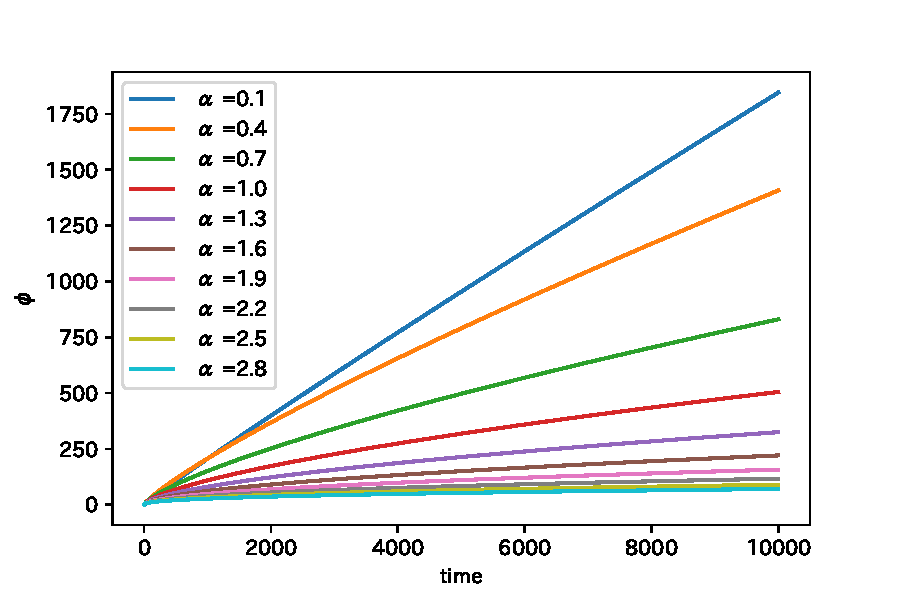
\includegraphics{figure/Attracter_cal.pdf}
  \caption{$\alpha$をいろいろ変えて式\eqref{eq:1.12.6}を数値計算。}
  \label{fig:calculation_of_eq:1.12.6}
  \centering
  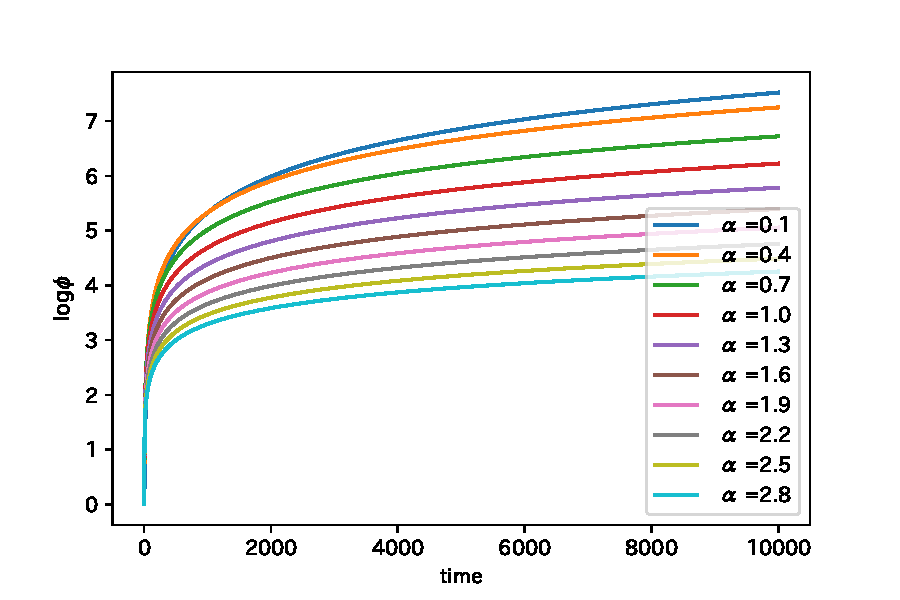
\includegraphics{figure/Attracter_cal_log.pdf}
  \caption{$\alpha$をいろいろ変えて式\eqref{eq:1.12.6}を数値計算の指数部分を見るために$\log$をとったもの。}
  \label{fig:calculation_of_eq:1.12.6_log}
\end{figure}%
これを理解するために、式\eqref{eq:1.12.7}で与えられる解に摂動$\delta \varphi$を与えてみよう($\varphi \to \varphi +\delta \varphi$)。
二階微分、一階微分の部分は線形だからそのままで、$\varphi^{-\alpha -1}\to(\varphi + \delta \varphi)^{-\alpha-1}\approx \varphi^{-\alpha -1} -(1+\alpha)\varphi^{-\alpha-2} \cdot \delta \varphi$
なので、これらより、$\varphi$は以下の式を満たす。
\begin{align}
  0=\delta \ddot{\varphi}+\frac{3}{2 t} \delta \dot{\varphi}+\alpha(1+\alpha) M^{4+\alpha} \varphi^{-\alpha-2} \delta \varphi=\delta \ddot{\varphi}+\frac{3}{2 t} \delta \dot{\varphi}+\frac{(6+\alpha)(1+\alpha)}{(2+\alpha)^{2} t^{2}} \delta \varphi
\end{align}%
そして、これは、$\delta\varphi = t^{\beta}$と解を仮定して代入すれば、
\begin{align}
  \delta \varphi \propto t^{\gamma}, \quad \gamma=-\frac{1}{4} \pm \sqrt{\frac{1}{16}-\frac{(6+\alpha)(1+\alpha)}{(2+\alpha)^{2}}}
\end{align}%
という形の二つの独立な解を得る。
$\alpha>0$なので、ルートの中身は負。少し計算するとわかる。
\begin{align}
  \frac{1}{16}-\frac{(6+\alpha)(1+\alpha)}{(2+\alpha)^{2}} = \frac{-15\alpha^2 - 92 \alpha -92}{16(\alpha+2)^2} < 0
\end{align}%
なので、平方根は$\alpha>0$で虚数を与えるから、$\delta \varphi$の解は、両方とも$t$が増加するとともに、$t^{-1/4}$のように減衰する。
この理由のため、$t\to0$において\footnote{文脈的に、$t$が増加すると、この解に近づくのだから、$t \to \infty$かと思ったがそうではないようだ。}、式\eqref{eq:1.12.7}のように振る舞う式\eqref{eq:1.12.6}の
特解は、トラッカー(tracker)解として知られている。
スカラー場の初期条件に対し、スカラー場が現在までにトラッカー解に近づくべしという条件(そのような初期条件は「アトラクションの内湾(basin of attraction)」と知られている)という物理的な理由は特にないのであるが、この要請によって、スカラー場の現在の進化が初期条件に依存しなくなるため、たった2つの自由パラメータ$M$と$\alpha$を持つクインテッセンスモデルが得られるという実用上の利便性がある。

放射のエネルギー密度が非相対論的物質のエネルギー密度を下回る時期が来ても、特に何も起こらない。
スカラー場のトラッカー解は、$t^{2/(2+\alpha)}$のように成長し、$\dot{\varphi}^2,V(\varphi)$は、$t^{-2\alpha(2+\alpha)}$のように減少し続ける。
しかし、$\rho_{M}$、$\rho_{R}$はそれぞれ$t^{-2}$、$t^{-8/3}$のようにより早く減少し続けるので、結果として、$\rho_{M}$と$\rho_{R}$が$\rho_{\varphi}$を下回るようになる($\rho_{R}<\rho_{M}\ll \rho_{\varphi}$)。
$\rho_{\varphi}=\rho_{M}$となる時刻での$\varphi$の値が、不明な定数$M$に依存しないのは興味深い。
これを以下では見ていく。
物質優勢での宇宙膨張の時、式(1.5.31)から、$\rho_M = 1/(6\pi G t^2)$と与えられるが、
式\eqref{eq:1.12.2}\footnote{英語版だと、1.1.2と誤植あり。}に、式\eqref{eq:1.12.5}および式\eqref{eq:1.12.7}を代入すれば、%\eqref{eq:1.5.31}$$
\begin{align}
  \rho_{\varphi} \approx M^{\frac{2(4+\alpha)}{2+\alpha}} t^{\frac{-2\alpha}{2+\alpha}}
\end{align}%
を与えるので、$\rho_{\varphi} = \rho_{M}$となる時刻$t_c$は、
\begin{align}
  t_c = \frac{1}{6\pi}\left(G^{-1} M^{\frac{-2(4+\alpha)}{2+\alpha}}\right)^{\frac{2+\alpha}{4}}\\
  t_c \approx M^{-\frac{4+\alpha}{2}} G^{-\frac{2+\alpha}{4}}
\end{align}%
で与えられ、これを式\eqref{eq:1.12.7}に代入すれば、以下の結果を得る。\footnote{僕の備忘録。計算で、$2+\alpha$の部分がうまく消える}
\begin{align}
  \varphi(t_c) \approx G^{-1/2}
\end{align}%

さて、少し状況を変える。$\rho_M$が$\rho_\varphi$を非常に下回れば($\rho_M\ll \rho_{\varphi}$)、式(1.5.37)の$H=\sqrt{\frac{8\pi G \rho_V}{3}}$より、式\eqref{eq:1.12.4}を考えれば、
\begin{align}
  \ddot{\varphi}+\sqrt{24 \pi G \rho_{\varphi}} \dot{\varphi}-\alpha M^{4+\alpha} \varphi^{-\alpha-1}=0
\end{align}%
$\rho_V \to \rho_\varphi$と置き換えた。$\rho_\varphi$は式\eqref{eq:1.12.2}で与えられる。
そして、この時代のトラッカー解は、複雑な時間依存性を持っている。
しかし、十分に時間が経過し、現在よりももっと後の時刻になれば(?)、再び単純な形をとることを見よう。
$\dot{\varphi}$に比例する減衰項は、$\varphi$の成長を妨げることから、最終的に$\dot{\varphi}$は$V(\varphi)$よりも小さくなり、また、$\ddot{\varphi}$に比例する慣性項は、減衰項やポテンシャル項に比べて、無視できるようになると推測できる(これは、4章と10章でのべるインフレーションの理論で重要な役割を果たす「スローロール(slow roll)」条件とよく似ている(らしい))。$\leftarrow$わからない。。。\dag

\end{document}


\section{Intergalactic absorption}\label{sec1-10:Intergalactic-absorption}
\section{Number counts}\label{sec:Number-counts}
\section{Horizons}\label{sec:Horizons}

\part{THE COSMIC MICROWAVE RADIATION BACKGROUND}
\section{Expectations and discovery of the microwave background}
\section{The equilibrium era}
\section{Recombination and last scattering}
\section{The dipole anisotorpy}
\section{The Sunyaev-Zel'dovich effect}
\section{Primary fluctuations in the microwave background: A first look}

\part{THE EARLY UNIVE
